% Template for the submission to:
%   The Annals of Applied Statistics    [AOAS]
%
%%%%%%%%%%%%%%%%%%%%%%%%%%%%%%%%%%%%%%%%%%%%%%
%% In this template, the places where you   %%
%% need to fill in your information are     %%
%% indicated by '???'.                      %%
%%                                          %%
%% Please do not use \input{...} to include %%
%% other tex files. Submit your LaTeX       %%
%% manuscript as one .tex document.         %%
%%%%%%%%%%%%%%%%%%%%%%%%%%%%%%%%%%%%%%%%%%%%%%

\documentclass[aoas]{imsart}

%% Packages
\RequirePackage{amsthm,amsmath,amsfonts,amssymb,centernot,float,import,makeidx,subfiles}
\RequirePackage{natbib}
%\RequirePackage[colorlinks,citecolor=blue,urlcolor=blue]{hyperref}
\RequirePackage{graphicx}% uncomment this for including figures

\startlocaldefs
%%%%%%%%%%%%%%%%%%%%%%%%%%%%%%%%%%%%%%%%%%%%%%
%%                                          %%
%% Uncomment next line to change            %%
%% the type of equation numbering           %%
%%                                          %%
%%%%%%%%%%%%%%%%%%%%%%%%%%%%%%%%%%%%%%%%%%%%%%
%\numberwithin{equation}{section}
%%%%%%%%%%%%%%%%%%%%%%%%%%%%%%%%%%%%%%%%%%%%%%
%%                                          %%
%% For Axiom, Claim, Corollary, Hypothezis, %%
%% Lemma, Theorem, Proposition              %%
%% use \theoremstyle{plain}                 %%
%%                                          %%
%%%%%%%%%%%%%%%%%%%%%%%%%%%%%%%%%%%%%%%%%%%%%%
%%%%%%%%%%%%%%%%%%%%%%%%%%%%%%%%%%%%%%%%%%%%%%
\theoremstyle{plain}
\newtheorem{axiom}{Axiom}
\newtheorem{claim}[axiom]{Claim}
\newtheorem{theorem}{Theorem}[section]
\newtheorem{lemma}[theorem]{Lemma}
\newtheorem{proposition}{Proposition}
\newcommand{\matr}[1]{\mathbf{#1}} % undergraduate algebra version

%%%%%%%%%%%%%%%%%%%%%%%%%%%%%%%%%%%%%%%%%%%%%%
%%                                          %%
%% For Assumption, Definition, Example,     %%
%% Notation, Property, Remark, Fact         %%
%% use \theoremstyle{remark}                %%
%%                                          %%
%%%%%%%%%%%%%%%%%%%%%%%%%%%%%%%%%%%%%%%%%%%%%%
\theoremstyle{remark}
\newtheorem{remark}{remark}
%%%%%%%%%%%%%%%%%%%%%%%%%%%%%%%%%%%%%%%%%%%%
%\theoremstyle{plain}
%\newtheorem{???}{???}
%\newtheorem*{???}{???}
%\newtheorem{???}{???}[???]
%\newtheorem{???}[???]{???}
%%%%%%%%%%%%%%%%%%%%%%%%%%%%%%%%%%%%%%%%%%%%%%
%%                                          %%
%% For Assumption, Definition, Example,     %%
%% Notation, Property, Remark, Fact         %%
%% use \theoremstyle{remark}                %%
%%                                          %%
%%%%%%%%%%%%%%%%%%%%%%%%%%%%%%%%%%%%%%%%%%%%%%
%\theoremstyle{remark}
%\newtheorem{???}{???}
%\newtheorem*{???}{???}
%\newtheorem{???}{???}[???]
%\newtheorem{???}[???]{???}
%%%%%%%%%%%%%%%%%%%%%%%%%%%%%%%%%%%%%%%%%%%%%%
%% Please put your definitions here:        %%
%%%%%%%%%%%%%%%%%%%%%%%%%%%%%%%%%%%%%%%%%%%%%%

\endlocaldefs

\begin{document}

\begin{frontmatter}
%%%%%%%%%%%%%%%%%%%%%%%%%%%%%%%%%%%%%%%%%%%%%%
%%                                          %%
%% Enter the title of your article here     %%
%%                                          %%
%%%%%%%%%%%%%%%%%%%%%%%%%%%%%%%%%%%%%%%%%%%%%%
\title{The Effect of Medicaid Expansion on Non-Elderly Adult Uninsurance Rates Among States that did not Expand Medicaid}
%\title{A sample article title with some additional note\thanksref{T1}}
\runtitle{}
%\thankstext{T1}{A sample of additional note to the title.}

\begin{aug}
%%%%%%%%%%%%%%%%%%%%%%%%%%%%%%%%%%%%%%%%%%%%%%
%%Only one address is permitted per author. %%
%%Only division, organization and e-mail is %%
%%included in the address.                  %%
%%Additional information can be included in %%
%%the Acknowledgments section if necessary. %%
%%%%%%%%%%%%%%%%%%%%%%%%%%%%%%%%%%%%%%%%%%%%%%
\author[A]{\fnms{Max} \snm{Rubinstein}\ead[label=e1]{Heinz College and Department of Statistics and Data Science}} and
\author[A]{\fnms{Amelia} \snm{Haviland}\ead{Heinz College and Department of Statistics and Data Science}}
%%%%%%%%%%%%%%%%%%%%%%%%%%%%%%%%%%%%%%%%%%%%%%
%% Addresses                                %%
%%%%%%%%%%%%%%%%%%%%%%%%%%%%%%%%%%%%%%%%%%%%%%
\address[A]{Carnegie Mellon University, \printead{e1}}

\end{aug}

\begin{abstract}
We estimate the effect of Medicaid expansion on the adult uninsurance rate in states that did not expand Medicaid in 2014 using a novel extension of the synthetic controls approach (\cite{abadie2010synthetic}). The existing literature primarily estimates treatment effects on states that expanded Medicaid. We hypothesize these effects differ: prior to the 2014 expansion, evidence suggested that Medicaid take-up rates are lower among conservative states (\cite{sommers2012understanding}), and Republicans were more likely to govern non-expansion states. We therefore hypothesize that the treatment effect on states that did not expand Medicaid would have been closer to zero than for states that did expand Medicaid. Using data from the American Community Survey (ACS), we estimate the effect on non-expansion states by re-weighting expansion regions to approximately balance the covariates from non-expansion regions. We contribute to the literature on balancing weights by accounting for hierarchical data and measurement error in the covariates when calculating the weights. We estimate that Medicaid expansion would have changed the uninsurance rate by -2.17 percentage points (-3.41, -0.94). These results are smaller in absolute magnitude than existing estimates of the treatment effect on the treated (see, e.g., \cite{courtemanche2017early}). We also provide suggestive (though statistically insignificant) evidence that factors associated with Republican governance may drive this difference.
\end{abstract}

\begin{keyword}
\kwd{Synthetic controls}
\kwd{Balancing weights}
\kwd{Medicaid expansion}
\end{keyword}

\end{frontmatter}
%%%%%%%%%%%%%%%%%%%%%%%%%%%%%%%%%%%%%%%%%%%%%%
%% Please use \tableofcontents for articles %%
%% with 50 pages and more                   %%
%%%%%%%%%%%%%%%%%%%%%%%%%%%%%%%%%%%%%%%%%%%%%%
%\tableofcontents

%%%%%%%%%%%%%%%%%%%%%%%%%%%%%%%%%%%%%%%%%%%%%%
%%%% Main text entry area:

\section{Introduction}

The 2010 Affordable Care Act (ACA) required states to expand their Medicaid eligibility requirements by 2014 to offer coverage to all adults with incomes at or below 138 percent of the federal poverty level (FPL). The United States Supreme Court ruled this requirement unconstitutional in 2012, allowing states to decide whether to expand Medicaid coverage. In 2014, twenty-six states and the District of Columbia expanded their Medicaid programs. From 2015 through 2020 an additional twelve states elected to expand their Medicaid programs. This first wave of expansions in 2014 enabled researchers to examine the effects of Medicaid expansion by using expansion states as ``treated'' states and non-expansion states as ``control'' states. Our primary goal in this paper is to estimate the effect of 2014 Medicaid expansion on non-elderly adult uninsurance rates among states that did not expand Medicaid.

We predict that the treatment effect on non-expansion effect will be smaller in absolute magnitude than in states that expanded Medicaid in 2014. Medicaid take-up rates are lower than 100 percent and historically have varied across states. This variation is partly a function of state discretion in administering programs: for example, program outreach, citizenship verification policies, and application processes differ across states (\cite{courtemanche2017early}). Here we consider how political composition may have driven differences in take-up rates between states. Prior to the 2014 Medicaid expansion, \cite{sommers2012understanding} found that conservative political ideology was associated with lower Medicaid enrollment rates, even after controlling for a variety of other policies. Most importantly, political ideology appears to have largely driven a state's decision to expand Medicaid in 2014. Figure~\ref{fig:stateideology} plots a measure of each state's 2013 institutional ideology score (\cite{berry1998measuring}) by their Medicaid expansion status. Higher values of this score correspond to more liberal government institutions. The red dashed line indicates the mean expansion state score and the gray dashed line indicates the mean non-expansion state score. Figure~\ref{fig:stateideology} illustrates that non-expansion states are more conservative than expansion states. If the differential take-up rates observed by \cite{sommers2012understanding} continue to hold post-expansion, we should expect treatment effects on non-expansion states to be smaller in absolute magnitude than treatment effects on expansion states. 

\begin{figure}[H]
    \begin{center}
    \caption{Government ideology and Medicaid expansion}
    \label{fig:stateideology}
    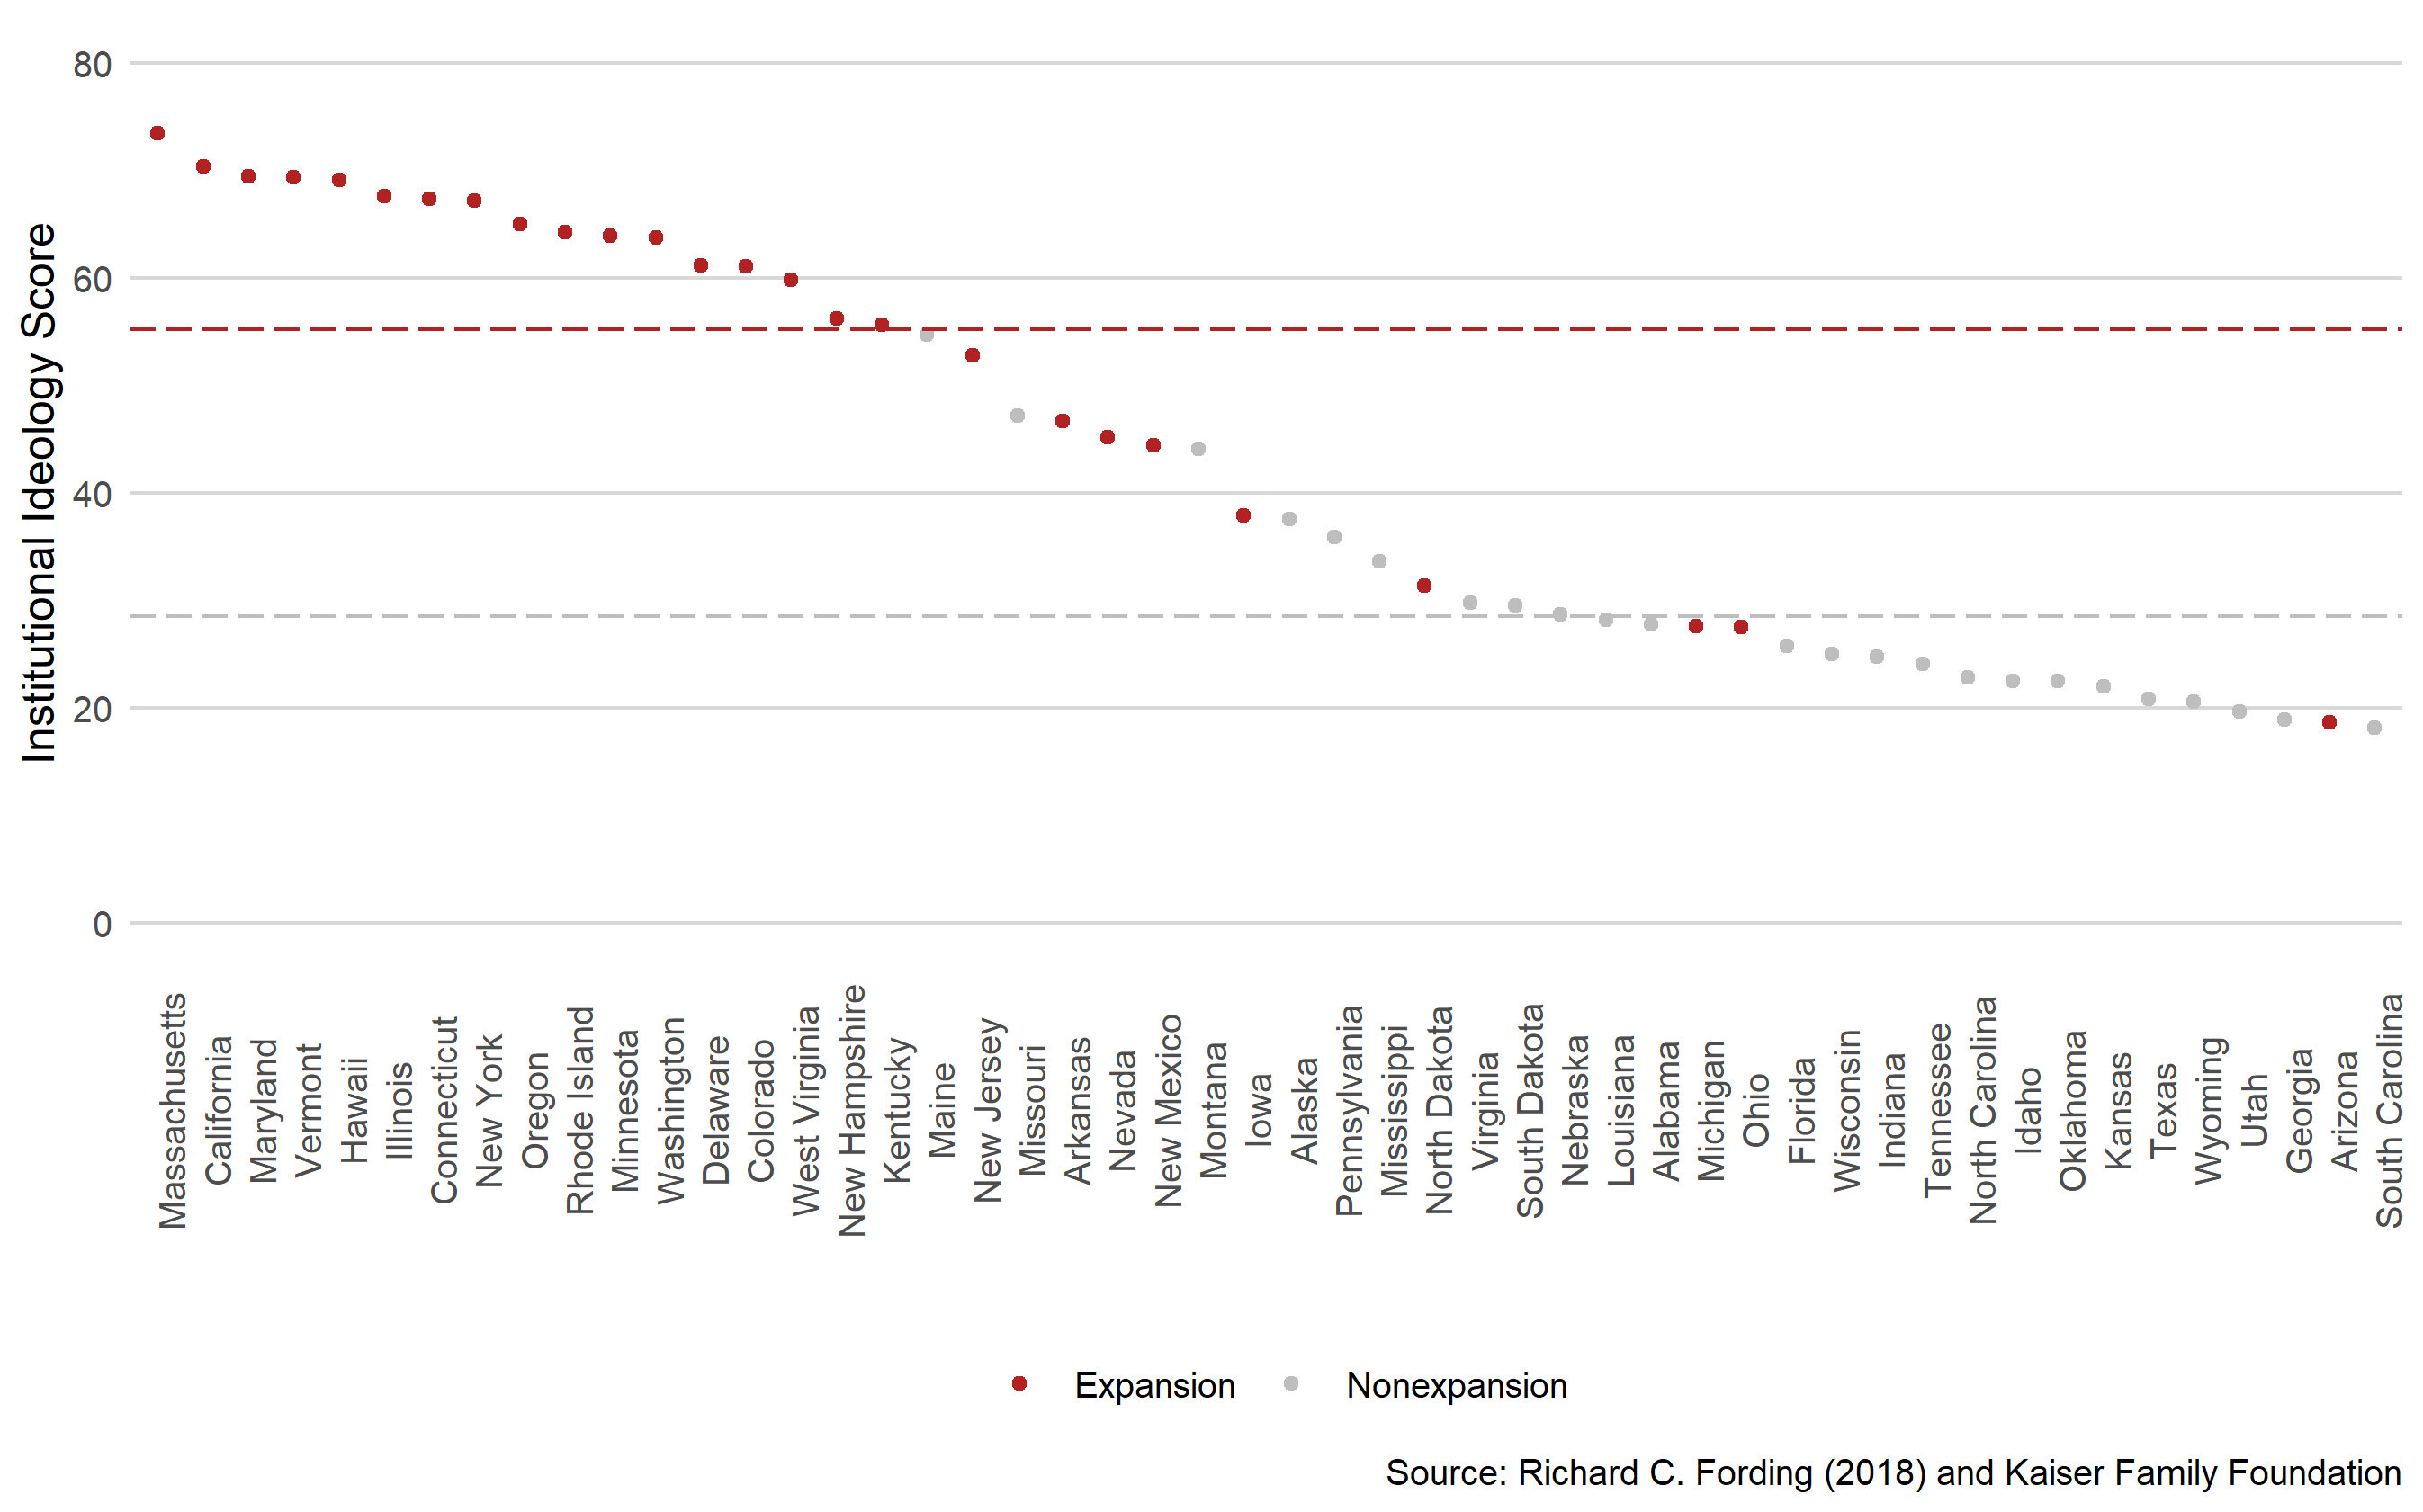
\includegraphics[scale=0.5]{01_Plots/political-expansion-plot.png}
    \end{center}
\end{figure}

This paper makes two methodological contributions to the literature on balancing weights. First, we extend the ``synthetic controls'' framework to estimate the treatment effect on the controls (ETC) using longitudinal data and we clarify the required assumptions. In brief, while balancing on pre-treatment outcomes alone arguably suffices for some synthetic control applications (see, e.g., \cite{botosaru2017role}), because our goal in this setting is to estimate treatment response, we must therefore balance on all covariates that predict treatment response, not just the outcome level absent treatment. Moreover, we cannot simply leverage pre-treatment data to conduct variable selection in this setting. We instead use an implementation of Stable Balancing Weights (\cite{zubizarreta2015stable}) to estimate a set of positive weights to weight the expansion regions to approximately match the covariate distribution of the non-expansion regions. 

Our second contribution is to modify the Stable Balancing Weights (SBW) objective function to account for our data, which is both hierarchical and has several covariates measured with error. Specifically, we use data from the American Community Survey (ACS) aggregated to the consistent public use microdata area (CPUMA) level. These regions nest within states, and using these smaller regions allows us to get better covariate balance. However, as a result, our data both has a hierarchical structure (regions within states) and, because our region-level covariates are estimated from underlying survey data, the sampling variability from our covariate estimates is a form of measurement error which may bias our treatment effect estimates. We first propose a modification of the SBW criterion to account for the hierarchical nature of the data, which disperses the weights more evenly across states. We then leverage the replicate survey weights provided in the ACS microdata to estimate the covariance matrix associated with the sampling variability and use this information to correct for this bias, following the regression calibration literature (see, e.g., \cite{gleser1992importance}). This is the first study we are aware of that attempts to adjust for hierarchical data structure and measurement error in the covariates when using balancing weights. 

The remainder of this paper has the following structure. Section 2 provides an overview of the data and defines the study period, covariates, outcome, and treatment. Section 3 discusses our methods, beginning by defining our target estimand, and then outlining our identification, estimation, and inferential procedures. Section 4 presents our results and sensitivity analyses. Section 5 contains a discussion of the policy relevance of our findings, and Section 6 contains a brief summary. The Appendices contain additional materials, including proofs, summary statistics, and additional results.

\section{Data}

In this section we overview of our data source, the covariates, the outcome, and the treatment assignment.

\subsection{Data Source}

Our primary data source is the annual household and person public use microdata files from the American Community Survey (ACS) from 2011 through 2014. The ACS is an annual survey of approximately three million individuals across the United States. The public use microdata files include information on individuals in geographic areas greater than 65,000 people. The smallest geographic unit contained in these data are public-use microdata areas (PUMAs), arbitrary boundaries that nest within states but not within counties or other more commonly used geographic units. One limitation of these data is a 2012 change in the PUMA boundaries, which do not overlap well with the previous boundaries. As a result, the smallest possible geographic areas that nest both PUMA coding systems are known as consistent PUMAs (CPUMAs). The United States contains 1,075 total CPUMAs, with states ranging from having one CPUMA (South Dakota, Montana, and Idaho) to 123 CPUMAs (New York). Our primary dataset (discussed in Section~\ref{sssec:txassign} contained 929 CPUMAs among 46 states. The average total number of sampled individuals per CPUMA across the four years is 1,001; the minimum number of people sampled was 334 and the maximum is 23,990. Importantly, this survey is a repeated cross-section rather than a longitudinal dataset of individuals over time.

\subsection{Study period}

We begin our analysis in 2011 following \cite{courtemanche2017early}, who note that several other aspects of the ACA were implemented in 2010 -- including the provision allowing for dependent coverage until age 26, and the elimination of co-payments for preventative care -- and likely induced differential shocks across states. We also restrict our post-treatment period to 2014: several additional states expanded Medicaid in 2015, including Indiana, Michigan, and Pennsylvania. However, these states did not expand Medicaid contemporaneously with the 2014 ACA provisions. Without additional assumptions, this second-year expansion cannot help us estimate the effect of the 2014 expansion. 

\subsection{Covariates}

We use the underlying individual-level ACS survey data and accompanying survey weights to aggregate the data at the CPUMA level. We choose our covariates to approximately align with those considered in \cite{courtemanche2017early} and that are likely to be potential confounders. Because we are ultimately interested in calculating rates, these variables include both the numerator and denominator counts.\footnote{When viewing the denominator variables as random, these ratio estimators will in general be biased. This bias, however, decreases quickly with the sample size (is $O(n^{-1})$). Given that our CPUMA sample sizes are all over 300, we treat these estimates as unbiased in our analysis.}

Using the ACS survey weights, we first estimate: the total non-elderly adult population for each year 2011-2014; the total labor force population (among non-elderly adults) for each year 2011-2013; and the total number of households averaged from 2011-2013. We also construct an average of the total non-elderly adult population from 2011-2013. These are our denominator variables. For our numerator counts, we estimate the total number of: females; whites; people of Hispanic ethnicity; people born outside of the United States; citizens; people with disabilities; married individuals; people with less than a high school education, high school degrees, some college, or college graduates or higher; people living under 138 percent of the FPL, between 139 and 299 percent, 300 and 499 percent, more than 500 percent, and who did not respond to the income survey question; people aged 19-29, 30-39, 40-49, 50-64; households with one, two, or three or more children, and households that did not respond about the number of children.\footnote{Number of children and income to poverty ratio were the only two variables with missing data in the underlying microdata.} We average these estimated counts using the ACS survey weights from 2011-2013. For each individual year from 2011-2013, we estimate the total number of people who were unemployed and uninsured at the time of the survey (calculated among all non-elderly adults and all non-elderly adults within the labor force, respectively). We divide the numerator counts by the corresponding denominator counts to estimate the percentage in each category. For the demographics, these include the average number of non-elderly adults from 2011-2013. For the time-varying variables, we use the corresponding year (where uninsurance rates are calculated as a fraction of the labor force rather than the non-elderly adult population). We also calculate the average non-elderly adult population growth and the average number of households to adults across 2011-2013. 

In addition to the ACS microdata, we use 2010 Census data to calculate the approximate percentage of people living within an ``urban'' area for each CPUMA. Finally, we include three state-level covariates reflecting the partisan composition of each state's government in 2013. Specifically, we use data from the National Conference of State Legislatures (NCLS) to generate an indicator for states with a Republican governor, an indicator for states with Republican control over the lower legislative chamber, and an indicator for states with Republican control over both chambers of the legislature and the governorship.\footnote{Nebraska is the only state with a unicameral legislature; moreover, the legislature is technically non-partisan. We nevertheless classified them as having Republican control of the legislature.} 

\subsection{Outcome}

Our outcome of interest is the non-elderly adult uninsurance rate in 2014, which we denote using $Y$. While take-up among the Medicaid-eligible population is a more natural outcome, we choose the non-elderly adult uninsurance rate for two reasons, one theoretic and one practical. First, Medicaid eligibility in the post-period is likely endogenous: Medicaid expansion may affect an individual's income and poverty levels, which in general define Medicaid eligibility. A second reason is to align our study with others to compare our results with the existing literature, and this is the outcome that \cite{courtemanche2017early} use. One drawback of using this outcome is that the simultaneous adoption of other ACA provisions in 2014 more clearly affects this rate in a way that a more targeted group might not be.

\subsection{Treatment assignment} \label{sssec:txassign}

While some states expanded Medicaid and other states did not, assigning a binary treatment status simplifies a more complex reality. There are three reasons to be cautious about this simplification. First, states differed substantially in their Medicaid coverage policies prior to 2014: with perfect data we might consider Medicaid expansion as a continuous treatment with values proportional to the number of newly eligible individuals. The challenge though is correctly identifying newly eligible individuals in the data (see \cite{frean2017premium}, who attempt to address this). Second, \cite{frean2017premium} note that five states (California, Connecticut, Minnesota, New Jersey, and Washington) and the District of Columbia adopted partial limited Medicaid expansions prior to 2014. \footnote{\cite{kaestner2017effects} and \cite{courtemanche2017early} also consider Arizona, Colorado, Hawaii, Illinois, Iowa, Maryland, and Oregon to have had early expansions.} Lastly, timing is an issue: among the states that expanded Medicaid in 2014, Michigan's expansion did not go into effect until April 2014, while New Hampshire's expansion did not occur until September 2014.

Our primary analysis excludes New York, Vermont, Massachusetts, Delaware, and the District of Columbia from our pool of expansion regions, because these regions had comparable Medicaid coverage policies prior to 2014 (\cite{kaestner2017effects}). We also exclude New Hampshire because it did not expand Medicaid until September 2014. While Michigan expanded Medicaid in April 2014, we leave this state in our pool of treated states. We consider the remaining expansion states as ``treated'' and the non-expansion states as ``control'' states. We later consider the sensitivity of our results to these classifications by removing the early expansion states noted by \cite{frean2017premium}. Our final dataset contains aggregated statistics for all of the above variables for 925 CPUMAs in our non-expansion and our pool of expansion states. There are 414 CPUMAs among 24 non-expansion states and 515 CPUMAs among 22 expansion states. When we exclude the early expansion states for sensitivity analyses, we are left with 296 CPUMAs across 17 states.

\section{Methods}
\label{sec:methods}

In this section we present our causal estimand, identifying assumptions, estimation strategy, and inferential procedure.

\subsection{Estimand}

Our goal is to estimate the average effect 2014 Medicaid expansion would have had on the non-elderly adult uninsurance rate in states that did not expand Medicaid. Let $c$ index a CPUMA, $s$ index the state, and $t$ index the time period. Let $n_1$ be the number of treated CPUMAs, $n_0$ be the number of control CPUMAs, and $n$ be the total number of CPUMAs. Similarly, let and $m = m_1 + m_0$ states (with $m_1$ and $m_0$ defined analogously). Each state has $p_s$ CPUMAs. Since we are only interested in the counterfactual at time $T = 2014$, we simplify notation by removing this variable and the subscript and write our formal estimand as:

\begin{equation}
\psi = \psi^1 - \psi^0 &= n_0^{-1}\sum_{s, c: A_s = 0} Y_{sc}^{A_s = 1} - Y_{sc}^{A_s = 0}
\end{equation}

The challenge is predicting the counterfactual uninsurance rates in 2014 for states that did not expand Medicaid expansion had they expanded their Medicaid eligibility requirements. We therefore require causal assumptions to tie this counterfactual quantity to our observed data.\footnote{The 2014 Medicaid expansion occurred simultaneously with the implementation of several other major ACA provisions, including (but not limited to) the creation of the ACA-marketplace exchanges, the individual mandate, health insurance subsidies, and community-rating and guaranteed issue of insurance plans (\cite{courtemanche2017early}). Almost all states broadly implemented these reforms beginning January 2014. Conceptually we think of the other ACA components as a state-level treatment ($R$) separate from Medicaid expansion ($A$). Therefore, our total estimated effect may also include interactions between these policy changes; however, we do not attempt to separately identify these effects. Because the ACA implementation and Medicaid expansion may vary over time, we do not try to generalize these results beyond 2014.} 

\subsection{Identification}

The following causal assumptions are necessary (though not sufficient) to enable us to identify our target parameter from the data: consistency, no unmeasured confounding, no anticipatory treatment effects, and positivity of treatment assignment. We explain these assumptions in detail and their consequences below. We additionally invoke several parametric assumptions to help us identify our causal parameter given the measurement error in our covariates.

Consistency implies that a CPUMA's potential outcome under some treatment assignment is equal to the observed factual outcome given that same treatment assignment: 

\begin{align*}
Y_{sc}^{A_{sc} = a} = Y_{sc} \mid A_{sc} = a
\end{align*}

In other words, we assume that one region's treatment assignment does not affect another region's observed outcome. This is a standard assumption, but is often not realistic. Violations of this assumption are likely in our setting: for example, \cite{frean2017premium} find evidence that Medicaid expansion drove previously eligible but uninsured individuals to enroll in Medicaid in both expansion and non-expansion states. Signing the potential bias from this violation requires redefining the causal estimand: for example, we might consider the treatment effect on the untreated given that all states have expanded Medicaid, where the contrast is against where only the observed expansion states expanded Medicaid. If spillovers occurred in equal proportions across each region, and the magnitude of the spillovers increase with the total number of treated regions, then the true effect would be larger in absolute magnitude than the estimated estimated using the observed data. We could consider other estimands or assumptions to get different predictions about the sign of the bias; however, this is beyond the scope of this paper.

We next assume that there were no anticipatory treatment effects. Letting treatment occur at time $T$, we have that for $t < T$:

\begin{align*}
Y_{sct} = Y_{sct}^0
\end{align*}

This assumption is necessary because we are conditioning on pre-treatment outcomes. If these outcomes were affected by the treatment before it were implemented, these covariates would be endogenous. Anticipatory treatment effects may occur if plans to expand Medicaid induce uninsured but Medicaid-eligible individuals to enroll in Medicaid prior to expansion. We do not think these violations occurred in large enough numbers to substantially affect our results. Instead, we address a more concerning version of this violation: the fact that several states allowed certain counties to expand Medicaid prior to 2014. We therefore test the sensitivity of our results to the exclusion of these states.

Third, we assume no unmeasured confounding; that is, that at time $T$ the potential outcomes for each CPUMA are independent of the state-level treatment assignment conditional on the population-level CPUMA and state-level covariates $X_{sc}$, a $q$ dimensional vector of covariates (which includes pre-treatment outcomes):

\begin{align*}
Y_{sc}^a \perp A_{sc} \mid X_{sc}
\end{align*}

While unverifiable, we believe it is reasonable here given our rich covariate set. To be explicit, we believe that the potential uninsurance rates for each CPUMA are independent of the treatment assignment conditional on the percentage of uninsured individuals in each year of the pre-treatment period, the percentage of unemployed individuals in each year of the pre-treatment period, the average population growth, the average ratio of households to non-elderly adult population, the state's political composition, the average proportion of households with one, two, or three or more children during the pre-treatment period, the average proportion of households who did not respond about their number children, and the average proportion of individuals during the pre-treatment period with given demographics noted above (age group, sex, white, Hispanic ethnicity, U.S. citizenship, foreign born, income-to-poverty group (including non-response), disability status, urban residence, and educational attainment group). 

Finally, we assume positivity of treatment assignment; that is, that all states had some non-zero probability of being treated 

\begin{align*}
\pi(X_{1s}, ..., X_{p_ss}) > \epsilon
\end{align*}

where the propensity score is some function of the covariate values for each CPUMA and where $\epsilon > 0$. Positivity violations can cause a lack of covariate overlap in the observed data. Overlap is an issue in this study. We address this in multiple ways that we outline in our estimation strategy below. 

These assumptions are sufficient to non-parametrically identify our causal estimand if we observed the true outcomes and covariates. Unfortunately, because our covariates are estimated using the ACS data. We model our observed data as consisting of mean-unbiased estimates of the true covariate values, i.e. $J_{sc} = Y_{sc} + \xi_{sc}$ and $W_{sc} = X_{sc} + v_{sc}$. Importantly, $Y_{sc}^a \perp A_{sc} \mid X_{sc} \centernot\implies J_{sc}^a \perp A_{sc} \mid W_{sc}$. The use of these proxies may therefore bias our estimates. We rely on several modeling assumptions to correct for this bias.

We begin by placing restrictions on the errors in the outcome measurement $\xi_{sc}$. First, we assume that these errors are uncorrelated with the true values of $Y_{sc}$. Second, we assume that $\xi_{sc}$ is uncorrelated with $X_{sc}$. Third, we assume that $\xi_{sc}$ are uncorrelated with the errors in the covariate measurements ($v_{sc}$). This first and second assumptions are reasonable given that the measurement error in this context is simply sampling variability. We believe the third assumption is also reasonable given that our outcomes are measured on a different cross-section than our covariates. 

We next assume that the true potential outcomes are linear in the true covariates $X_{sc}$. Specifically, we assume that the following model generates the potential non-elderly adult uninsurance rate under treatment $A = a$:

\begin{equation}
Y_{sc}^a = \alpha_a + X_{sc}^T\beta_a + \epsilon_{sc} + c_s
\end{equation}

We assume that the errors $\epsilon_{sc}$ and $c_s$ are independent from each other and across time (i.e., we rule out serial-correlation), that these errors are invariant to the intervention, and are uncorrelated with the true covariates. This model then allows us to identify $\psi^a$ in terms of our model parameters (see Appendix A); specifically, we have that $\psi^a = \alpha_a + \bar{X}_0^T\beta_a$, where $\bar{X}_0$ is the vector of mean covariate values among the control units. Moreover, we can substitute $J_{sc}$ for $Y_{sc}$ in this equation, and add $\xi_{sc}$ to the error term without affecting this identification.\footnote{We also assume that $\xi_{sc}$ is uncorrelated with the errors in the outcome model, so that the total variance of these stochastic terms is simply the sum of the individual variance terms.} 

We still have the problem that we observe $W_{sc}$ instead of $X_{sc}$. We again assume that these errors are uncorrelated with the true covariate values (i.e. are sampling variability). Let $\mu_a = \mathbb{E}\{X_{sc} \mid W_{sc}, A = a\}$. By linearity, we know that

\begin{equation}
    J_{sc} = \eta_a(W_{sc})^T\beta + (X_{sc} - \eta_a(W_{sc}))^T\beta + \xi_{sc} + \epsilon_{sc} + v_s 
\end{equation}

If we knew $\eta_a$, we could estimate this model using the observed data $(\matr{J}, \matr{W})$. The approach we follow here is known as ``regression calibration'' in the measurement-error literature. In particular, we assume the following model for $\eta_a$:

\begin{align*}
\eta_a(W_{sc}) = \mu_a + \kappa^T(W_{sc} - \mu_a)
\end{align*}

where $\kappa = (\Sigma_{XX} + \Sigma_{vv})^{-1}\Sigma_{XX}$. This assumptions motivating this model is that $W_{sc} = X_{sc} + v_{sc}$, where $(X_{sc}, v_{sc}) \stackrel{iid}\sim MVN((\mu_a, 0)^T, \Sigma)$ and $\Sigma$ is block-diagonal consisting of elements $\Sigma_{XX}$ and $\Sigma_{vv}$. Given sufficient auxillary data to estimate $\kappa$, we can use these models to consistently estimate of $\psi$. We discuss this further below and in Appendix A (see also \cite{gleser1992importance}).

\subsection{Estimation}

We first outline our procedure to estimate the ETC given our assumptions above, using a novel extension of Stable Balancing Weights. Using this estimation method, we then outline our strategy to examine whether there might be treatment effect heterogeneity with respect to Republican governance.

\subsection{Estimating the ETC}

We outline our estimation strategy first emphasizing how our method differs from the synthetic controls approach, which motivates our use of the SBW objective. Second, we explain a modification we make to the SBW criterion to address the hierarchical data structure (which we call H-SBW) that reduces the variance of our estimator under our assumption of within-state correlation of our model errors. Third, we connect our estimator to the regression calibration literature by generating weights that balance a linear prediction of the true covariates $\hat{\eta}_a(W_{sc})$ using the observed covariates $W_{sc}$. 

We also test the sensitivity of our estimator to a ridge-augmented version, following the suggestion of \cite{ben2018augmented}; this allows us to achieve better covariate balance by extrapolating beyond the support of the data. As a separate sensitivity check, we estimate a different causal parameter -- the overlap average treatment effect (OATE) -- as discussed in \cite{li2018balancing}. Estimating this effect does not require extrapolation, but rather changing the target estimand. We discuss this further below.

Similar to synthetic controls applications, we seek to generate a set of positive weights that balance the means of covariates for the treated units to the mean of covariates for the control units. Assume that we observe the true covariate matrices $\matr{X}_1 = (X_{1,1}^T, ..., X_{1, q}^T)$ and $\matr{X}_0$ (defined similarly), and the true outcomes $Y$, and let $\bar{\matr{X}}_0$ be the mean covariate values in the non-expansion region. Ideally, there exists some $\gamma^\star$ such that for $\delta = 0$: 

\begin{align*}
\lvert \matr{X}_{1, r}^T\gamma^\star - \bar{\matr{X}}_{0, r} \lvert \le \delta_r \ \ \ (r = 1, ..., q) \\
\gamma_{sc}^\star > 0, 1^T\gamma^\star = 1
\end{align*}

We could then estimate $\psi$ as

\begin{equation}\label{eqn:psi}
\hat{\psi} = \sum_{s: A_s = 1}^{m_1}\sum_{c = 1}^{p_s}\gamma_{sc}^\star Y_{sc} - n_0^{-1}\sum_{s: A_s = 0}^{m_0}\sum_{c = 1}^{p_s}Y_{sc}
\end{equation}

The assumption that the outcomes (absent treatment) follow a linear factor model frequently motivates the synthetic controls approach; here we instead assume no unobserved confounding and assume that the outcomes given treatment are a linear function of the covariates: $\mu_1(X_{sc}) = \alpha_1 + X_{sc}^T\beta_1$. The bias of our estimator (again assuming we observed $X_{sc}$), is therefore less than or equal to $\lvert\beta\rvert^T\delta = 0$ (see, e.g., \cite{zubizarreta2015stable}). The challenge, however, is that for any given dataset we have no guarantee that any such $\gamma^\star$ exists that exactly balances the covariates; we therefore need some method of determining how to prioritize which parts of the covariate distribution we wish to balance to minimize this bias.

This is where estimating the ETC contrasts with the commonly used synthetic control approach used to estimate the ETT: \cite{abadie2010synthetic} determine how to prioritize covariate balance by training their model on pre-treatment outcomes (\cite{kaul2015synthetic} shows that often the most relevant covariates simply become the pre-treatment outcomes). Because in that setting the counterfactual value $Y^0_{sct}$ is actually observed for $t \le T_0$, \cite{abadie2010synthetic} are able to leverage this data to select the covariates that best predict these values. By contrast we never observe $Y^1_{sct}$ (or a mean-unbiased proxy for it) prior to treatment. Without additional assumptions, we cannot use the pre-treatment data to learn which covariates matter most for determining this potential outcome.

Moreover, the problem of predicting treatment response also makes estimating the ETC more challenging to estimate than the ETT. In particular, we likely care more about balancing ``auxillary covariates'' (covariates that are not pre-treatment outcomes) in our setting than the traditional synthetic controls setting. To see this, assume that $\mu_0$ is linear in the covariates, including the pre-treatment outcomes. We might reasonably believe the coefficients on the auxillary covariates are close to zero once we condition on pre-treatment outcomes. As a result, the bias induced by remaining imbalances on the auxillary covariates would be small. On the other hand, assuming $\mu_1$ is also linear in the same covariates, the coefficients on this model could be much larger, even after conditioning on pre-treatment outcomes, because these coefficients are highly predictive of treatment response. If our weights fail to balance these covariates, we expect that our estimates of $\mu_0$ will in general have less bias than our estimates of $\mu_1$. In summary, estimating the ETC requires a greater understanding of how the covariates are related to treatment response than the ETT; moreover, we cannot learn this information by using pre-treatment outcomes.

We therefore estimate the ETC by using a variation of SBW that we call H-SBW.\footnote{Specifically, we use a modified implementation of Noah Griefer's ``optweight'' package in R, available on github.com/mrubinst757} This procedure allows us to estimate the minimum variance weights that satisfy user-specified balance constraints. Let $\hat{\eta}_1(W_1)$ be a matrix of estimates of $\eta_1(W_1)$ and $\bar{W}_0$ be a vector of estimates of the covariates for the non-expansion region.\footnote{Because $\bar{W}_0$ and $\bar{X}_0$ are equal in expectation, the use of this target will not contribute to any asymptotic bias of our estimator.} We generate weights that solve the following program:

\begin{align*}
&\min_{\gamma} \quad \sum_{s: A_s = 1}^{m_1}(\sum_{c = 1}^{p_s} \gamma_{sc}^2 + \sum_{c \ne d}\rho \gamma_{sc}\gamma_{sd})\\
&\text{ subject to } \lvert \sum_{s,c: A_s = 1}\hat{\eta}_1(W_{sc, r})^T\gamma_{sc} - n_0^{-1}\sum_{s,c: A_s = 0} W_{sc, r} \lvert \le \delta_r  \ \ \ (r = 1, ..., q) \\
&\gamma_{sc} > 0, 1^T\gamma = 1
\end{align*}

We then estimate $\psi$ using Equation~\ref{eqn:psi}, substituting $J_{sc}$ for $Y_{sc}$.

This modification, which we call H-SBW, is a simple modification of the SBW objective, which sets $\rho = 0$ and reweights the imputed observations $\hat{\eta_1(W_{sc})}$ rather than the observed $W_{sc}$. We discuss these differences shortly, but first note that both programs allow the user to specify covariate-level balance constraints using the vector $\delta$. When estimating the ETC, we lean heavily on assumptions to justify our choice of $\delta$; in particular, we use a priori domain knowledge about which covariates are most likely to be important predictors of treatment effect heterogeneity when setting $\delta$. However, we also must choose $\delta$ to something that is feasible given the data. 

For our application, we constrain $\delta$ to be 0.05 percentage points for pre-treatment outcomes, 0.15 percentage points for pre-treatment unemployment rates. We believe these are the most likely factors associated with treatment response, so we prioritize balancing these covariates. For the remaining covariates, we let $\delta$ be 0.5 percentage points for average population growth and household to adult ratio, 1 percentage point for female, Hispanic ethnicity, white race, age category, disability, and number of children category; 2 percentage points for urban, citizenship, education category, income-to-poverty category, student, and foreign-born; and 25 percentage points for the Republican governance indicators. We choose these constraints primarily on feasibility concerns, and for our variance estimates, we reduce these initial constraints when this constraint set becomes infeasible.

We now discuss how H-SBW differs from SBW, beginning with the criterion. The motivation of the SBW criterion, which is equivalent to ours with $\rho = 0$, is to produce the minimum variance weights for a fixed $\delta$. This produces the minimum variance estimator within the constraint set if, for example, the errors in the outcome model are independent and identically distributed. In our setting we allow for possible state-level dependencies, potentially reducing the efficiency of the SBW estimator. To address this situation, we add the tuning parameter $\rho$; this parameter attempts to uniformly disperse the weights across states. This objective produces the minimum variance estimator within the constraint set if we assume a constant (and known) within-state correlation of the errors ($\rho$) and constant variance across units. We discuss this objective in more detail and provide simulation results in Rubinstein et al. (2021) (pre-print not yet available); broadly speaking, we can think of H-SBW being to SBW what generalized least squares (GLS) is to ordinary least squares (OLS): both SBW and OLS can produce unbiased estimates of model parameters; however, H-SBW and GLS can produce efficient estimators assuming a particular block-matrix correlation structure in the outcome errors. 

A more important departure from SBW comes in the constraint set: rather than balancing on the observed covariate values $W_{sc}$, we instead balance on the adjusted estimates $\hat{\eta}_1(W_{sc})$. The estimation error in these CPUMA-level covariates can bias our estimate of $\psi^1$. In Appendix A, we consider the super-population target $\psi^{1, sp} = \mathbb{E}\{Y_{sc}^1 \mid A_{sc} = 0\}$ and show that under the classical errors-in-variables model, the bias for the SBW estimator that balances on the observed covariates $W$ and sets $\delta = 0$ is equivalent to the bias of a linear combination of coefficient estimates from the OLS-based regression estimator. Specifically, for either estimator:

\begin{equation}
\mathbb{E}\{\hat{\psi}^{1} - \psi^{1, sp}\} = (\mu_0 - \mu_1)^T(\kappa - I_d)\beta_1
\end{equation}

The intuition for this result is as follows: exact balancing weights estimate an implicit $\beta$ on a subset of the data where we have sufficient overlap. We can therefore think of SBW as returning a solution to some weighted-least squares problem. If we assume that the outcome model holds across all of the data, WLS and OLS are estimating the same $\beta$; therefore, the bias that effects the least squares solution will have the same effect on the WLS, and therefore SBW, solution. In Appendix A, Proposition 2, we further show that if we had access to $\eta_1$, we can obtain an unbiased estimate by reweighting $\eta_1(W_{sc})$.\footnote{For the finite-sample parameter we're interested in here, the estimator will have some finite-sample bias.} Of course, in practice we do not know $\eta_1$ but must estimate it using auxillary data. In Appendix A, Proposition 3, we show that we can obtain a consistent of $\psi^{1, sp}$ when balancing on an estimate of $\eta_1$ using auxillary data. 

We now discuss how we estimate $\eta_a$. The key is that the ACS data contains replicate survey weights provided at the individual-level which allows us to estimate the variability in each CPUMA's observed covariate values. Specifically, we use these weights to estimate $\hat{\Sigma_{vv, sc}}$, and then use this information along with the observed data to estimate $\hat{\eta}_a$. We consider two versions of this procedure. Our preferred version accounts for the differential measurement error due to the highly variable sample sizes used to calculate each covariate. Specifically, letting $s_{sc}$ be the $q$ dimensional vector of sample sizes for unit $sc$, we consider the model $\sqrt{s}_{sc}v_{sc} \stackrel{iid}\sim MNV(0, \Sigma_{vv})$. This model allows us to generate a separate $\kappa_{sc}$ for each unit using getting the full data for each estimate. As a secondary estimate, we follow the traditionally used approaches which average over all observed variance estimates $\hat{\Sigma}_{vv, sc}$ to estimate a single $\kappa$ for all units. Further details about these procedures are available in Appendix B.

This is the first application we are aware of to use ``regression calibration'' approach in the context of balancing weights to address the problem of measurement error. We emphasize two critical assumptions for using this procedure in our context: (1) the outcome model is linear in the true covariates; and (2) the measurement error in the outcome is uncorrelated with the measurement error in the covariates. The first assumption is strong, though often used in practice. The second assumption is reasonable, because our outcomes are estimated from a different cross-section of individuals than our covariates. 

Finally, because we are unable to reduce the balance constraints to an optimal level, following the recent literature on synthetic controls, we test the sensitivity of our results to these imbalances by using ridge-regression augmented weights \cite{ben2018augmented}. Letting $\matr{\hat{X}}_1$ be the matrix of adjusted covariates, and $\gamma^{hsbw}$ be our H-SBW weights, we standardize our weights to sum to one and estimate the regression-augmented weights:

\begin{equation}
\gamma^{aug} = \gamma^{hsbw} + (\matr{\hat{X}}_1^T\gamma^{hsbw} - \bar{\matr{W}}_0)^T(\matr{\hat{X}}_1^T\Omega^{-1}\matr{\hat{X}}_1 + \lambda I_d)^{-1}\matr{\hat{X}}_1^T\Omega^{-1}
\end{equation}

where $\Omega$ is a block diagonal matrix with diagonal entries equal to one and the within-group off diagonals equal to $\rho$. We choose $\lambda$ so that the remaining imbalances all fall within 0.1 percentage points (see \cite{ben2018augmented} for more details on the connection between these weights and ridge-regression). The cost of this procedure is that we must extrapolate from the support of the data, and therefore rely more heavily on our modeling assumptions. In our results we consider estimators using SBW ($\rho = 0$), H-SBW ($\rho = 0.2$), and ridge-augmented versions of SBW and H-SBW that we call BC-SBW and BC-HSBW. We focus our discussion on our preferred estimator, H-SBW, and its ridge augmented version BC-HSBW. 

\subsection{Effect heterogeneity}

Our secondary research hypothesis is that the ETC is lower in absolute magnitude than the ETT due to treatment effect heterogeneity with respect to Republican governance. We can first investigate this by comparing our point estimate to existing estimates of the ETT. However, we also wish to investigate this question more directly using our data. Partitioning the covariate matrix $\matr{X}$ into groups $(\matr{S}, \matr{V})$, where $\matr{V}$ are the Republican governance indicators and $\matr{S}$ are all other covariates, we would estimate the following contrast:

$$
\Delta^\star = \mathbb{E}\{Y^1 - Y^0 \mid S = \matr{\bar{S}}_0, V = \matr{\bar{V}}_0 + \tau\} - \mathbb{E}\{Y^1 - Y^0 \mid S = \matr{\bar{S}}_0, V = \matr{\bar{V}}_0\}
$$

for some $\tau < 0$ (that is, we compare the ETC against a demographically comparable but less Republican region). Our research hypothesis implies that this contrast is negative. However, this is challenging to estimate in practice because of the difficulty of the lack of covariate overlap, particularly among Republican governance indicators. 

We instead limit our consideration to the association between the Republican governance indicators and the outcome among treated states. In particular, we remove the balance constraints $\delta_v$ associated with covariates $V$ and recalculate an estimate $\hat{\psi}^1_v$ (using weights $\gamma_v$). We then subtract our original point estimate $\hat{\psi}^1_0$ (using weights $\gamma_0$) to generate the difference $\hat{\Delta}^1$. This difference can inform us about the direction of the bias our estimate of $\hat{\psi}^1$ would incur if we removed the balance constraints $\delta_v$. This quantity also approximates the association between covariates $V$ and the outcome on the treated dataset for a data dependent $\tau$:

\begin{align*}
    \hat{\Delta}^1_v &= \sum_{s, c: A_s = 1}(\gamma_v - \gamma_0)J_{sc} \\ 
    &\approx (\matr{X}_1^T(\gamma_v - \gamma_0))^T\beta_1 \\
    &\approx (\matr{V}_1^T(\gamma_v - \gamma_0))^T\beta_{1, v} \\
    &\approx \mathbb{E}\{Y \mid A = 1, S = \matr{\bar{S}}_0, V = \matr{\bar{V}}_0 + \tau\} - \mathbb{E}\{Y \mid A = 1, S = \matr{\bar{S}}_0, V = \matr{\bar{V}}_0\} \\
    &= \mathbb{E}\{Y^1 \mid S = \matr{\bar{S}}_0, V = \matr{\bar{V}}_0 + \tau\} - \mathbb{E}\{Y^1 \mid S = \matr{\bar{S}}_0, V = \matr{\bar{V}}_0\} \\
\end{align*}

where the first equality holds by definition, the first approximation holds from the linearity of the outcome model (and is approximate due to the various error components in the outcome model and the use of adjusted covariates), the second approximation follows because we have only changed the error tolerances on covariates $V$ (and is approximate because some imbalances within $S$ might change within the specified error tolerances $\delta_s$), the third approximation follows from our parametric assumptions (assuming $\delta$ is small), and the final equality by consistency. 

Estimating this contrast can inform by not fully confirm our research hypothesis: in particular, if our hypothesis is incorrect, we should fail to find a positive partial association between Republican governance and the uninsurance rate among the expansion states, i.e. $\hat{\Delta}^1 \ge 0$. On the other hand, if our research hypothesis is correct, it is likely that we will find a positive association, i.e, $\hat{\Delta}^1 < 0$. The key caveat is that the presence of an association does not imply treatment effect heterogeneity unless we make further assumptions on the outcome model absent treatment. However, if the vector of coefficients on covariates $V$ for the outcome model absent treatment $\beta_{0, v} \approx 0$ (or more generally if any linear combination of these coefficients is approximately zero), then $\hat{\Delta}^1_v$ approximates $\Delta^\star_v$. This assumption isn't unreasonable, but could be violated if, for example, more Democratic non-expansion states were more effective at enrolling people in the ACA marketplaces, which were simultaneously implemented along with Medicaid eligibility expansion. 

In addition to the Republican governance indicators, we also examine the influence of four other covariate groups: pre-treatment uninsurance rates and pre-treatment unemployment rates, and three sets of different demographic indicators. Specifically, the first group includes: urban residence, age group, education, citizenship, student, disability, female; the second, white race, Hispanic ethnicity, foreign-born, and income-to-poverty ratio; the third, children category (0, 1, 2, 3+, NA), household to population ratio, and population growth; however, we leave the presentation of these results to Appendix E.

\subsection{Inference}

We use the leave-one-state-out jackknife to estimate the variance $Var(\hat{\psi}^1 \mid W)$ (\cite{cameron2015practitioner}), where we hold our targeted mean fixed at $\bar{\matr{W}}_0$. When our preferred initial choice of $\delta$ does not converge, we programmatically reduce the constraints until the program converges. We calculate this estimator in two ways: first, we condition on our covariate adjustment $\hat{\eta}_1$. This is our preferred estimator. We also calculate $\hat{\eta}_1$ omitting each state in the jackknife procedure. We leave these results to the Appendix.

To estimate $Var(\hat{\psi}^0 \mid W)$ we use an auxillary regression model and use the CR-2 standard error adjustment to estimate the variance of the linear combination $\bar{\matr{W}}_0^T\hat{\beta}_0$ (using the ``clubSandwich'' package in R). Notice that we can run this regression on the original data because $\bar{\matr{W}}_0^T\hat{\beta}_0 = \bar{J}_0$ (which is unbiased for $\psi^0$). In general we expect that the variance of $\hat{\psi}^1$ will dominate the variance of $\hat{\psi}^0$ because in practice the balance constraints will substantially reduce the effective sample size of the treated data. Our total variance estimate is simply the sum of these two variance estimates.

\section{Results}

This section presents the results from our analyses. We begin by presenting statistics on the imbalances in the covariates between the treatment, control, and weighted treatment groups. We then present our primary results, including both our treatment effect estimates and our analysis of the association of Republican governance with the outcome. We conclude by reviewing a series of sensitivity analyses that check the robustness of our results to using excluding the ``early expansion'' states and calculating a different target estimand.

\subsection{Covariate Balance}

Figure~\ref{fig:loveplotc1} shows how our balancing weights reduce the imbalances among covariates with greater than one percentage point difference between the targeted mean in the expansion region and the mean values in the non-expansion region (we target the population-weighted mean of the untreated region).\footnote{The reweighted treatment values use our preferred covariate adjustment $\hat{\eta}_1(W_{sc})$.} Before applying our weights, we see that there are substantial imbalances in the Republican governance indicators, as well as pre-treatment uninsurance and unemployment rates. Our weights drastically reduce these differences; however, some imbalances remain. In particular, imbalances remain in the Republican governance indicators. A complete balance table is available in Appendix D, Table~\ref{tab:baltab1}. Appendix C contains additional summary statistics, including how the original dataset compares to the adjusted dataset. 

\begin{figure}[H]
\begin{center}
    \caption{Balance plot, primary dataset}
    \label{fig:loveplotc1}
    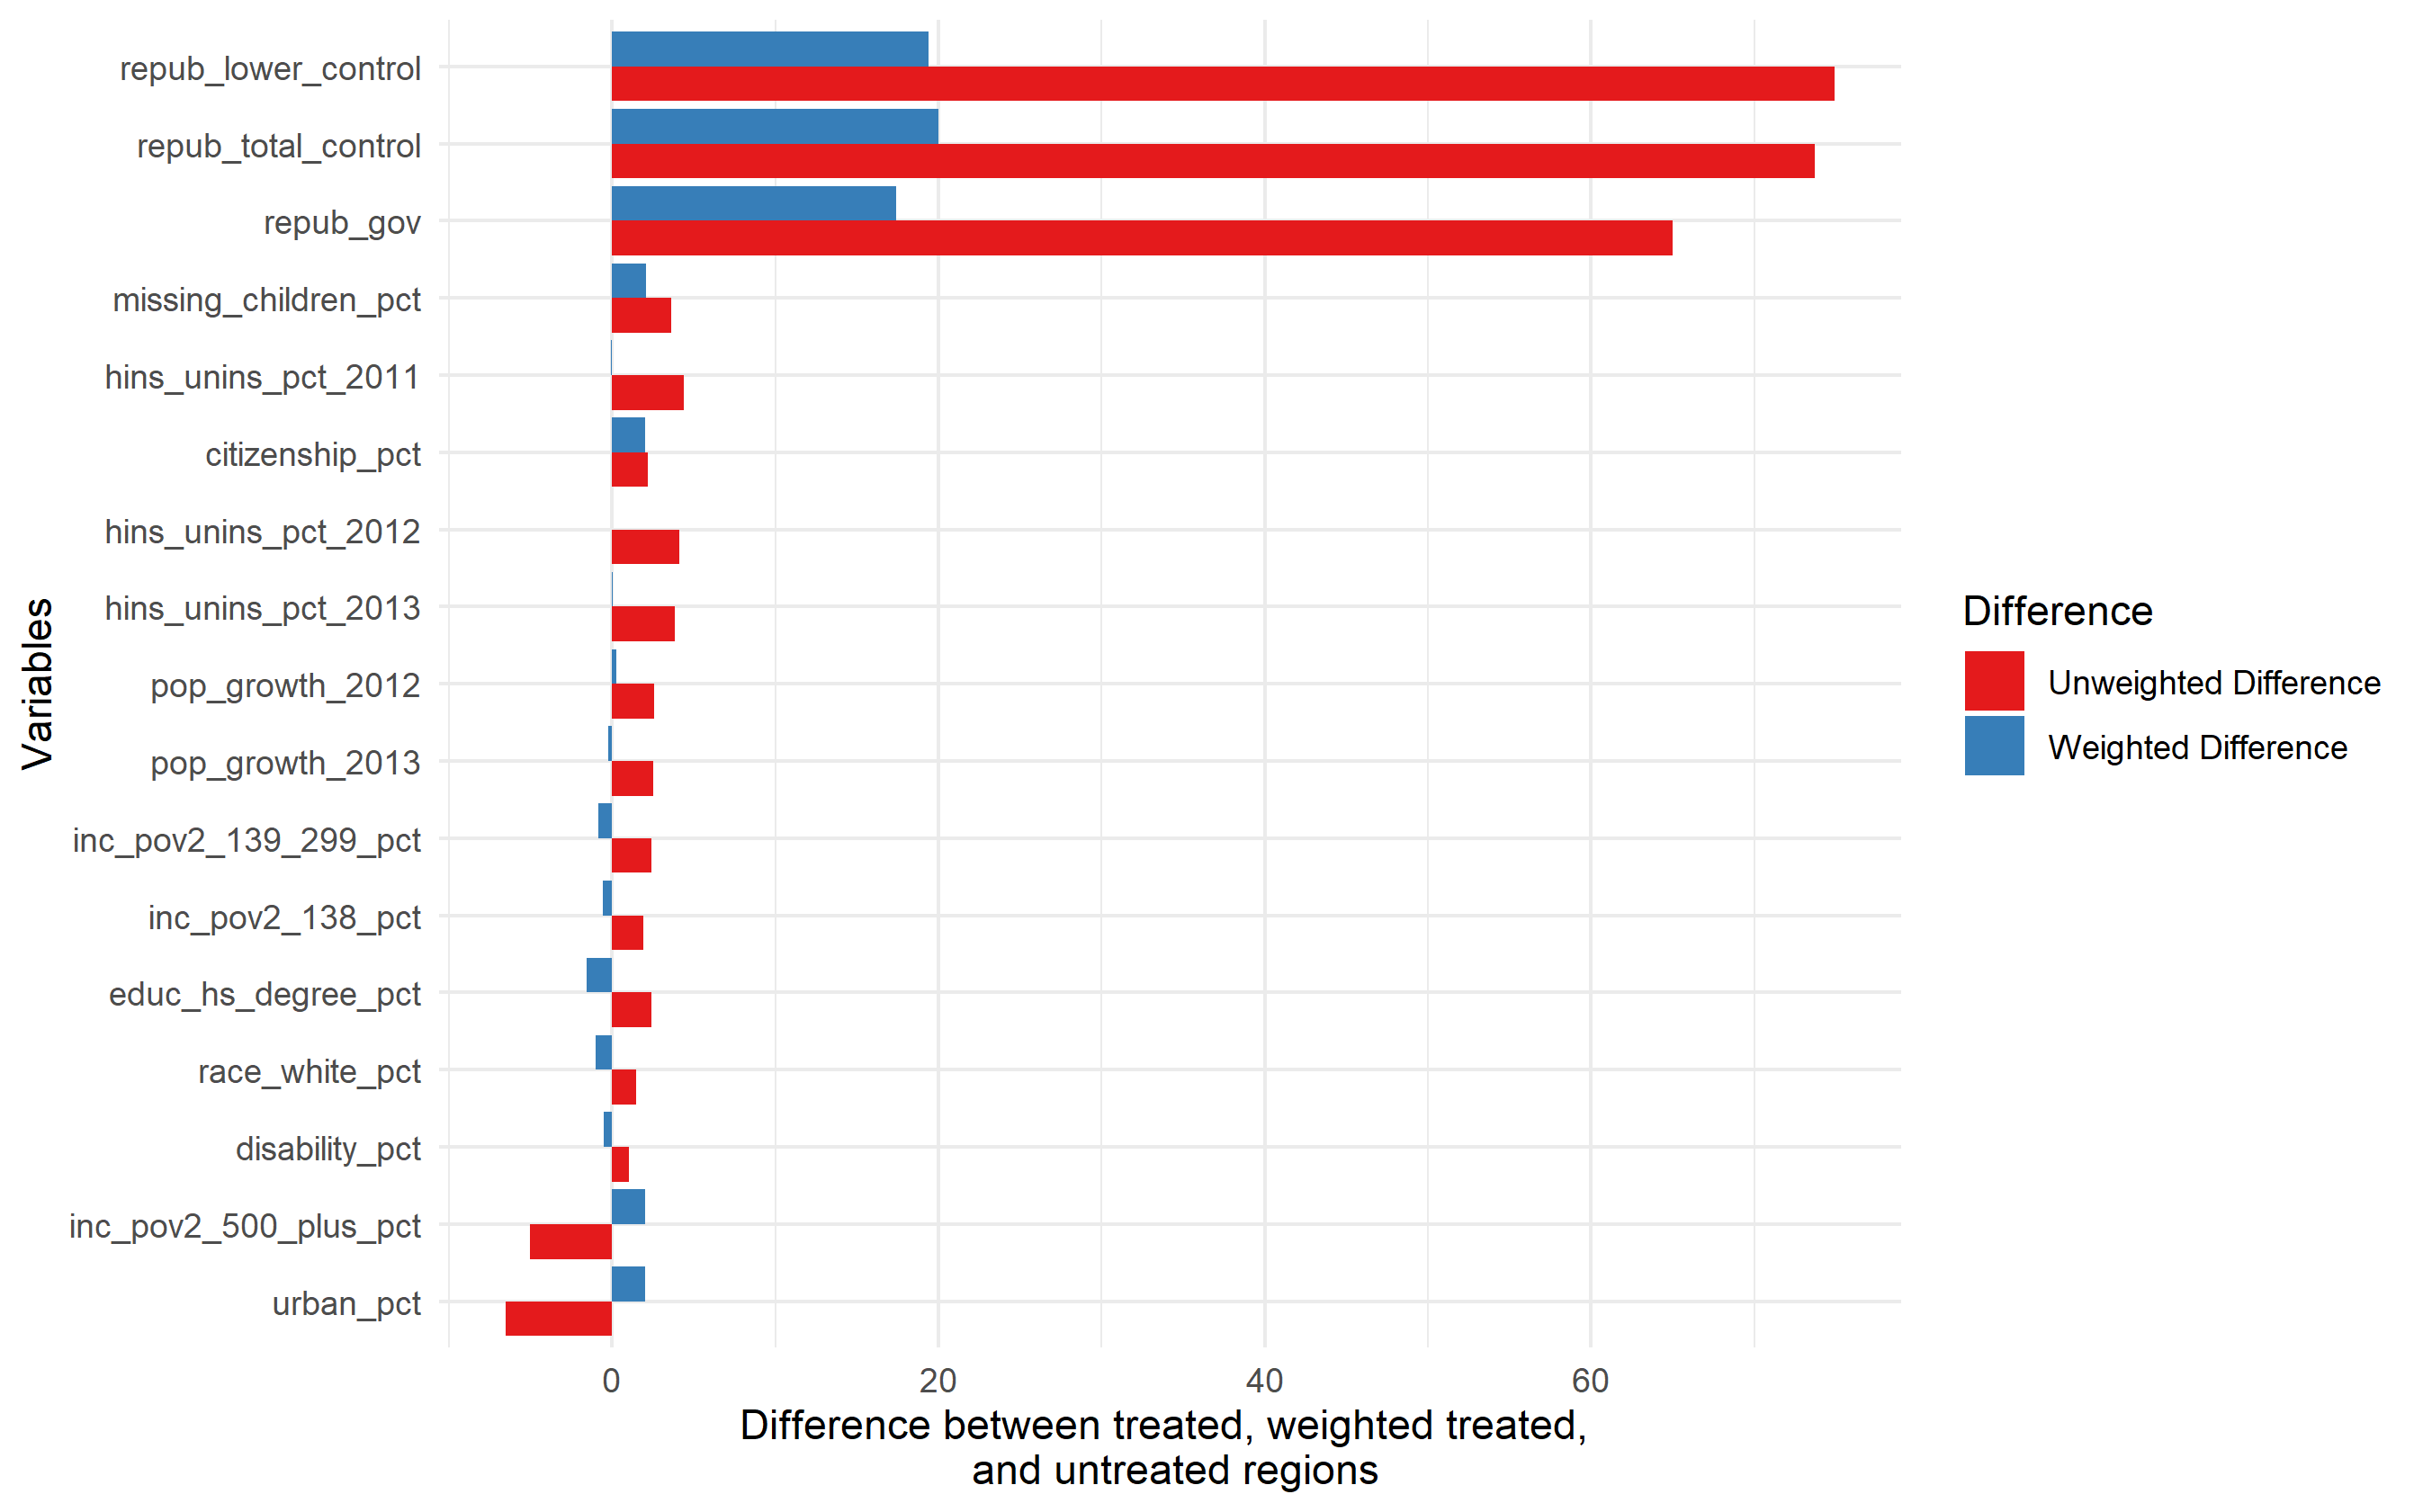
\includegraphics[scale=0.6]{01_Plots/balance-plot-etuc1.png}
\end{center}
\end{figure}

As discussed above, we use ridge-regression augmentation to extrapolate from the data in order to reduce all imbalances within 0.5 percentage points. Figure~\ref{fig:statewghts} shows the total weights summed across states for each estimator: H-SBW and BC-HSBW. This figure sums the negative weights separately from the positive weights to show the extent of the extrapolation. We see that BC-HSBW extrapolates somewhat heavily in order to estimate the counterfactual, particularly for CPUMAs in California. Due to this extensive extrapolation, we therefore prefer the H-SBW estimator, though we compare results against BC-HSBW as a robustness check.\footnote{Note that H-SBW more evenly distributes the weights across states relative to SBW. Appendix D, Figure~\ref{fig:sbwvhsbw} displays this result.}

\begin{figure}[H]
\begin{center}
    \caption{Total weights summed by state, primary dataset}
    \label{fig:statewghts}
    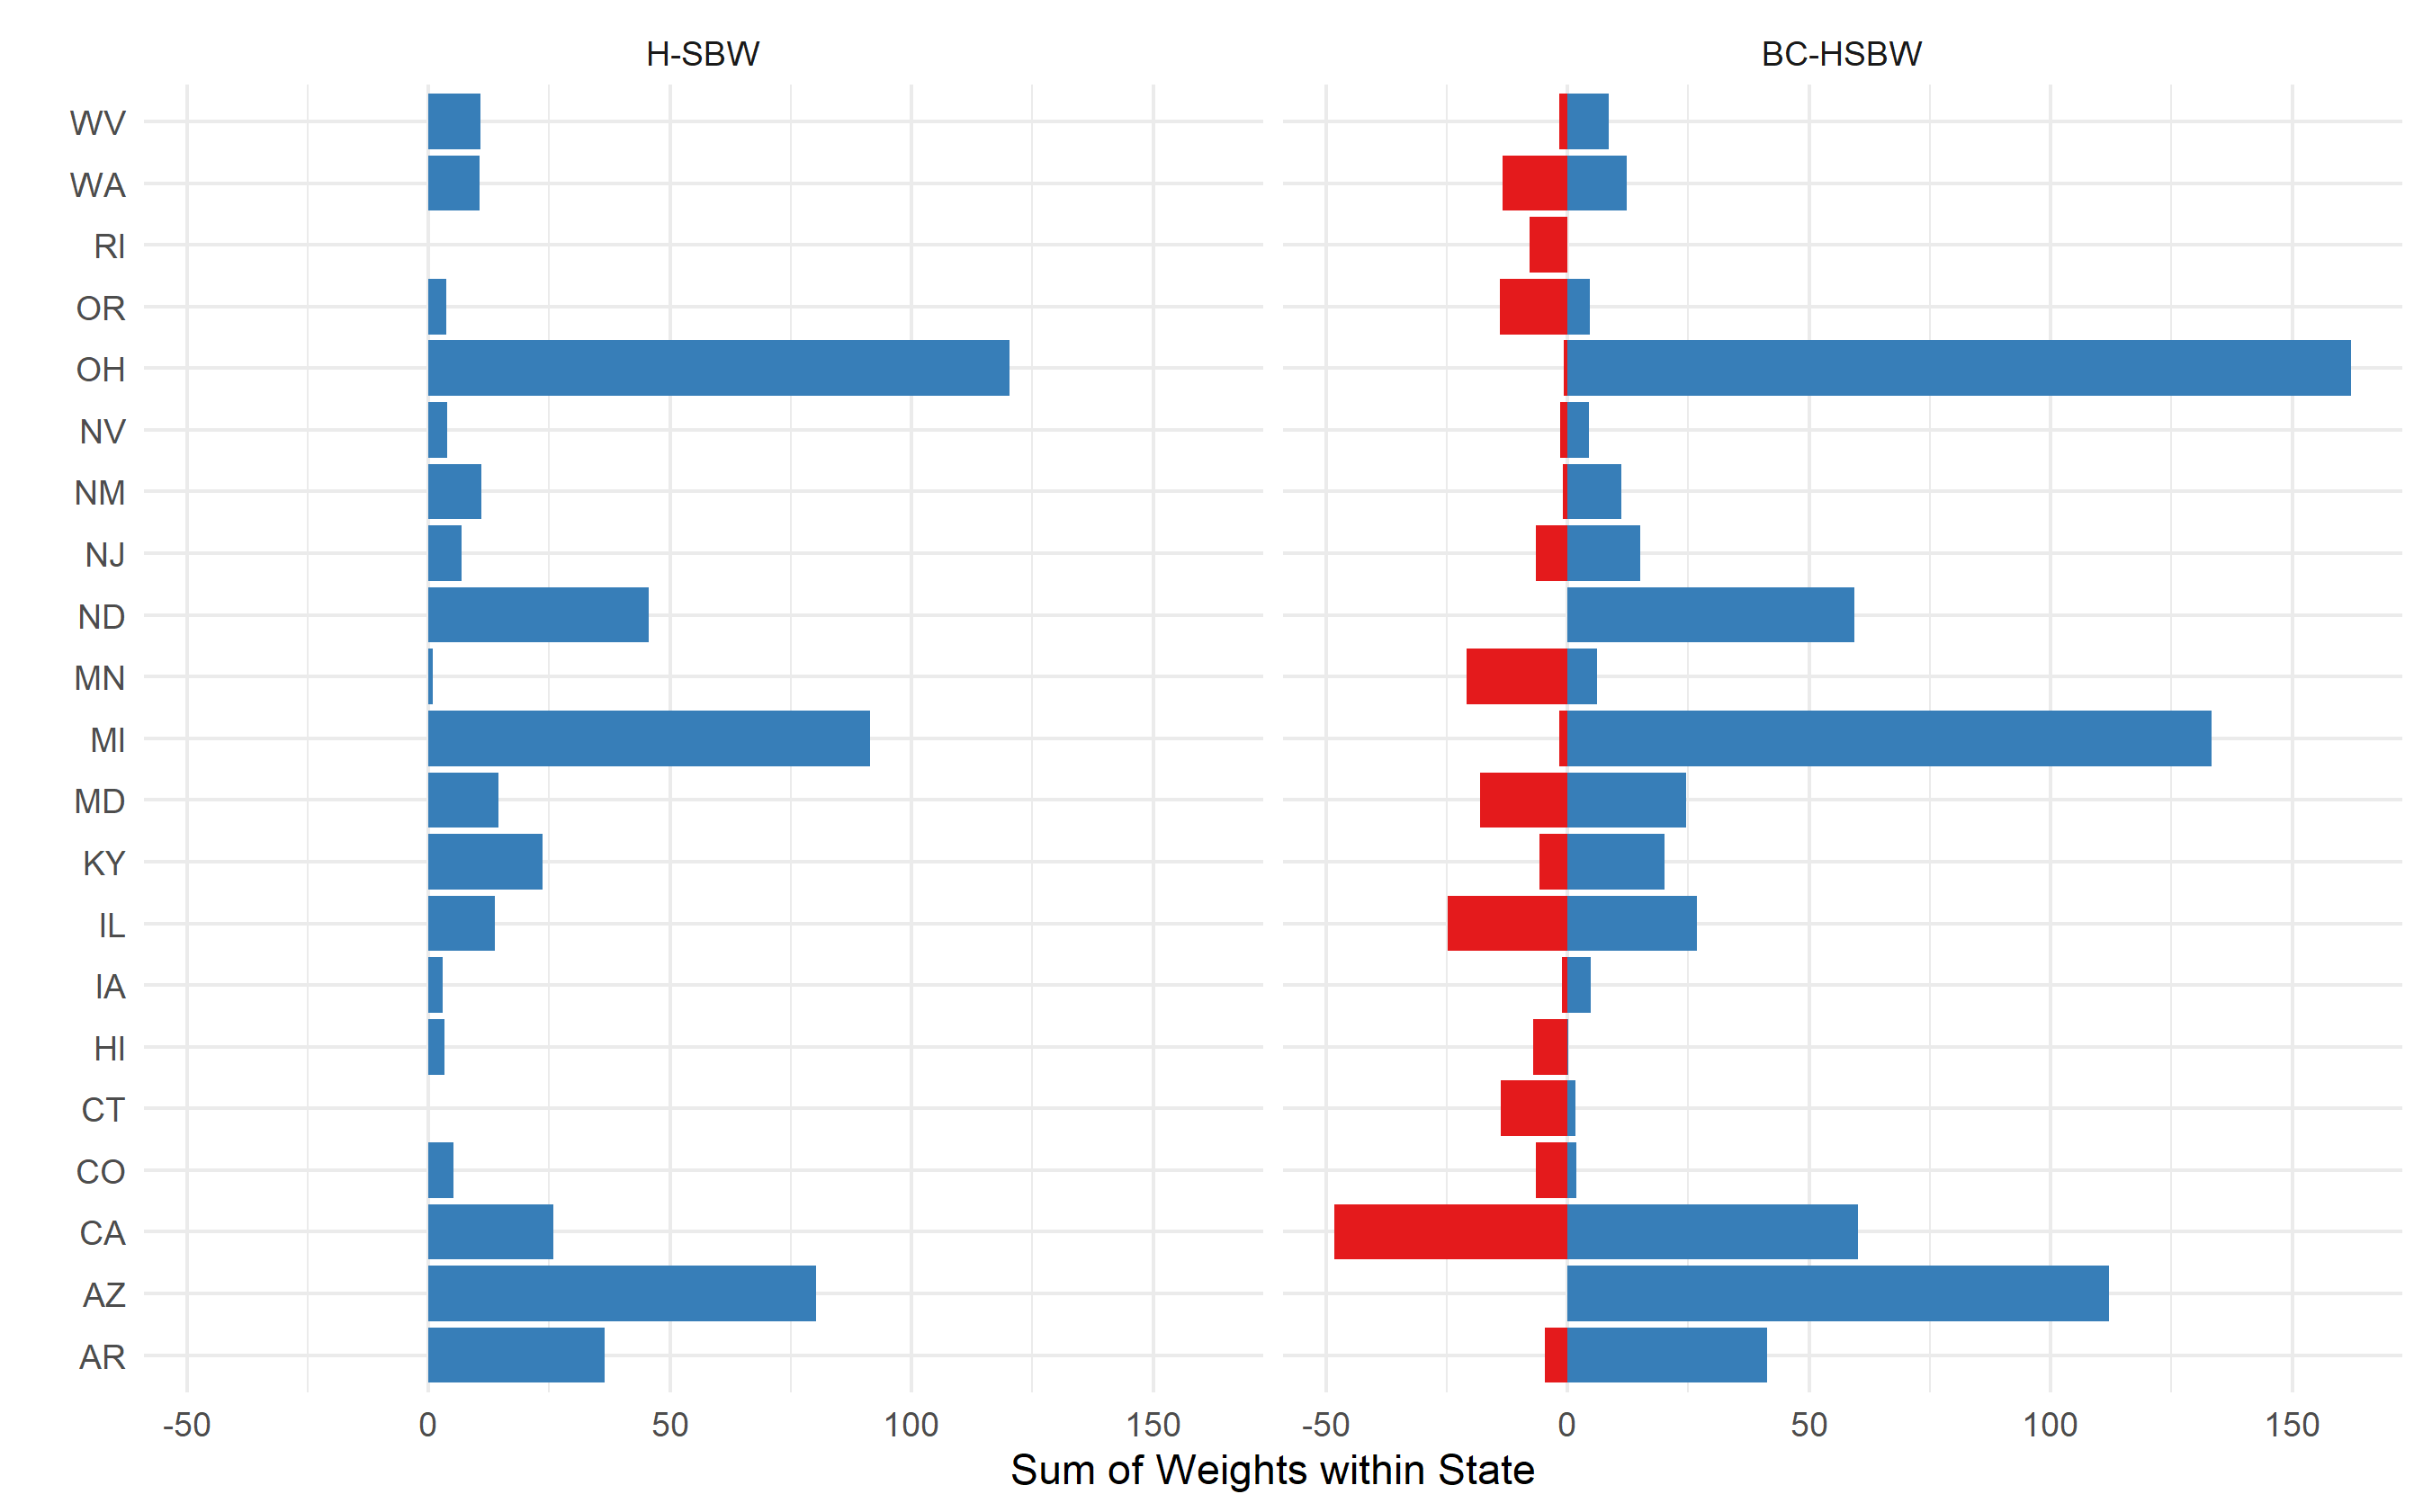
\includegraphics[scale=0.6]{01_Plots/weights-by-state-hsbw-c1.png}
\end{center}
\end{figure}

\subsection{Primary Results}

Using H-SBW we calculate an estimated effect of -2.17 (-3.41, -0.94). In other words, we estimate that had states that did not expand Medicaid in 2014 done so, they would have seen a 2.17 percentage point reduction in their uninsurance rates that year. While remaining imbalances are quite large, the bias-correction makes little substantive difference, yielding an estimate of -2.13 (-3.55, -0.71). These estimates are somewhat larger than the estimates we find running the procedure on our unadjusted covariate estimates: here H-SBW gives an estimated effect of -2.35 (-3.09, -1.61), and the bias corrected estimator yields -2.39 (-3.33, -1.46). This suggests that the measurement error is inducing a non-trivial negative bias, but one that is of a smaller order than the variance. Moreover, we see that using the adjusted covariate set appears to increases the width of the estimated confidence intervals by an even greater amount than the change in the point estimate. This increase is expected because the adjustment procedure generally reduces the variability in the data, thereby requiring that the balancing weights also increase in variability. Figure~\ref{fig:estimators} displays the point estimates from these weighting estimators, as well as estimators using SBW, on the adjusted and unadjusted datasets. Additional results are available in Appendix E.

\begin{figure}[H]
\begin{center}
    \caption{Point estimates}
    \label{fig:estimators}
    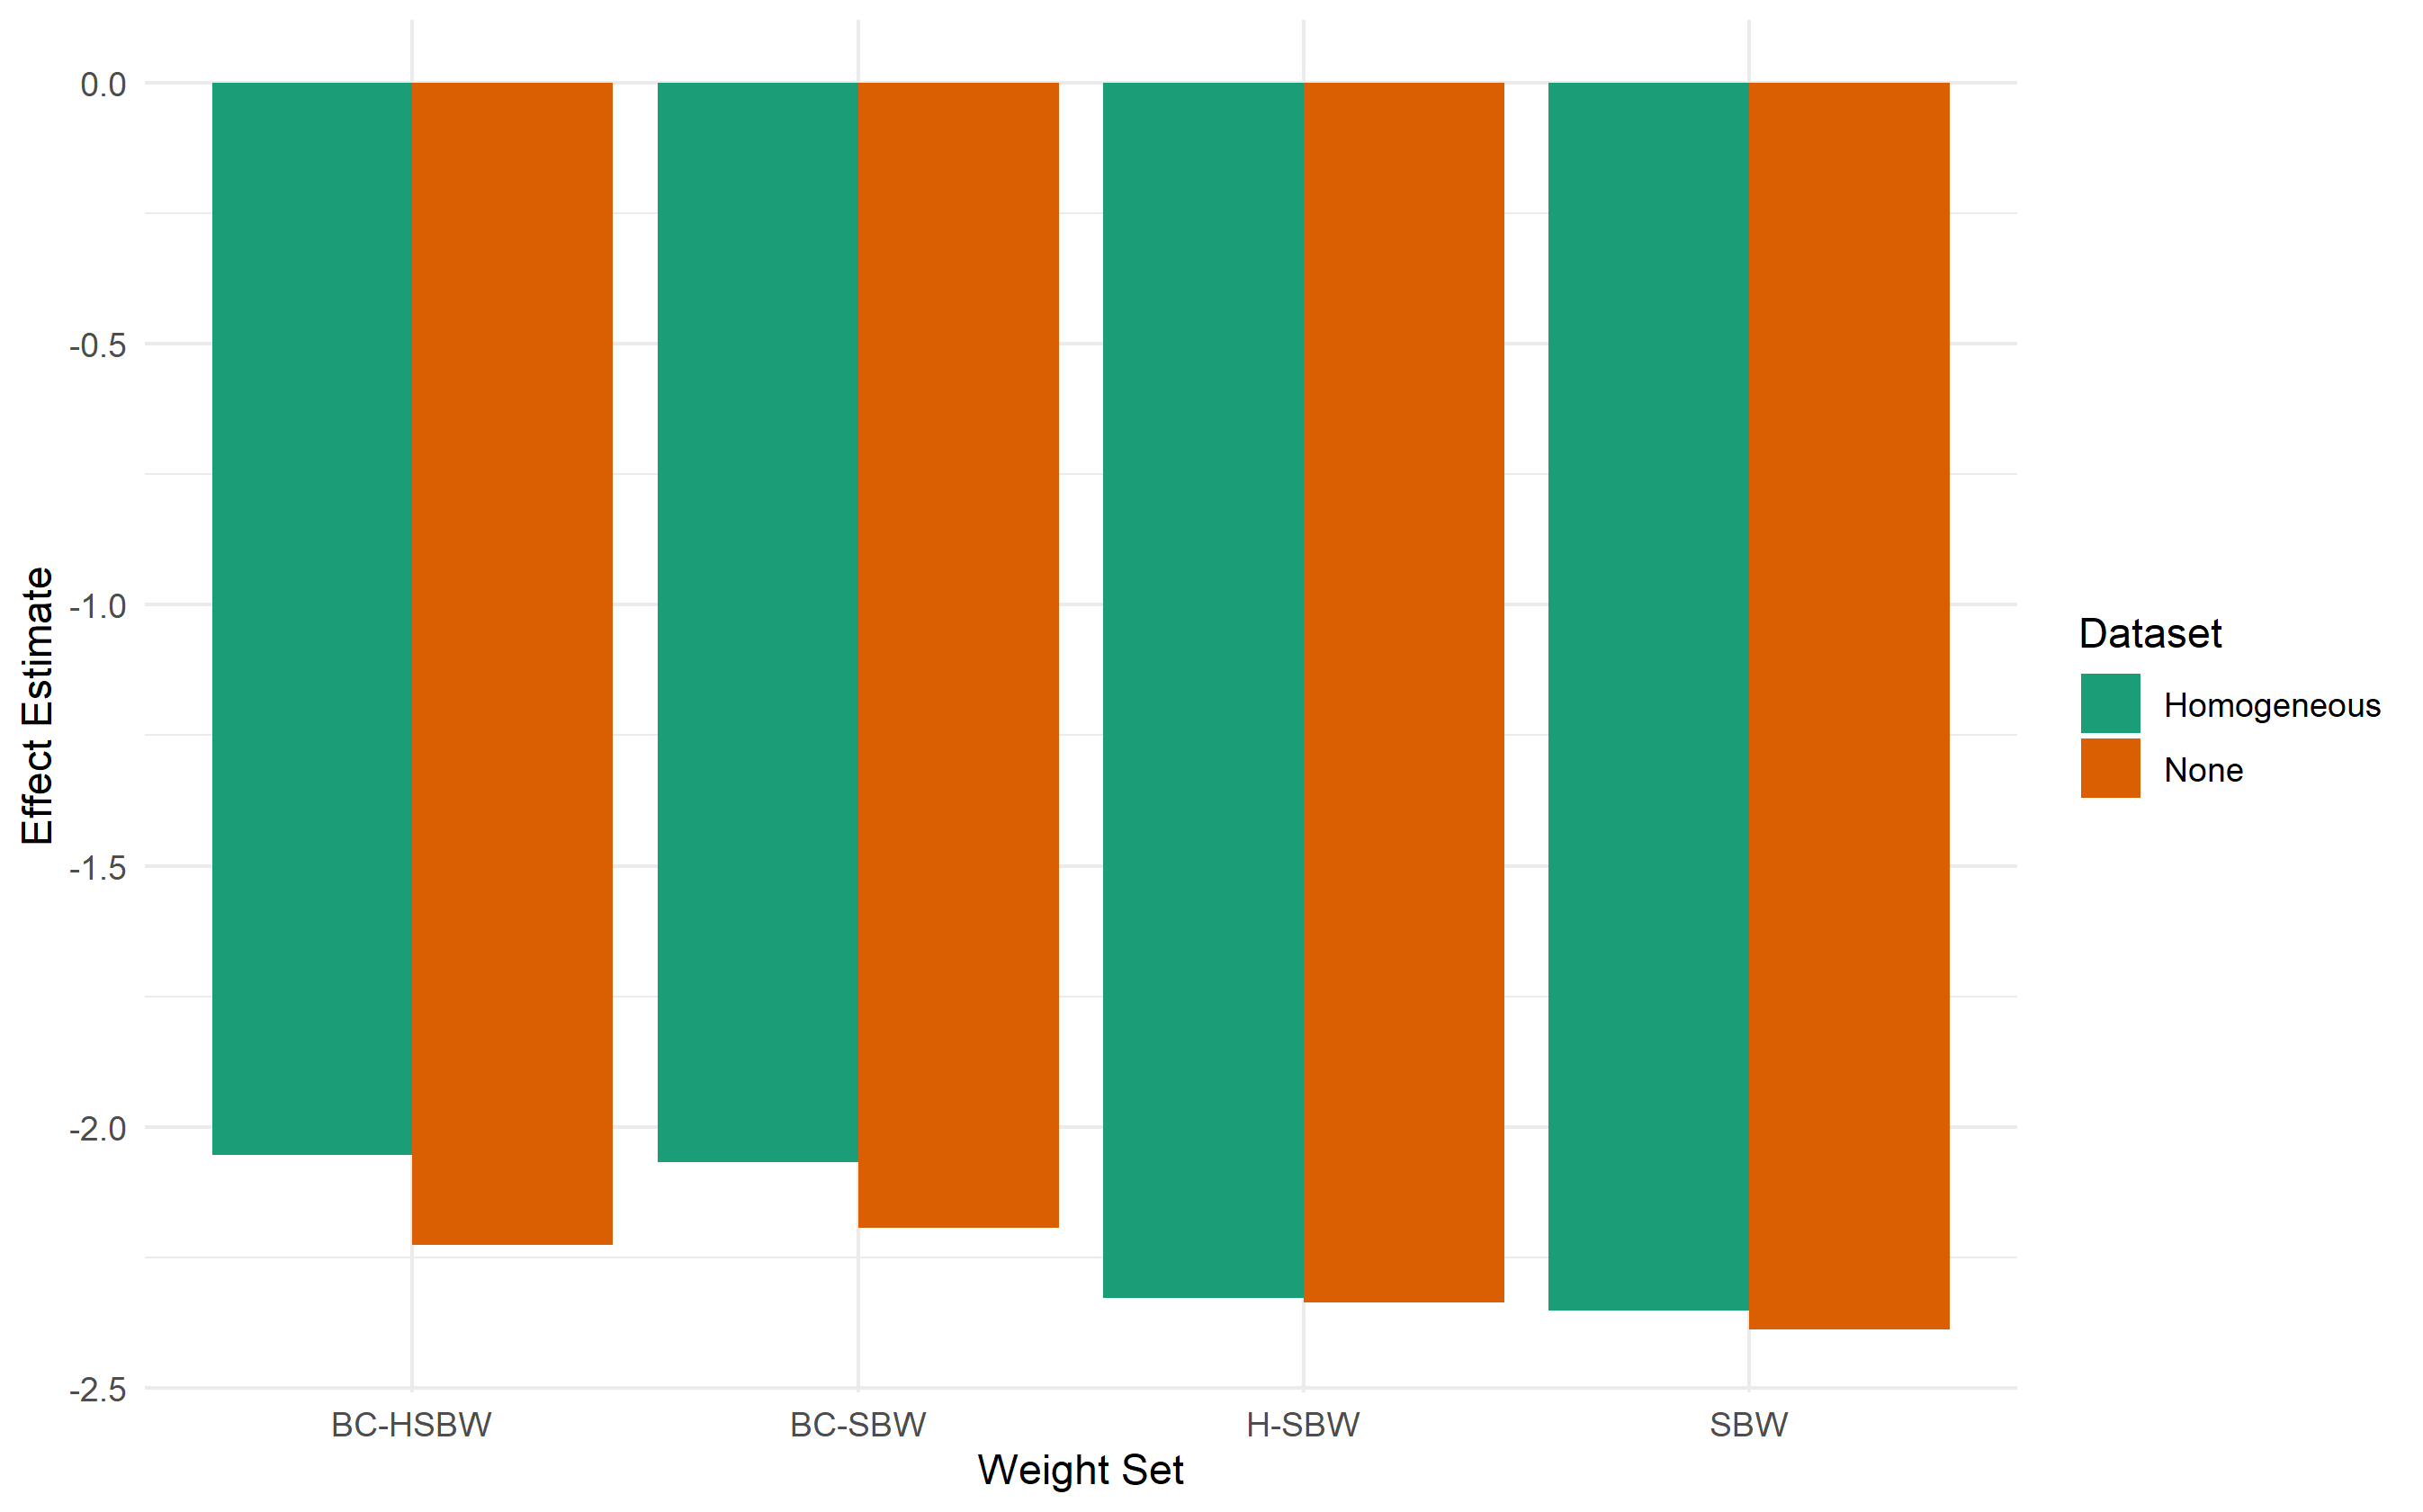
\includegraphics[scale=0.6]{01_Plots/point-estimates-c1.png}
\end{center}
\end{figure}

We examine the robustness of our point estimates to the removal of individual states (note that these are the same point estimates used to calculate our confidence intervals). Figure~\ref{fig:loostateplot} shows how the point estimates change for both the adjusted (``sigma\_uu\_i\_modeled'') and unadjusted (``sigma\_zero'') datasets. We see similar results in either case: removing Ohio tends to decrease the point estimates. By contrast, removing Iowa, Kentucky, or California tends to increase the estimates. The results are quite similar when using an alternative specification for the covariate adjustment and when recalculating the entire procedure. Additional results are available in Appendix E, Table~\ref{tab:loostatec1}. 

\begin{figure}[H]
\begin{center}
    \caption{Estimator sensitivity to states}
    \label{fig:loostateplot}
    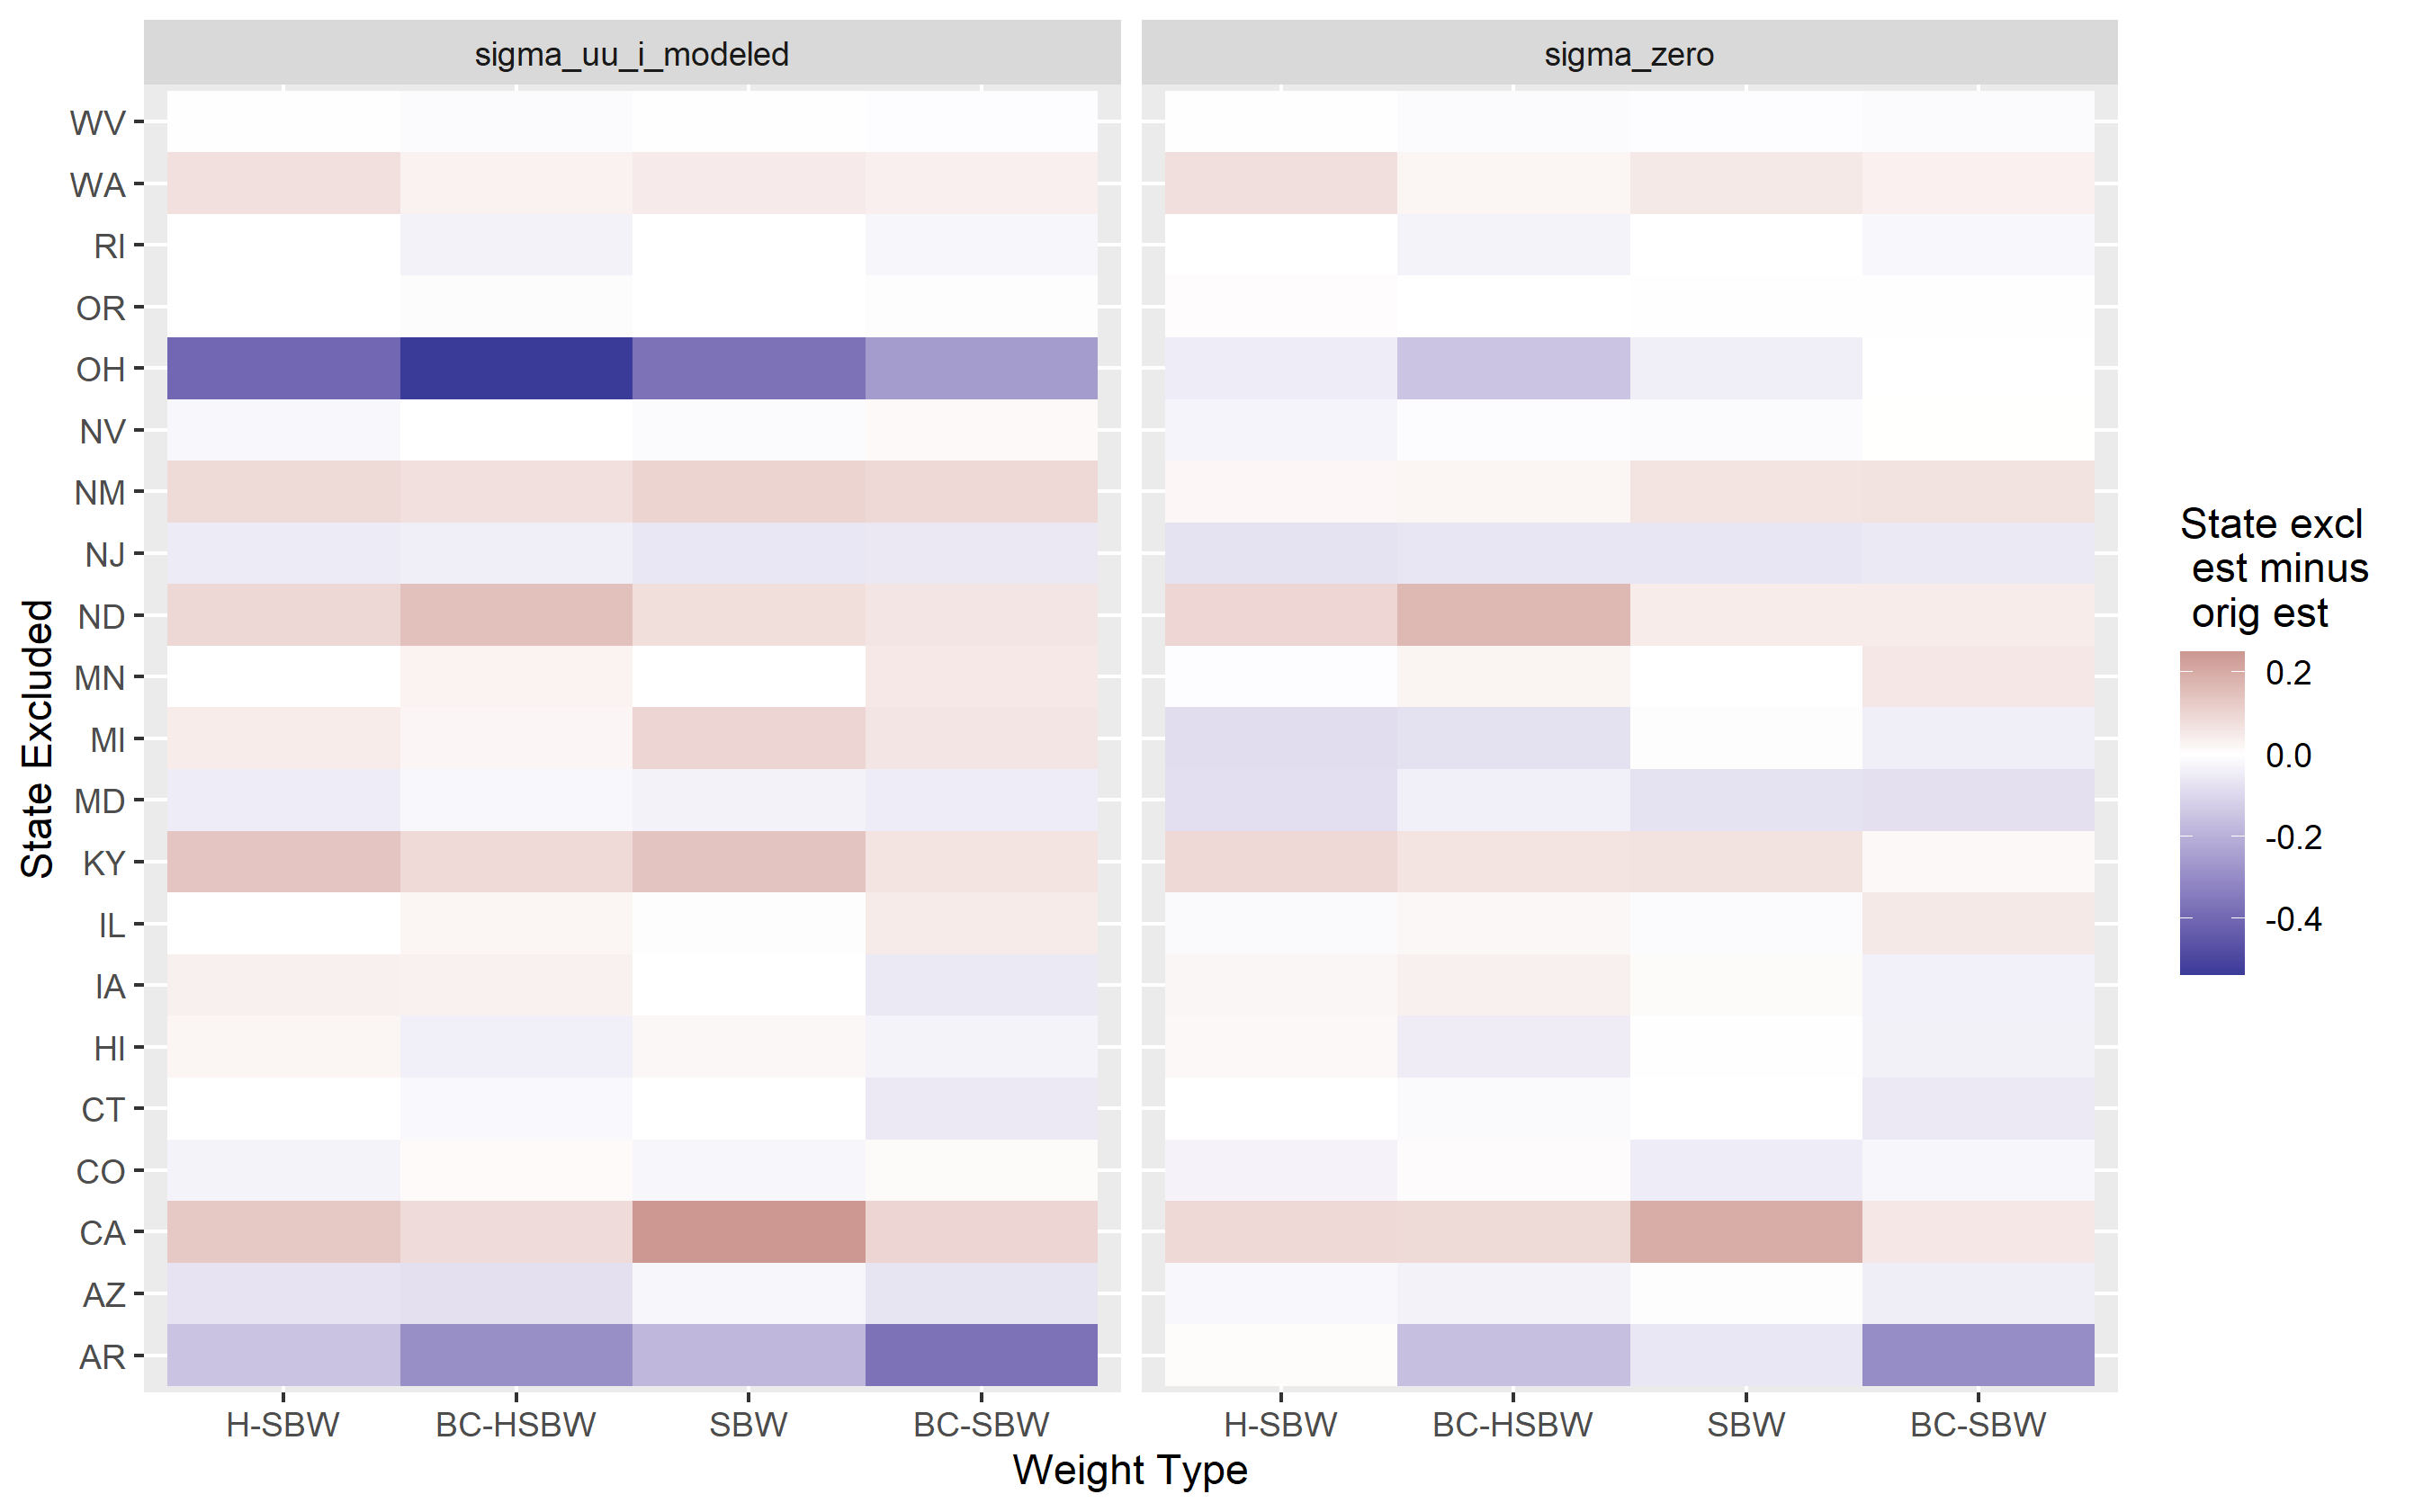
\includegraphics[scale=0.6]{01_Plots/loostate-sensitivityc1-state-uu-i.png}
\end{center}
\end{figure}

Overall we see that our estimates of the ETC are substantially closer to zero than existing estimates of the ETT. We now consider our second research question: whether Republican governance might be driving this apparent difference. As discussed above, due to limited covariate overlap, we restrict this analysis to seeing whether there is an association between our estimated counterfactual outcomes and Republican governance on the treated data. The presence of an association would be consistent, though not definitive evidence, supporting this hypothesis.

Specifically, let $\hat{\Delta}^1$ be the difference in estimates when removing the Republican governance indicators compared to the original estimate. For the H-SBW estimator we calculate $\hat{\Delta}^1$ equal to -0.67 (-1.63, 0.28) for BC-HSBW and -0.74 (-1.86, 0.39). We see similar differentials on our unadjusted dataset (-0.65 (-1.20, -0.09) and -0.70 (-1.48, 0.08), respectively). Interestingly, these contrasts are relatively insensitive to the covariate adjustment procedure. While these confidence intervals often include zero, we find that these differences are negative for all estimators we consider when removing each state. That is, the sign of the differences in the contrasts is negative for every specification that we run.\footnote{When rerunning the entire covariate adjustment procedure, the only specification that is greater than zero occurs for the BC-SBW estimator when removing Illinois. For our secondary adjustment (results available in Appendix E), the BC-SBW results are sensitive to the removal of both Illinois and California and the BC-HSBW to California. None of the leave-one-state-out estimates are greater than zero when removing the early expansion states.} In the context of also calculating a treatment effect much closer to zero than existing estimates of the ETT, we view this as suggestive (though statistically inconclusive) evidence consistent with our research hypothesis.

In Appendix E we also consider four other covariate sets and present these results in Appendix E, Table~\ref{tab:ptests}. None of these results are surprising, though we do see that controlling for pre-treatment outcomes and unemployment rates matters substantially for our point estimates. The other results are slightly sensitive to the removal of different covariate groups, while the changes when removing the pre-treatment unemployment and uninsurance rates or the Republican governance indicators generate the strongest and most consistent contrasts. 

\subsection{Sensitivity Analyses} \label{sssec:sensitivity}

We examine the sensitivity of our analysis to violations of two key causal assumptions: (1) no anticipatory treatment effects, and (2) positivity violations. To the first point, several states had partial limited expansions prior to 2014. Following \cite{frean2017premium}, these states are California, Connecticut, Minnesota, New Jersey, and Washington. We rerun our analyses excluding CPUMAs from all five of these states. It is unclear how removing these states might affect our estimates: on the one hand, states that expanded early might have a smaller treatment effect after 2014 because they already enrolled newly eligible individuals. On the other hand, if these states were also more motivated to enroll people in Medicaid, they might have larger post-expansion coverage gains. Figure~\ref{fig:weightsbystatec2} displays the H-SBW weights summed by state alongside BC-HSBW. We again see that the BC-HSBW estimator extrapolates heavily to reduce the imbalances. A complete balance table is available in Appendix D, Table~\ref{tab:baltab1}.

\begin{figure}[H]
\begin{center}
    \caption{Total weights summed by state, early expansion removed}
    \label{fig:weightsbystatec2}
    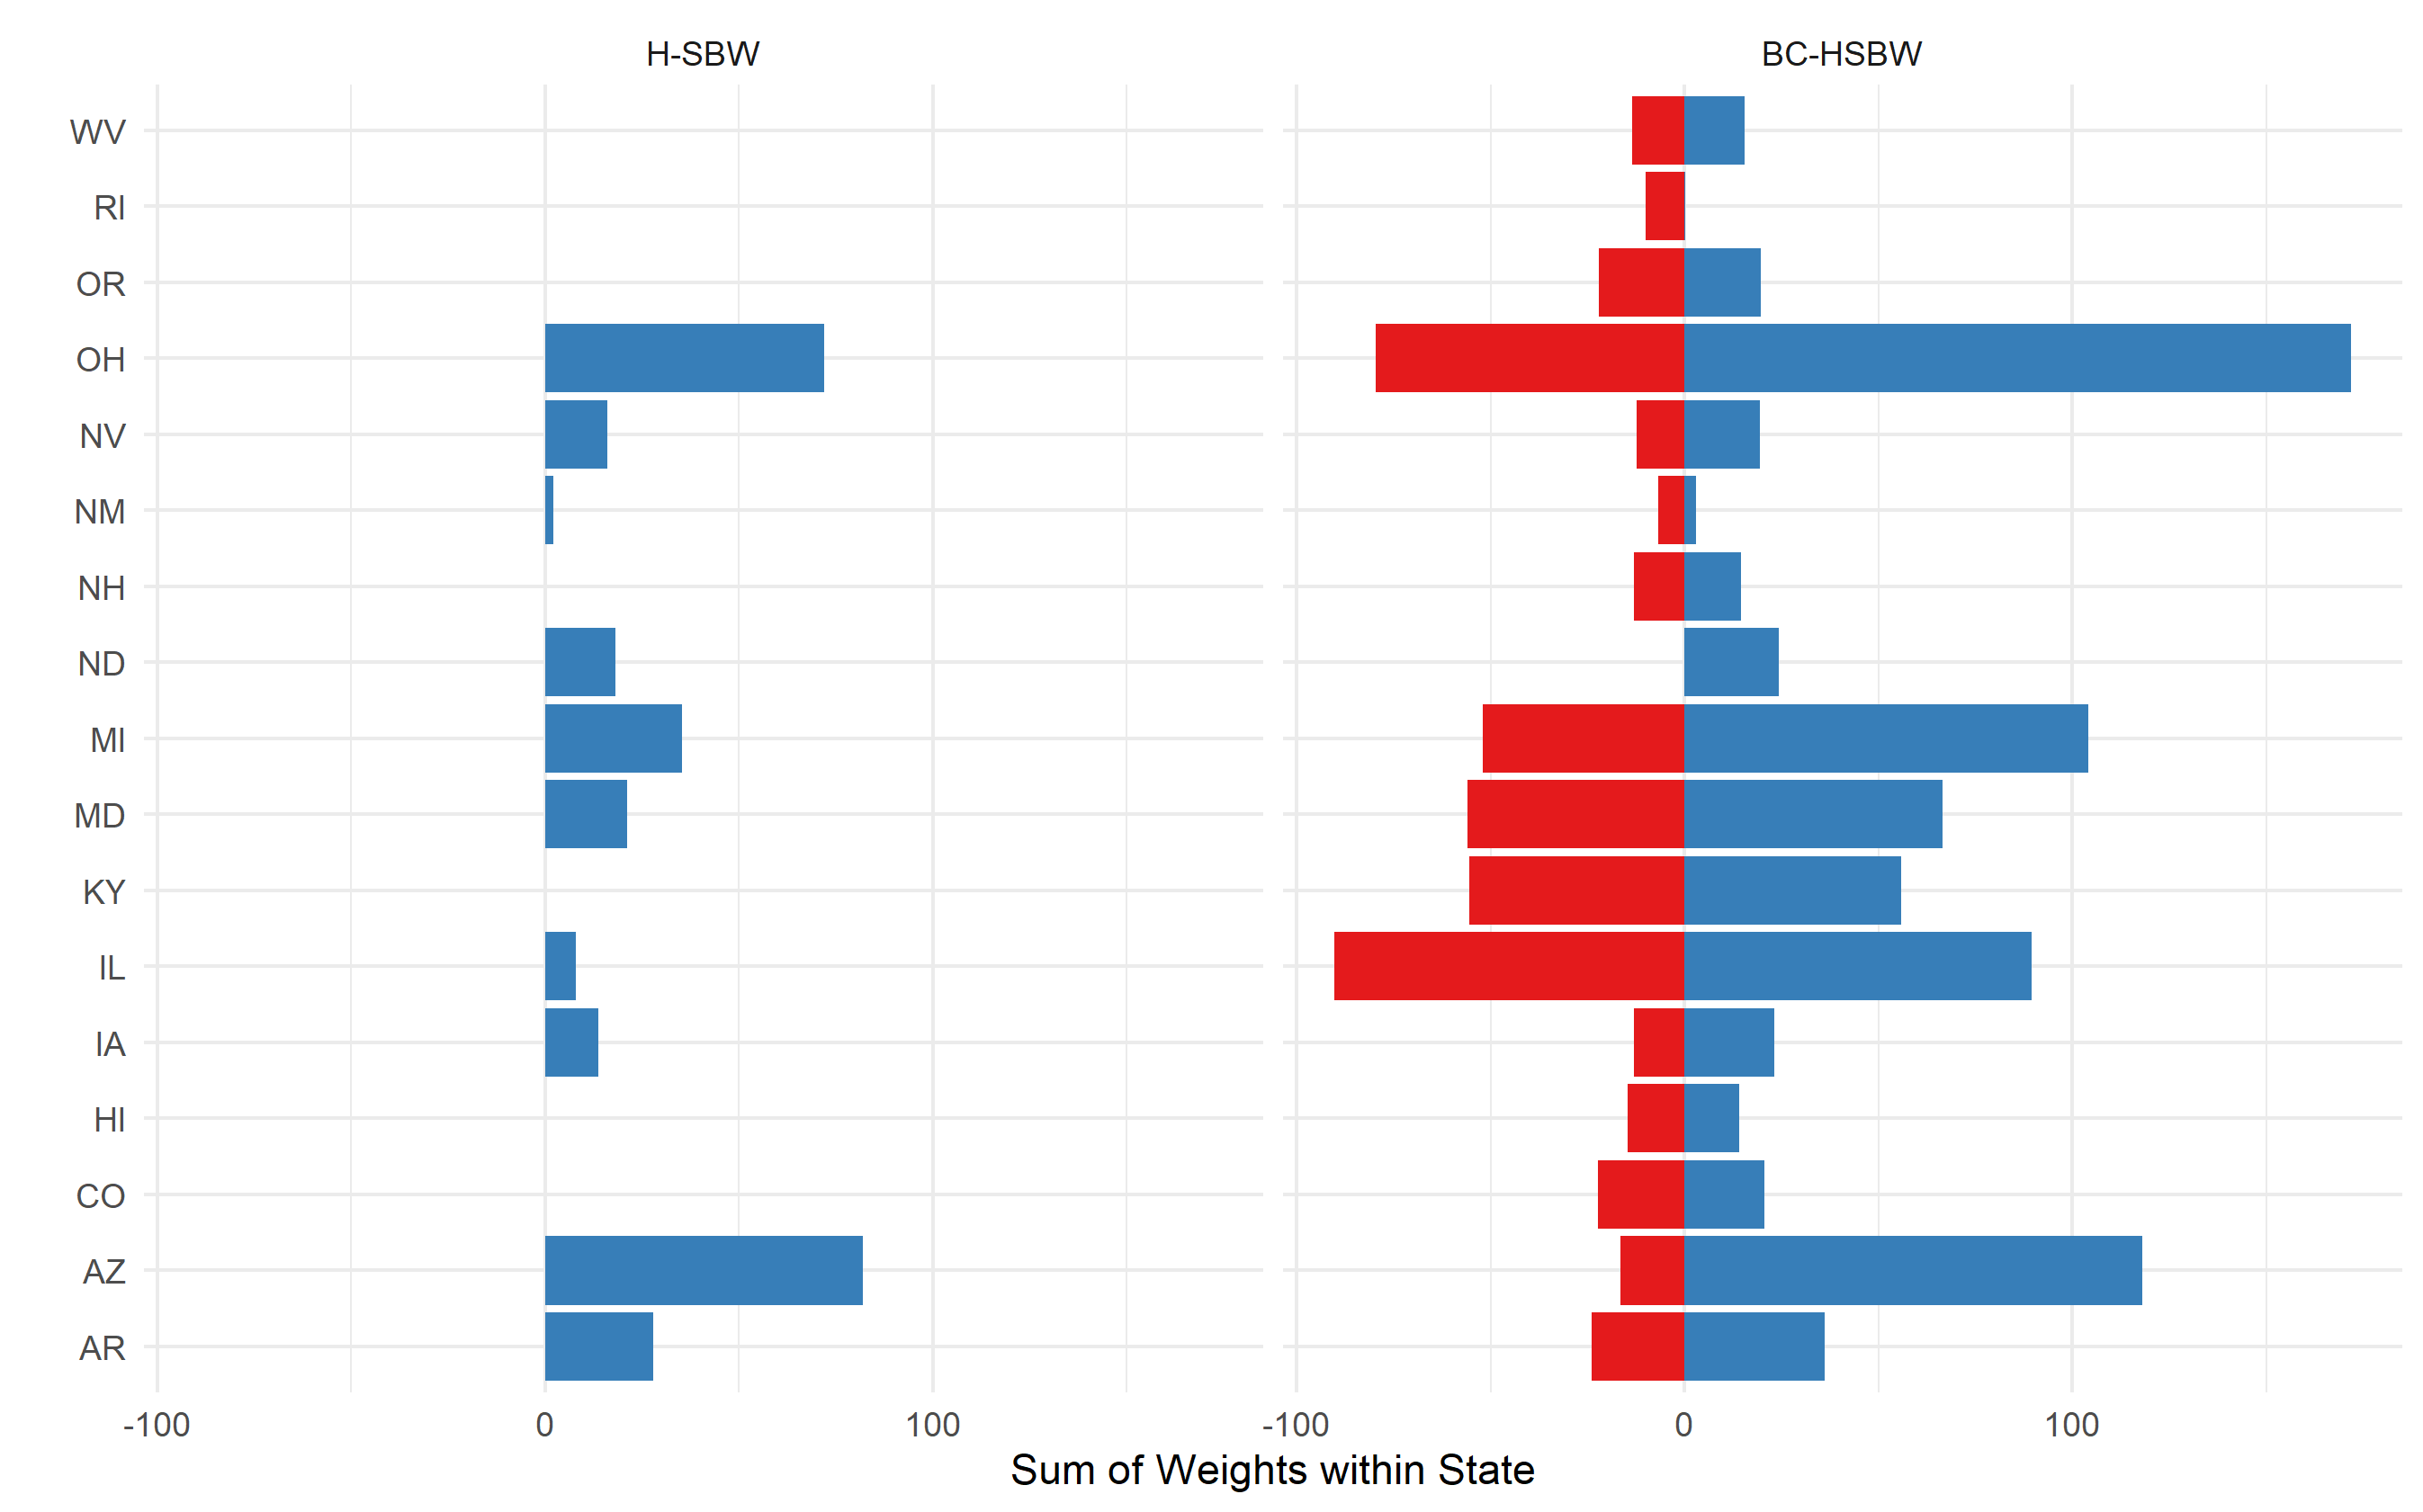
\includegraphics[scale=0.6]{01_Plots/weights-by-state-hsbw-c2.png}
\end{center}
\end{figure}

On this dataset we estimate an effect of -2.04 (-3.10, -1.00) using H-SBW weights; BC-HSBW yields an estimate of -2.13 (-3.63, -0.64). While the point estimate of the H-SBW estimator increases slightly, overall we view this as evidence that our primary point estimates are fairly robust to the exclusion of these states. Table~\ref{tab:confintmainc2} and Table~\ref{tab:secondaryptests} in Appendix E display additional results. 

We also find that our estimates $\hat{\Delta}^1$ decrease slightly. Specifically, we find -0.80 (-1.69, 0.09) percentage point decrease for the H-SBW estimator when excluding the Republican governance indicators and a -0.85 (-2.16, 0.46) increase for BC-HSBW. Figure~\ref{fig:repub} displays these differences in the contrasts against those from our primary dataset. On our unadjusted dataset we estimate contrasts of -0.76 (-1.52, -0.01) and -0.69 (-1.90, 0.52). While these confidence intervals mostly contain zero, we again find that all individual leave-one-out-state out estimates are less than zero. Additional results are available in Appendix E, Table~\ref{tab:deltac2}. 

\begin{figure}[H]
\begin{center}
    \caption{Removing Republican Governance Indicators}
    \label{fig:repub}
    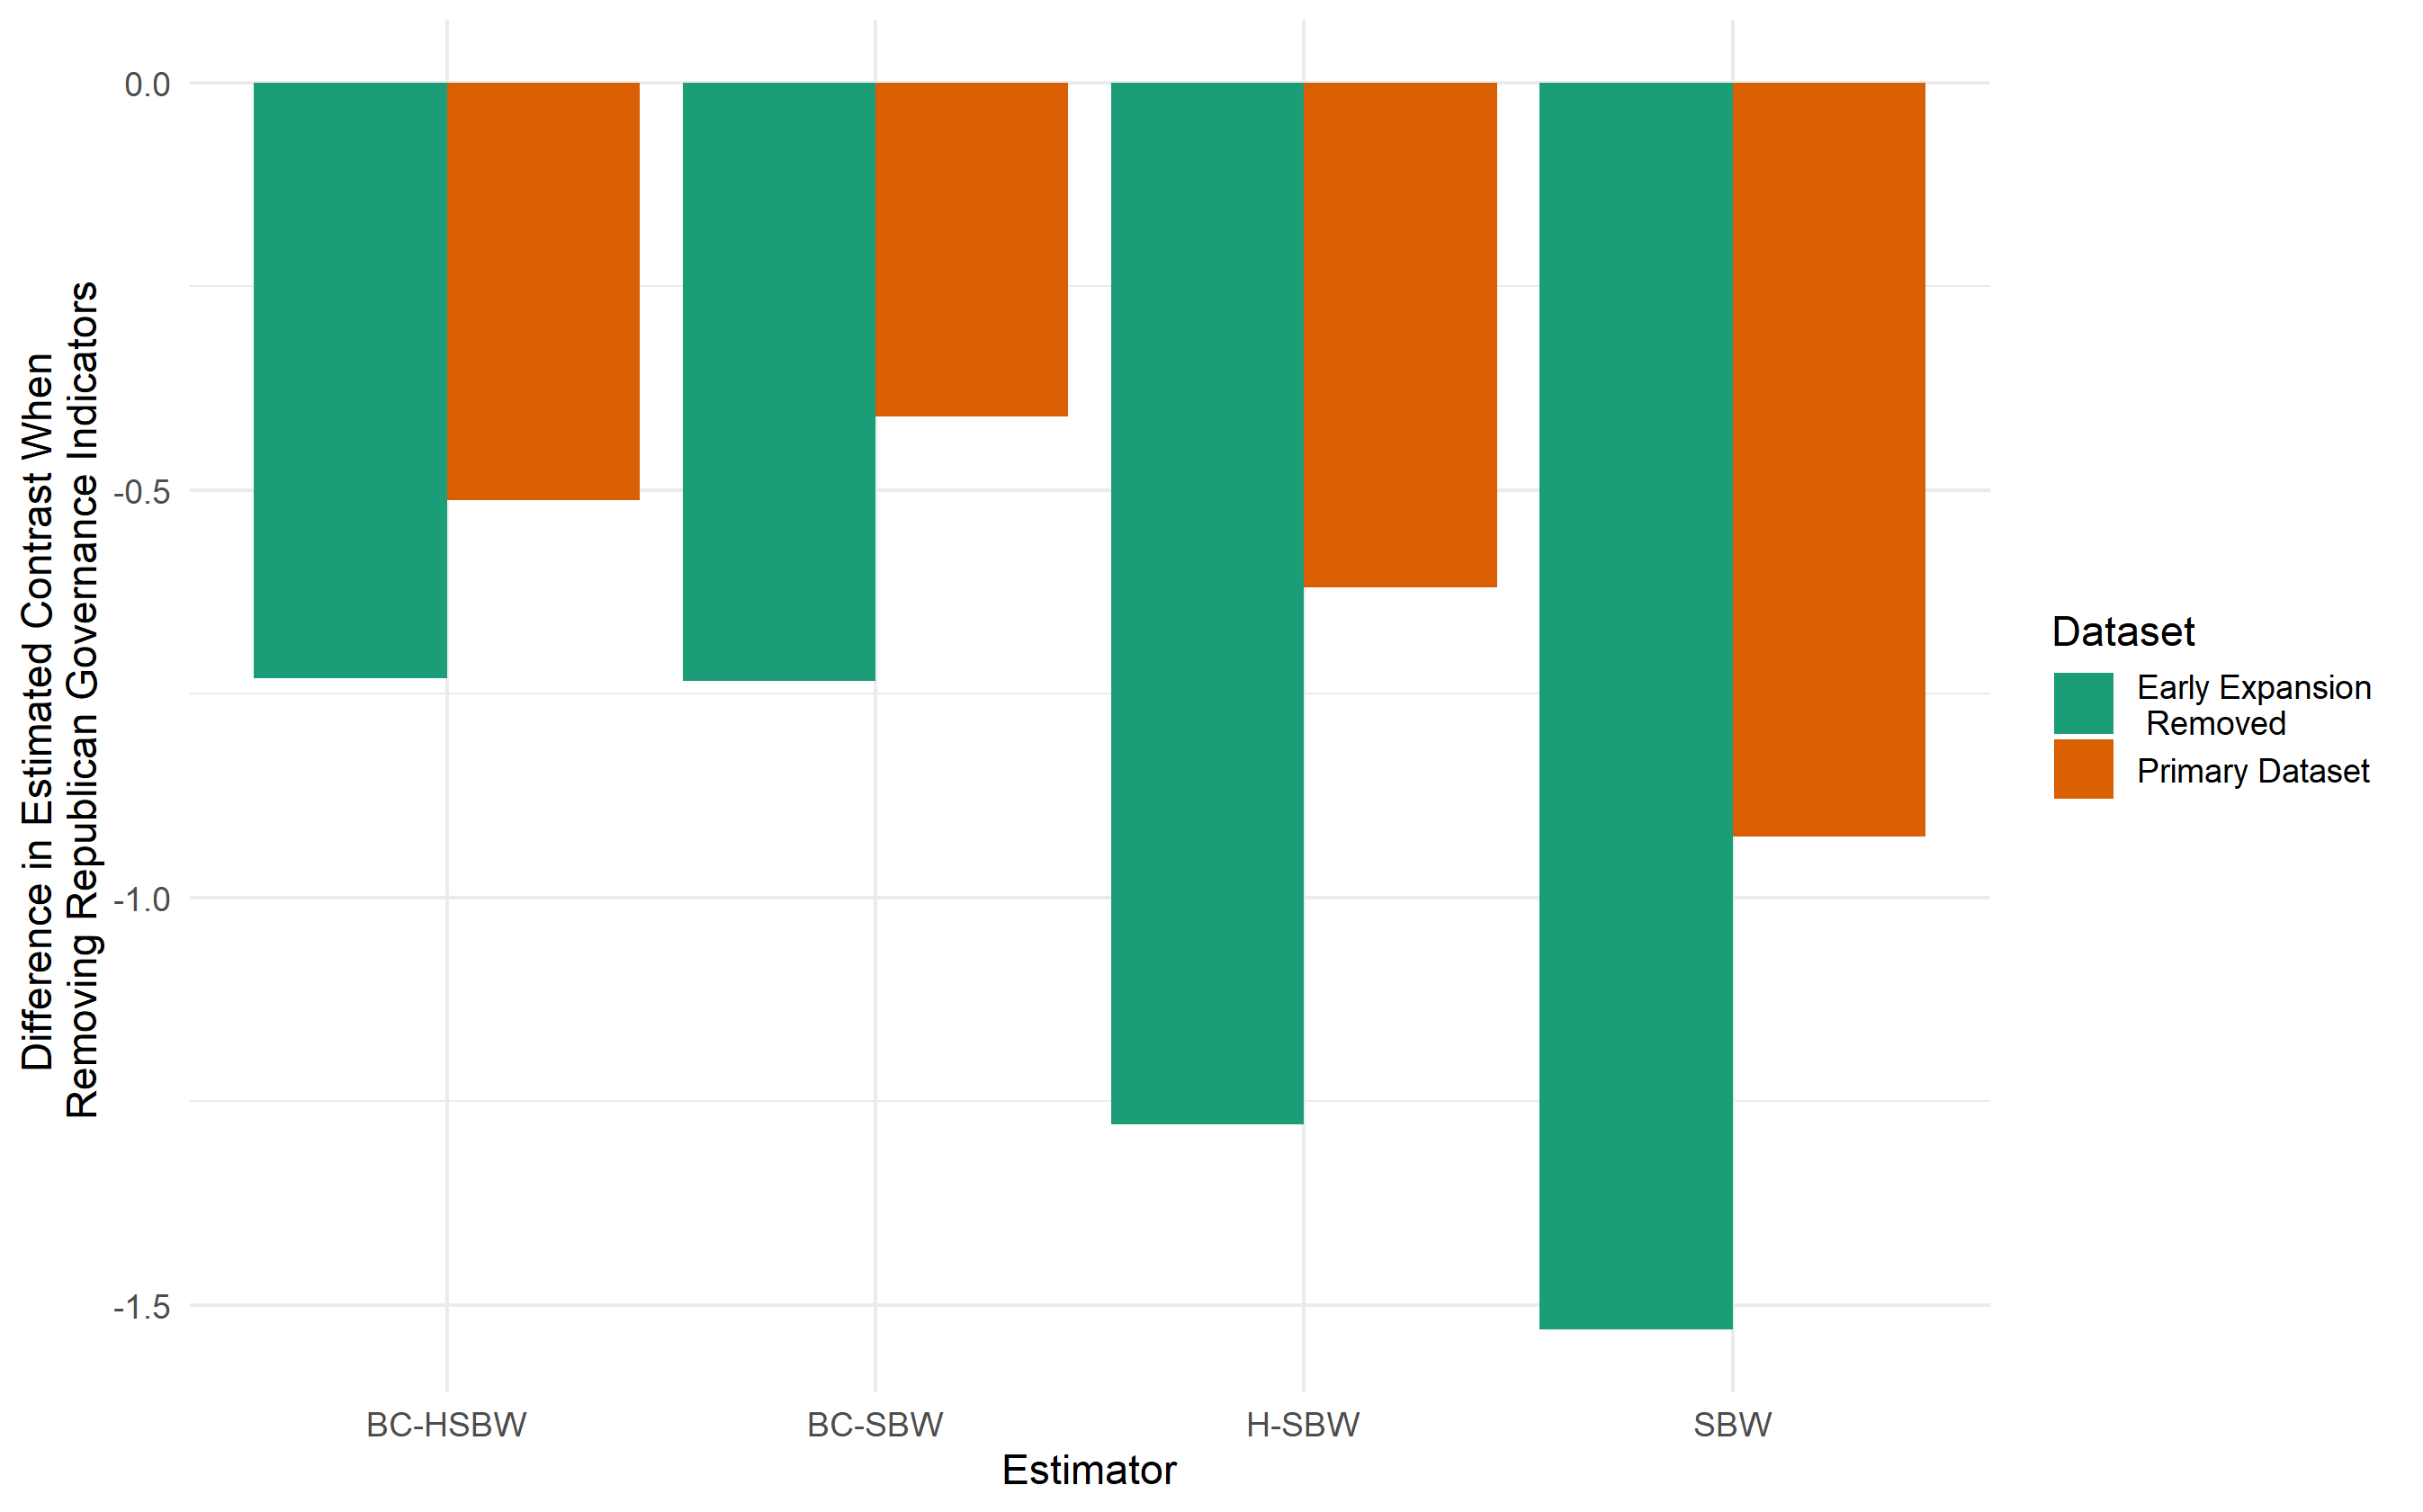
\includegraphics[scale=0.6]{01_Plots/repub-diff-c1c2.png}
\end{center}
\end{figure}

We conclude by considering an alternative method to account for positivity violations. To this point we have relied on either (1) retaining a potentially biased estimate from weights that do not exactly balance the covariates, or (2) producing a more heavily model-dependent estimate that relies on extrapolating beyond the support of the data. Overall we found that the results did not change much either way. Here we consider a third option: changing our target estimand. In particular, we consider the overlap average treatment effect (OATE), proposed by \cite{li2018balancing}. This is the treatment effect on the subset of the entire dataset where we have overlap. It is a data-dependent treatment effect, and is not the same as the ETC; however, we believe that this effect will be more similar to the ETC than the ETT, particularly because there were no Democratic controlled states that did not expand Medicaid. After generating overlap weights on our primary dataset we find that across all covariates, the mean average absolute distance from the overlap region to the untreated region is 2.24 and to the treated region is 7.55.\footnote{This distance is calculated on the adjusted dataset. When excluding early expansion states the distance is 2.21 to the untreated and 5.19 to the treated region.} Figure~\ref{fig:oateimbalance} displays the distance between covariates with greater than one percentage point distance from the overlap region to either the control or treated region. We see that the overlap region is substantially more Republican than the treated region, as expected. This region is also less Hispanic, more white, less rural, and more educated than either the expansion or non-expansion region. Table~\ref{tab:oatedist1} and Table~\ref{tab:oatedist2} in Appendix D show additional statistics on the OATE region versus the treatment and control regions for all covariates.

\begin{figure}[H]
\begin{center}
    \caption{Overlap area compared to treated, untreated regions}
    \label{fig:oateimbalance}
    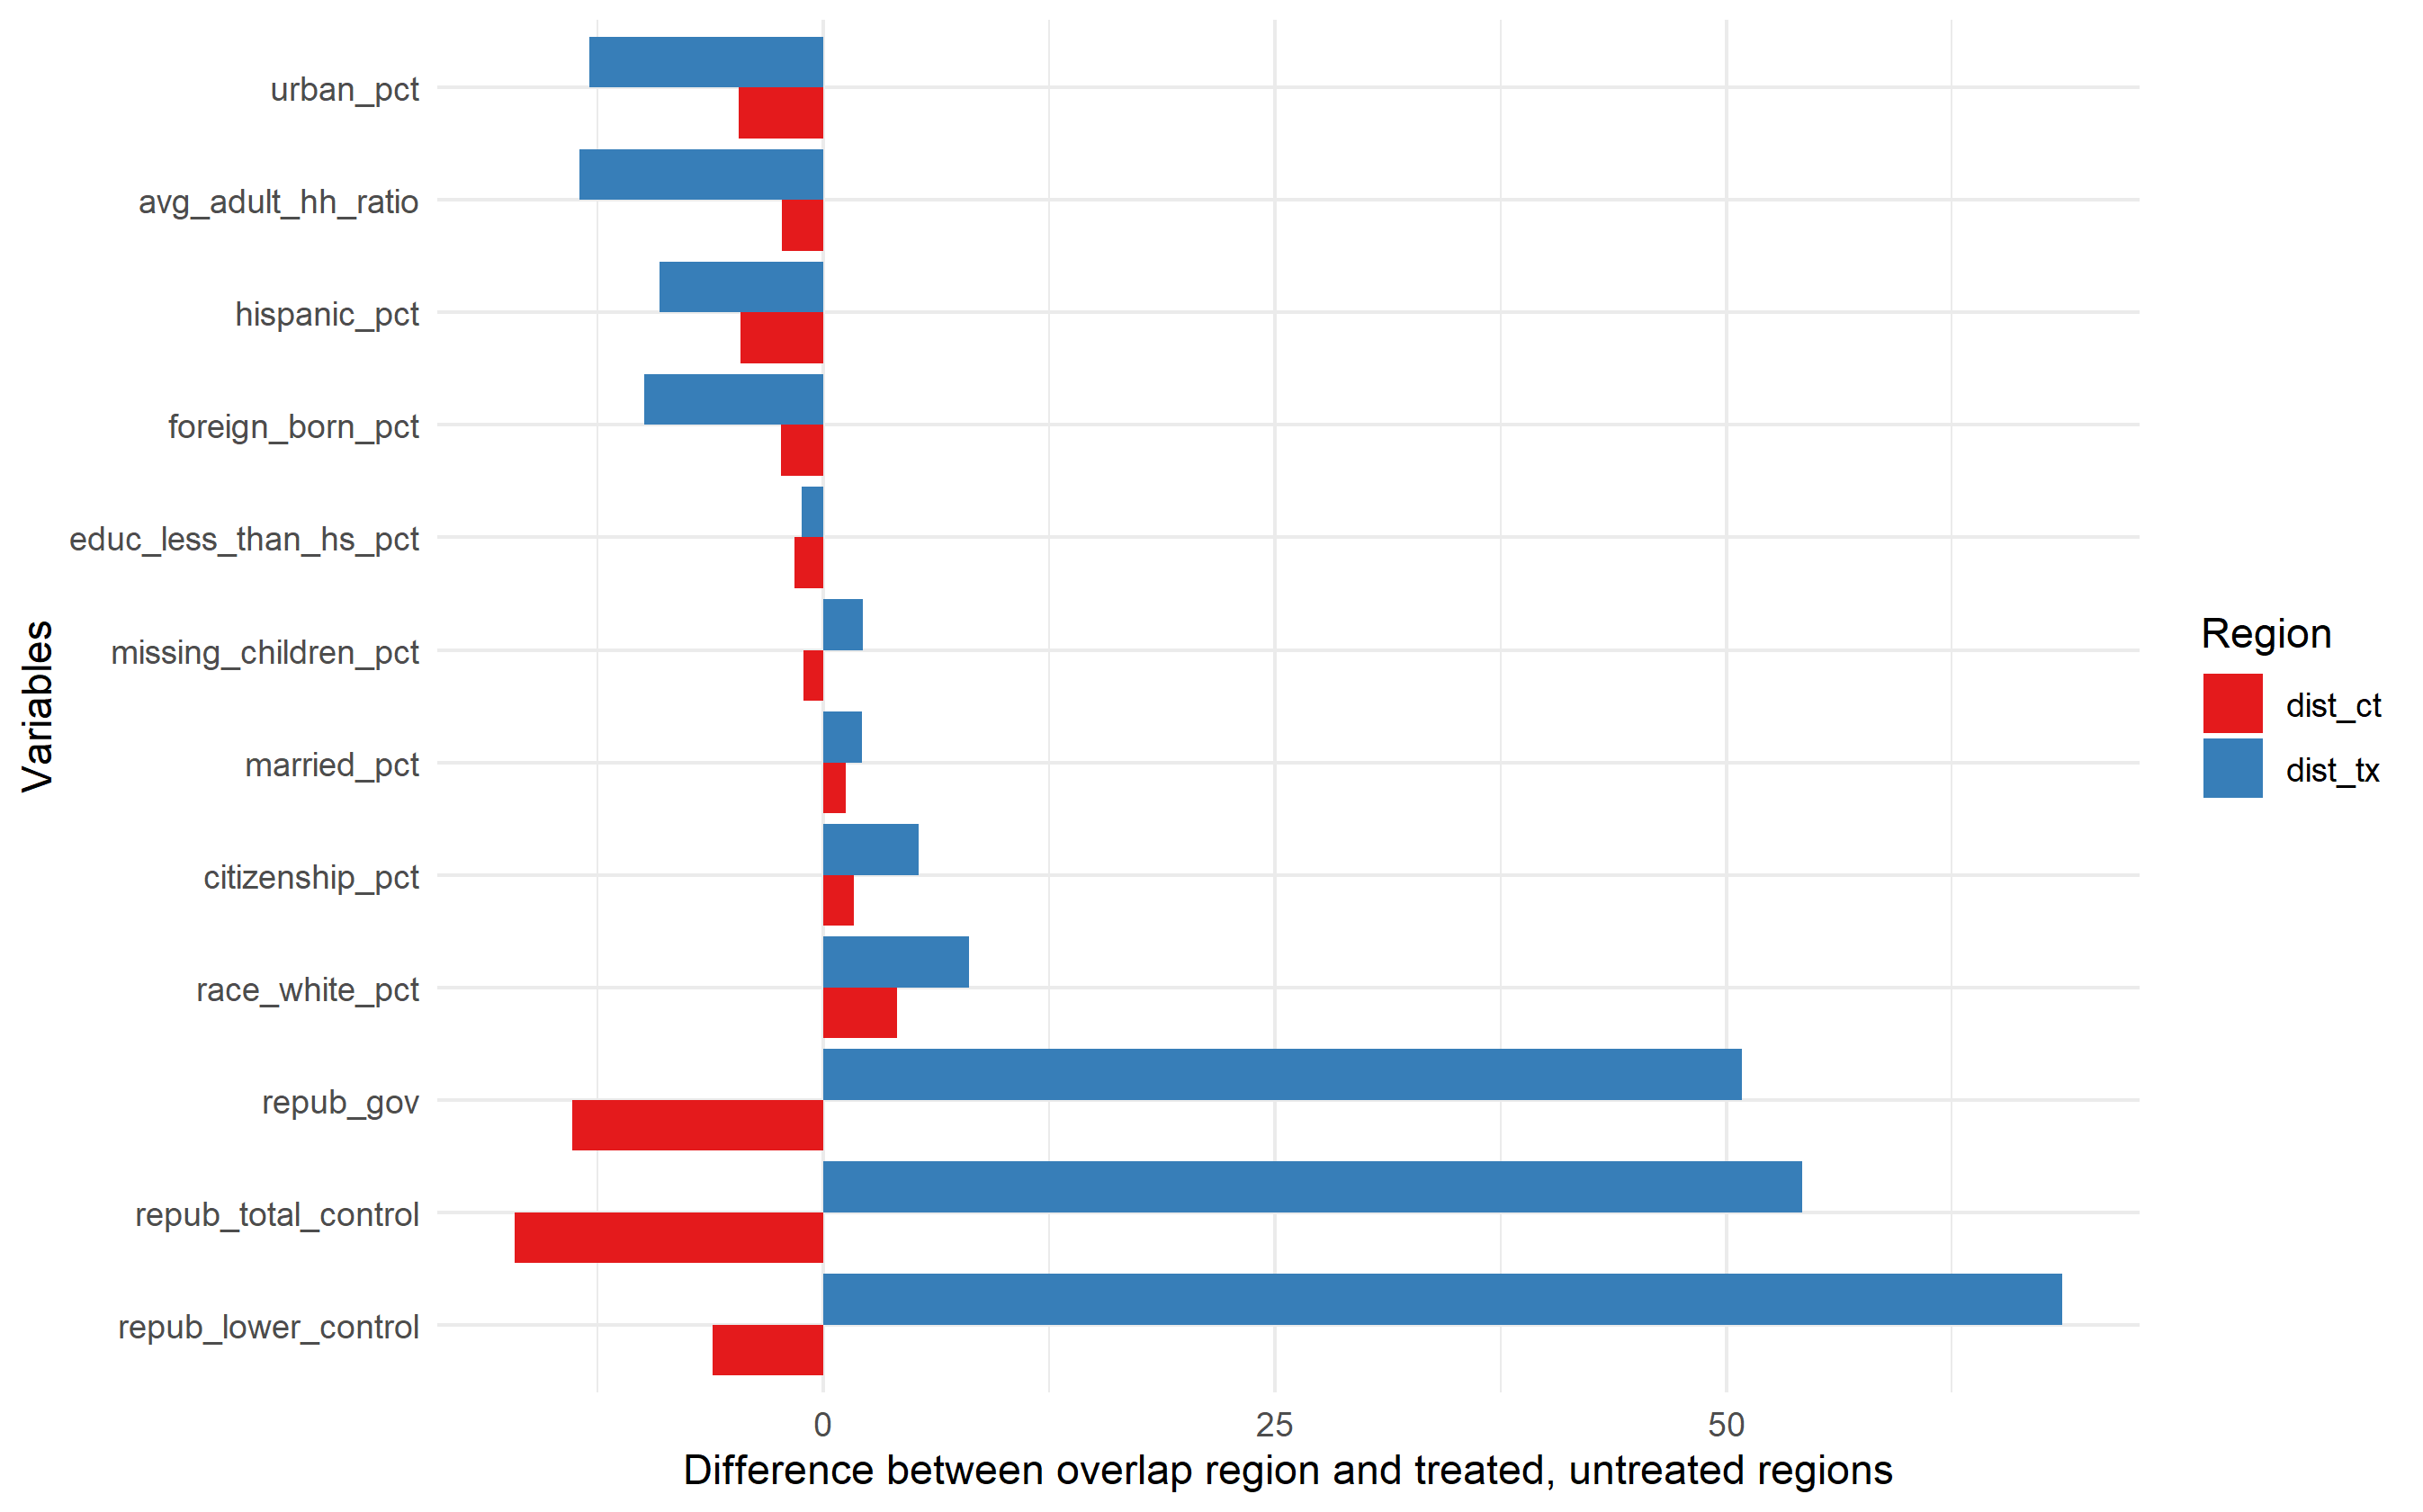
\includegraphics[scale=0.6]{01_Plots/oate-imbalances-c1.png}
\end{center}
\end{figure}

Figure~\ref{fig:oateimbalance} displays the sum of the weights within each state by treatment group. California, Ohio, and Oregon, which all expanded Medicaid, are the most heavily weighted states (the weights are standardized within each treatment group to sum to 100). The weights are more evenly dispersed among the non-expansion regions, though Alabama, Florida, Wisconsin, and Pennsylvania are given the most weight. We note that this region is specific to the preferred covariate adjustment; the results are quite similar for the unadjusted and less preferred covariate adjustment and are available in Appendix D, Table ~\ref{tab:oatestateweights}.

\begin{figure}[H]
\begin{center}
    \caption{Overlap weights by state}
    \label{oatearea}
    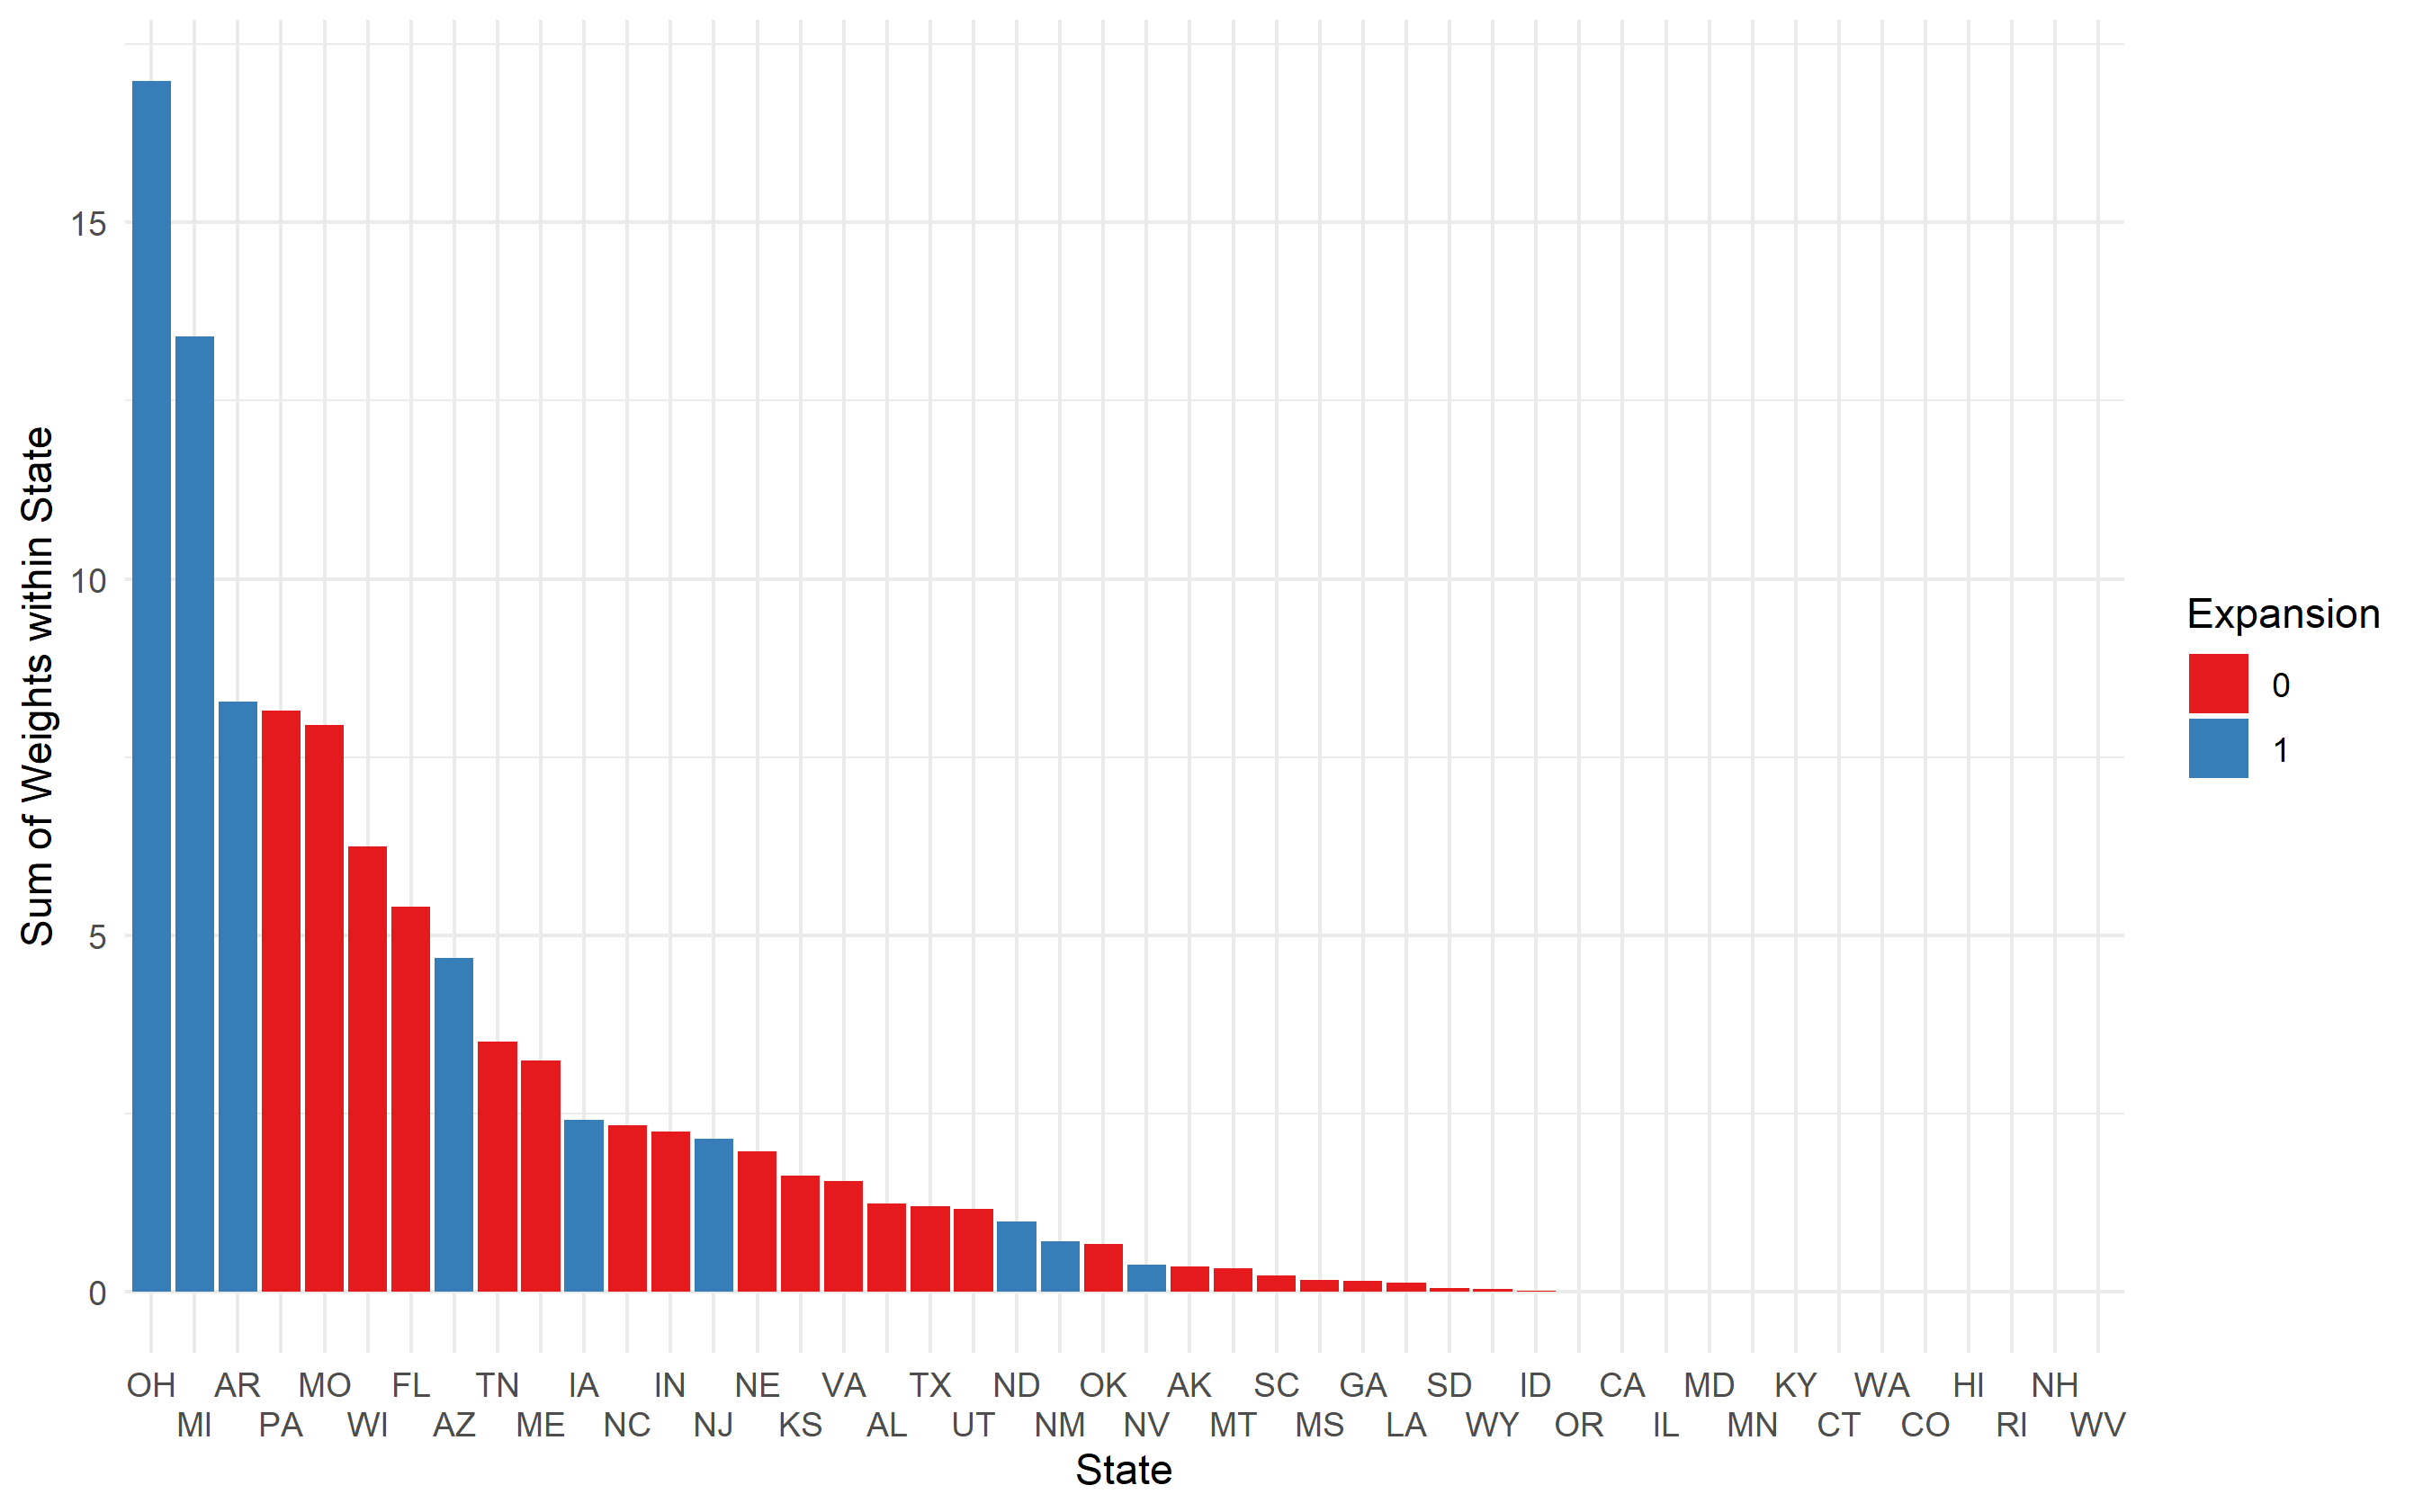
\includegraphics[scale=0.6]{01_Plots/oate-region-c1-a.png}
\end{center}
\end{figure}

The point estimates are somewhat larger relative to our primary analysis: within the overlap region we estimate a treatment effect -1.74 (-2.35, -1.14) when including all treatment states in our primary analysis, and of -1.89 (-2.47, -1.32) when excluding the early expansion states. Moreover, these results are quite similar compared to the unadjusted datasets: -1.80 (-2.50, -1.10) on the primary dataset and -1.95 (-2.65, -1.25) when excluding early expansion states. 

We again find a negative contrast when comparing an estimate excluding the Republican governance indicators against our primary estimate: however, we caveat that unlike the previous analysis, this difference is a function of the differences in the weighted covariates among both the treated and control regions, and does not attempt to hold the other imbalances fixed at any particular quantity. Regardless, this estimate can inform us about the association between Republican governance and the overlap average treatment effect. We find that the estimate changes by -0.90 (-1.09, -0.70) percentage points on the primary dataset and by -0.67 (-0.90, -0.44) percentage points when removing early expansion states. These differences are statistically significant; moreover, this negative difference in estimated contrasts holds for each excluded state. Additional results are available in Appendix E, Table~\ref{tab:oateconfint} and Table~\ref{tab:oatesensitive}. 

\section{Discussion}

We estimate that had states that did not expand Medicaid in 2014 instead expanded their programs, they would have seen a -2.17 (-3.41, -0.94) percentage point change in the adult uninsurance rate. Existing estimates place the ETT between -3 and -6 percentage points; these estimates vary depending on the targeted sub-population of interest, the data used, and the modeling approach (see, e.g., \cite{courtemanche2017early}, \cite{kaestner2017effects}, \cite{frean2017premium}). This ETC estimate is therefore closer to zero than these ETT estimates, supporting our original hypothesis that the treatment effect on non-expansion states would be smaller in absolute magnitude. Moreover, we also find suggestive, though statistically inconclusive, evidence that factors associated with Republican governance may drive this differential. 

We also make several methodological contributions to the literature on balancing weights. First, we extend the synthetic controls literature to estimate the treatment effect on the controls. The key challenge is that we need to predict treatment response rather than the outcome absent treatment. Unlike when estimating the treatment effect on the treated, we cannot use pre-treatment outcomes to conduct variable selection, run placebo tests, or train our model in some other way. This is a fundamentally more difficult problem that requires greater modeling assumptions. Second, we extend the Stable Balancing Weights objective function for use with hierarchical data and covariates measured with error. We modify the criterion to more evenly disperse the weights across states, and the constraint set to balance on a linear approximation to the true covariate values using regression-calibration techniques (\cite{gleser1992importance}).

Our study's approach also has bearing on estimating and understanding the ETT using a difference-in-differences design. If we believe that Republican governance is associated with changes in trends over time, then we need to control for this factor. However, there is likely insufficient overlap to control for governing ideology without significantly extrapolating from the data. We see that the ETC requires less extrapolation than the ETT with respect to governance, and therefore requires less model-dependent estimates.

Finally, our results caution against using estimates of the ETT to make inferences about the ETC. Because almost every outcome of interest is largely mediated through increasing the number of insured individuals, and because we have shown that our estimate of the ETC is somewhat closer to zero than existing estimates of the ETT, projecting findings from an estimate of the ETT to the ETC may lead to inaccurate inferences. For example, \cite{miller2019medicaid} study the effect of Medicaid expansion on mortality. Using their estimate of the ETT they project that had all states expanded Medicaid, 15,600 deaths would have been avoided during their study's time-period. If we believe that this number increases monotonically with the number of uninsured individuals, then our results suggest this projection may be an overestimate. Directly estimating the ETC can therefore also help us better model interesting downstream effects mediated through decreasing the uninsurance rate. 

We conclude by discussing the policy implications of these findings. First, a reduction of adult uninsurance rates by -2.17 percentage points represents an 11 percent reduction in the uninsurance rate among non-expansion states. As observed previously, this estimated treatment effect is closer to zero than corresponding estimates of the ETT (see, e.g., \cite{courtemanche2017early}), and we may therefore expect that downstream effects that move away from zero monotonically with the number of uninsured are also closer to zero than estimates of the ETT. Second, to that extent that we believe this association we find in this study, we caution that this is simply an association. This does not imply, for example, that states with more conservative governments deliberately make Medicaid enrollment more difficult relative to Democratic states. As \cite{sommers2012understanding} notes, people may be less likely to enroll in Medicaid in conservative states due to social stigma and/or personal beliefs about the welfare state. Regardless of the true cause, to evaluate the policy implications of this finding, we compare this result against Congress's goal in implementing Medicaid expansion in the 2010 ACA, which was to improve health insurance access and coverage. Measured against this intent, federal policies may wish to encourage states to make Medicaid enrollment easier, for example, by making enrollment automatic. 

\section{Conclusion}

This is the first study to directly estimate the foregone coverage expansions of Medicaid expansion on states that did not expand Medicaid in 2014. Our estimation approach contributes to the methodological literature on synthetic controls by clarifying the assumptions required to use longitudinal data to estimate the ETC rather than the ETT, and to the balancing weights literature more generally by considering the case where we have hierarchical data and covariates measured with error. We estimate that had states that did not expand their Medicaid eligibility requirements in 2014 done so, they would have seen a -2.17 (-3.41, -0.94) percentage point change in their uninsurance rate. This is substantially closer to zero than existing estimates of the ETT, which range between -3 and -6 percentage points. We hypothesize that Republican governance might drive this heterogeneity, and we investigate this by examining the relationship between Republican governance and the uninsurance rate among the expansion states. We find a positive, though statistically insignificant, relationship, although we find that the sign of this relationship is robust across almost all of our modeling specifications. Were this association true, it may explain this difference, and would be consistent with the previous finding that Medicaid take-up rates are lower in Republican-governed states prior to Medicaid expansion in 2014 (\cite{sommers2012understanding}). From a practical standpoint, our results suggest that we should be cautious about using existing estimates of the ETT to make inferences about the ETC. From a policy standpoint, if the goal of Medicaid expansion is to increase access to insurance for low-income adults, state and federal governments may wish to consider policies that make enrollment in Medicaid easier.

%%%%%%%%%%%%%%%%%%%%%%%%%%%%%%%%%%%%%%%%%%%%%%
%% Single Appendix:                         %%
%%%%%%%%%%%%%%%%%%%%%%%%%%%%%%%%%%%%%%%%%%%%%%
%\begin{appendix}
%\section*{???}%% if no title is needed, leave empty \section*{}.
%\end{appendix}
%%%%%%%%%%%%%%%%%%%%%%%%%%%%%%%%%%%%%%%%%%%%%%
%% Multiple Appendixes:                     %%
%%%%%%%%%%%%%%%%%%%%%%%%%%%%%%%%%%%%%%%%%%%%%%
\begin{appendix}

\import{Text_files}{/proof}

\section{Summary Statistics and Covariates}\label{app:sumstats}

In this section we display summary statistics about the CPUMA-level datasets. The first two tables pertain to treatment assignment classifications. Table~\ref{tab:txassign} lists the states that are assigned to each group: the first two columns include the treatment states and control states in our primary analysis. The third column lists the treatment states for our sensitivity analysis that excludes ``early expansion'' states. The final column indicates states that were always excluded from the analysis. Table~\ref{tab:cpumasperstate} displays the total number of CPUMAs per state, as well as a column reiterating the state's treatment assignment and whether it was an early expansion state.

The subsequent tables and figure display summary information about the expansion state data and the homogeneous and heterogeneous covariate adjustments detailed in Appendix~\ref{app:adjustmentdetails}. 

Table~\ref{tab:summarytab1} displays univariate summary statistics for the treated CPUMAs. Specifically, the table displays mean, interquartile range, and the range (as defined by the maximum value minus the minimum value) for the unadjusted dataset, the heterogeneous adjustment, and the homogeneous adjustment. We see that the covariate adjustments generally reduce the variability relative to the unadjusted data. 

Table~\ref{tab:extreme1} displays the frequency that the adjusted covariates fell outside of the support of the unadjusted dataset on our primary dataset. The frequency is comparable for either adjustment and the counts are low, supporting the use of the linear model outlined in \eqref{eqn:regcal}. We also calculate these adjustments excluding early expansion states, and recalculate these adjustments excluding each state one at a time to calculate our variance estimates, yielding different results with respect to the quality of the resulting adjustments. These results are available on request.

Table~\ref{tab:timetrends} displays the trends in the outcome over time by treatment group. We use these estimates to compute the difference-in-differences estimator of the ETT in footnote \ref{footnote_did}. 

Figure~\ref{fig:corrmatrix} displays the Pearson's correlation coefficients for the bivariate relationships between the covariates on the unadjusted dataset (including both treated and untreated units). These point estimates may be biased due to the measurement error in the covariates. Nevertheless, this matrix is useful for at least two reasons: first, assuming the correlations among the treated and untreated units are similar, the more heavily correlated the data the easier it should be to attain covariate balance (see, e.g., \cite{d2021overlap}). This matrix gives a general sense of how correlated the data are, even if the estimates are biased. Second, these correlations can suggest potential confounders by revealing which variables are most heavily associated with treatment assignment and the pre-treatment outcomes. For example, the plot shows a strong association between Republican governance and treatment assignment, and a smaller association between these variables with pre-treatment outcomes. The plot also illustrates strong associations between the pre-treatment uninsurance rates, though they are more weakly associated with treatment assignment. 

\begin{table}[h!]\caption{Treatment assignment classification}\label{tab:txassign}
\centering
\hline 
\begin{tabularx}{\textwidth}{XXXX} \\ 
Treated states & Control states & Early expansion states & Always excluded \\ 
\hline
AR, AZ, CA, CO, CT, HI, IA, IL, KY, MD, MI$^\textrm{a}$, MN, ND, NJ, NM, NV, OH, OR, RI, WA, WV & AK, AL, FL, GA, ID, IN, KS, LA, ME, MO, MS, MT, NC, NE, OK, PA, SC, SD, TN, TX, UT, VA, WI, WY & CA, CT, MN, NJ, WA & DE$^\textrm{c}$, MA$^\textrm{c}$, NH$^\textrm{b}$, NY$^\textrm{c}$, VT$^\textrm{c}$, DC$^\textrm{c}$\\ 
\hline 
\end{tabularx} {
     \vspace{1ex} }
     {\par \raggedright $^\textrm{a}$ Expanded April 2014 \par 
     \raggedright $^\textrm{b}$ Expanded September 2014; included for covariate adjustment estimates but not as a possible weight donor for treatment effect estimates \par 
    \raggedright $^\textrm{c}$ Comparable coverage policies prior to 2014 
    \par}
\end{table}

\begin{table}[ht]
\centering
\caption{Number of CPUMAs per state}\label{tab:cpumasperstate}
\begin{tabular}{lllrl}
  \hline
State Full & State & Treatment & Number CPUMAs & Early Expansion \\ 
  \hline
Delaware & DE & Excluded &   4 & No \\ 
  Massachusetts & MA & Excluded &  15 & No \\ 
    New Hampshire & NH & Excluded $^\textrm{a}$ &   4 & No \\ 
  New York & NY & Excluded & 123 & No \\ 
  Vermont & VT & Excluded &   4 & No \\ 
  Arizona & AZ & Expansion &  11 & No \\ 
  Arkansas & AR & Expansion &  15 & No \\ 
  Colorado & CO & Expansion &  15 & No \\ 
  Hawaii & HI & Expansion &   8 & No \\ 
  Illinois & IL & Expansion &  47 & No \\ 
  Iowa & IA & Expansion &   7 & No \\ 
  Kentucky & KY & Expansion &  23 & No \\ 
  Maryland & MD & Expansion &  36 & No \\ 
  Michigan & MI & Expansion &  44 & No \\ 
  Nevada & NV & Expansion &   7 & No \\ 
  New Mexico & NM & Expansion &   6 & No \\ 
  North Dakota & ND & Expansion &   2 & No \\ 
  Ohio & OH & Expansion &  44 & No \\ 
  Oregon & OR & Expansion &  17 & No \\ 
  Rhode Island & RI & Expansion &   6 & No \\ 
  West Virginia & WV & Expansion &   4 & No \\ 
  California & CA & Expansion & 110 & Yes \\ 
  Connecticut & CT & Expansion &  22 & Yes \\ 
  Minnesota & MN & Expansion &  27 & Yes \\ 
  New Jersey & NJ & Expansion &  38 & Yes \\ 
  Washington & WA & Expansion &  22 & Yes \\ 
  Alabama & AL & Non-expansion &  18 & No \\ 
  Alaska & AK & Non-expansion &   4 & No \\ 
  Florida & FL & Non-expansion &  59 & No \\ 
  Georgia & GA & Non-expansion &  20 & No \\ 
  Idaho & ID & Non-expansion &   1 & No \\ 
  Indiana & IN & Non-expansion &  24 & No \\ 
  Kansas & KS & Non-expansion &   9 & No \\ 
  Louisiana & LA & Non-expansion &  15 & No \\ 
  Maine & ME & Non-expansion &   5 & No \\ 
  Mississippi & MS & Non-expansion &   7 & No \\ 
  Missouri & MO & Non-expansion &  16 & No \\ 
  Montana & MT & Non-expansion &   1 & No \\ 
  Nebraska & NE & Non-expansion &  11 & No \\ 
  North Carolina & NC & Non-expansion &  27 & No \\ 
  Oklahoma & OK & Non-expansion &   8 & No \\ 
  Pennsylvania & PA & Non-expansion &  55 & No \\ 
  South Carolina & SC & Non-expansion &  10 & No \\ 
  South Dakota & SD & Non-expansion &   1 & No \\ 
  Tennessee & TN & Non-expansion &  28 & No \\ 
  Texas & TX & Non-expansion &  49 & No \\ 
  Utah & UT & Non-expansion &   8 & No \\ 
  Virginia & VA & Non-expansion &  15 & No \\ 
  Wisconsin & WI & Non-expansion &  21 & No \\ 
  Wyoming & WY & Non-expansion &   2 & No \\ 
   \hline
\end{tabular}
     \vspace{1ex}
     \newline
     {\raggedright $^\textrm{a}$ Included for covariate adjustment estimates but not as a possible weight donor for treatment effect estimates \par }
\end{table}

\begin{table}[h!]
\centering
\caption{Univariate summary statistics on adjusted data, primary dataset \\ (Mean, IQR, Range)}\label{tab:summarytab1}
\begin{tabular}{rllll}
  \hline
Variable & Unadjusted & Heterogeneous & Homogeneous \\ 
  \hline
  Age: 19-29 Pct & (24.5, 6, 30.9) & (24.5, 5.9, 29) & (24.5, 5.9, 29) \\ 
  Age: 30-39 Pct & (20.9, 3.4, 20.9) & (20.9, 3.1, 19.1) & (20.9, 3.1, 19.4) \\ 
  Age: 40-49 Pct & (22.2, 2.5, 15.4) & (22.2, 2.3, 13.7) & (22.2, 2.2, 13.7) \\ 
  Avg Adult to Household Ratio & (151, 27.2, 174.3) & (151, 27.2, 173.8) & (151, 27.2, 173.3) \\ 
  Avg Pop Growth & (100.3, 1.9, 13.7) & (100.3, 1.2, 6.2) & (100.3, 1.2, 6.5) \\ 
  Children: Missing Pct & (10.5, 6.6, 41) & (10.5, 6.5, 40.8) & (10.5, 6.5, 40.5) \\ 
  Children: One Pct & (11.1, 3.1, 14.3) & (11.1, 2.8, 12.3) & (11.1, 2.8, 12.5) \\ 
  Children: Three or More Pct & (5.2, 2, 14.1) & (5.2, 1.7, 13.5) & (5.2, 1.7, 13.3) \\ 
  Children: Two Pct & (9.7, 3.5, 15) & (9.7, 3.3, 13.5) & (9.7, 3.2, 13.6) \\ 
  Citizenship Pct & (90, 11.9, 57.1) & (90, 11.8, 55.4) & (90, 11.7, 55.7) \\ 
  Disability Pct & (10.5, 5.3, 28.6) & (10.4, 5.3, 26.7) & (10.5, 5.4, 27.2) \\ 
  Educ: HS Degree Pct & (26.3, 10.7, 43.2) & (26.3, 10.6, 41.8) & (26.3, 10.6, 42) \\ 
  Educ: Less than HS Pct & (11.4, 7.7, 45.3) & (11.4, 7.5, 45) & (11.4, 7.4, 44.6) \\ 
  Educ: Some College Pct & (33.5, 7.9, 34.2) & (33.5, 7.5, 32.9) & (33.5, 7.4, 33) \\ 
  Female Pct & (50.1, 1.6, 15.4) & (50.1, 1.4, 14.2) & (50.1, 1.5, 14.2) \\ 
  Foreign Born Pct & (18.1, 22.4, 76) & (18.1, 22.2, 75.2) & (18.1, 22.2, 75.4) \\ 
  Hispanic Pct & (15.9, 17.7, 97.2) & (15.9, 17.7, 97) & (15.9, 17.7, 97) \\ 
  Inc Pov: $<$ 138 Pct & (20, 11.9, 45.6) & (20, 11.8, 44.8) & (20, 11.8, 43.9) \\ 
  Inc Pov: 139-299 Pct & (24.9, 8.4, 34.2) & (24.9, 7.9, 34.2) & (24.9, 7.8, 34.1) \\ 
  Inc Pov: 300-499 Pct & (23.6, 5.5, 23) & (23.6, 4.9, 22.2) & (23.6, 4.9, 22.2) \\ 
  Inc Pov: 500 + Pct & (29.3, 18.5, 69.1) & (29.3, 18.5, 68.1) & (29.3, 18.5, 68) \\ 
  Married Pct & (50.7, 9.4, 45.1) & (50.7, 9, 44.1) & (50.7, 9.1, 44.2) \\ 
  Race: White Pct & (73.8, 25.4, 91.9) & (73.8, 25.5, 91.7) & (73.8, 25.5, 91.8) \\ 
  Republican Governor 2013 $^\textrm{a}$& (31.1, 100, 100) & (31.1, 100, 100) & (31.1, 100, 100) \\ 
  Republican Lower Leg Control 2013 $^\textrm{a}$ & (24.1, 0, 100) & (24.1, 0, 100) & (24.1, 0, 100) \\ 
  Republican Total Control 2013 $^\textrm{a}$ & (19.8, 0, 100) & (19.8, 0, 100) & (19.8, 0, 100) \\ 
Student Pct & (11.7, 3.4, 29.5) & (11.7, 3.5, 28.1) & (11.7, 3.5, 28) \\ 
  Unemployed Pct 2011 & (10.2, 4.6, 25.5) & (10.2, 3.9, 23.8) & (10.2, 3.9, 22.5) \\ 
  Unemployed Pct 2012 & (9.4, 4.5, 28.3) & (9.4, 4.3, 23.6) & (9.4, 4.3, 23.5) \\ 
  Unemployed Pct 2013 & (8.4, 3.6, 23.4) & (8.4, 3.5, 20.1) & (8.4, 3.5, 20.5) \\ 
  Uninsured Pct 2011 & (19.6, 11.2, 59) & (19.7, 10.9, 51.8) & (19.6, 10.9, 52.5) \\ 
  Uninsured Pct 2012 & (19.4, 9.9, 50.6) & (19.4, 10.1, 49.7) & (19.4, 10.3, 50.2) \\ 
  Uninsured Pct 2013 & (19, 11.2, 49.9) & (19, 10.3, 48.2) & (19, 10.5, 48.7) \\ 
  Urban Pct $^\textrm{b}$ & (82.9, 31.3, 91.3) & (82.9, 31.3, 91.3) & (82.9, 31.3, 91.3) \\ 
   \hline
\end{tabular}
     \vspace{1ex}
     
     {\raggedright $^\textrm{a}$ Derived from data obtained from National Conference of State Legislatures \par
     $^\textrm{b}$ Derived from 2010 Census \par
     }
\end{table}

\begin{table}[h!]
\centering
    \caption{Frequency of covariate adjustments falling outside the support of the unadjusted data \newline (primary dataset)}
    \label{tab:extreme1}
\begin{tabular}{lll}
  \hline
Variables & Heterogeneous & Homogeneous \\ 
  \hline
Age: 19-29 Pct & 0 & 0 \\ 
  Age: 30-39 Pct & 0 & 0 \\ 
  Age: 40-49 Pct & 0 & 0 \\ 
  Avg Adult to Household Ratio & 0 & 0 \\ 
  Citizenship Pct & 1 & 0 \\ 
  Disability Pct & 2 & 2 \\ 
  Educ: HS Degree Pct & 0 & 0 \\ 
  Educ: Less than HS Pct & 1 & 1 \\ 
  Educ: Some College Pct & 0 & 0 \\ 
  Female Pct & 0 & 0 \\ 
  Foreign Born Pct & 1 & 1 \\ 
  Uninsured Pct 2011 & 0 & 0 \\ 
  Uninsured Pct 2012 & 1 & 1 \\ 
  Uninsured Pct 2013 & 0 & 1 \\ 
  Hispanic Pct & 0 & 0 \\ 
  Inc Pov: $<$ 138 Pct & 1 & 1 \\ 
  Inc Pov: 139-299 Pct & 1 & 1 \\ 
  Inc Pov: 300-499 Pct & 0 & 0 \\ 
  Inc Pov: 500 + Pct & 0 & 0 \\ 
  Married Pct & 0 & 0 \\ 
  Children: Missing Pct & 1 & 1 \\ 
  Children: One Pct & 0 & 0 \\ 
  Avg Pop Growth & 0 & 0 \\ 
  Race: White Pct & 1 & 1 \\ 
  Student Pct & 0 & 0 \\ 
  Children: Three or More Pct & 2 & 1 \\ 
  Children: Two Pct & 1 & 1 \\ 
  Unemployed Pct 2011 & 0 & 0 \\ 
  Unemployed Pct 2012 & 0 & 0 \\ 
  Unemployed Pct 2013 & 0 & 0 \\ 
   \hline
\end{tabular}
\end{table}

\begin{table}[ht]
\centering
\caption{Mean non-elderly adult uninsurance rates, 2009-2014}\label{tab:timetrends}
\begin{tabular}{lrrrrrr}
  \hline
Treatment Group & 2009 & 2010 & 2011 & 2012 & 2013 & 2014 \\ 
  \hline
Non-expansion & 21.84 & 22.97 & 22.72 & 22.41 & 22.01 & 19.07 \\ 
  Expansion (primary dataset) & 19.52 & 20.20 & 19.63 & 19.42 & 19.01 & 14.02 \\ 
  Expansion (early excluded) & 19.40 & 20.08 & 19.21 & 19.01 & 18.55 & 13.64 \\ 
   \hline
\end{tabular}
\end{table}

\begin{figure}[h!]
\begin{center}
    \caption{Correlation matrix: full data, unadjusted covariates \newline (primary dataset)}
    \label{fig:corrmatrix}
    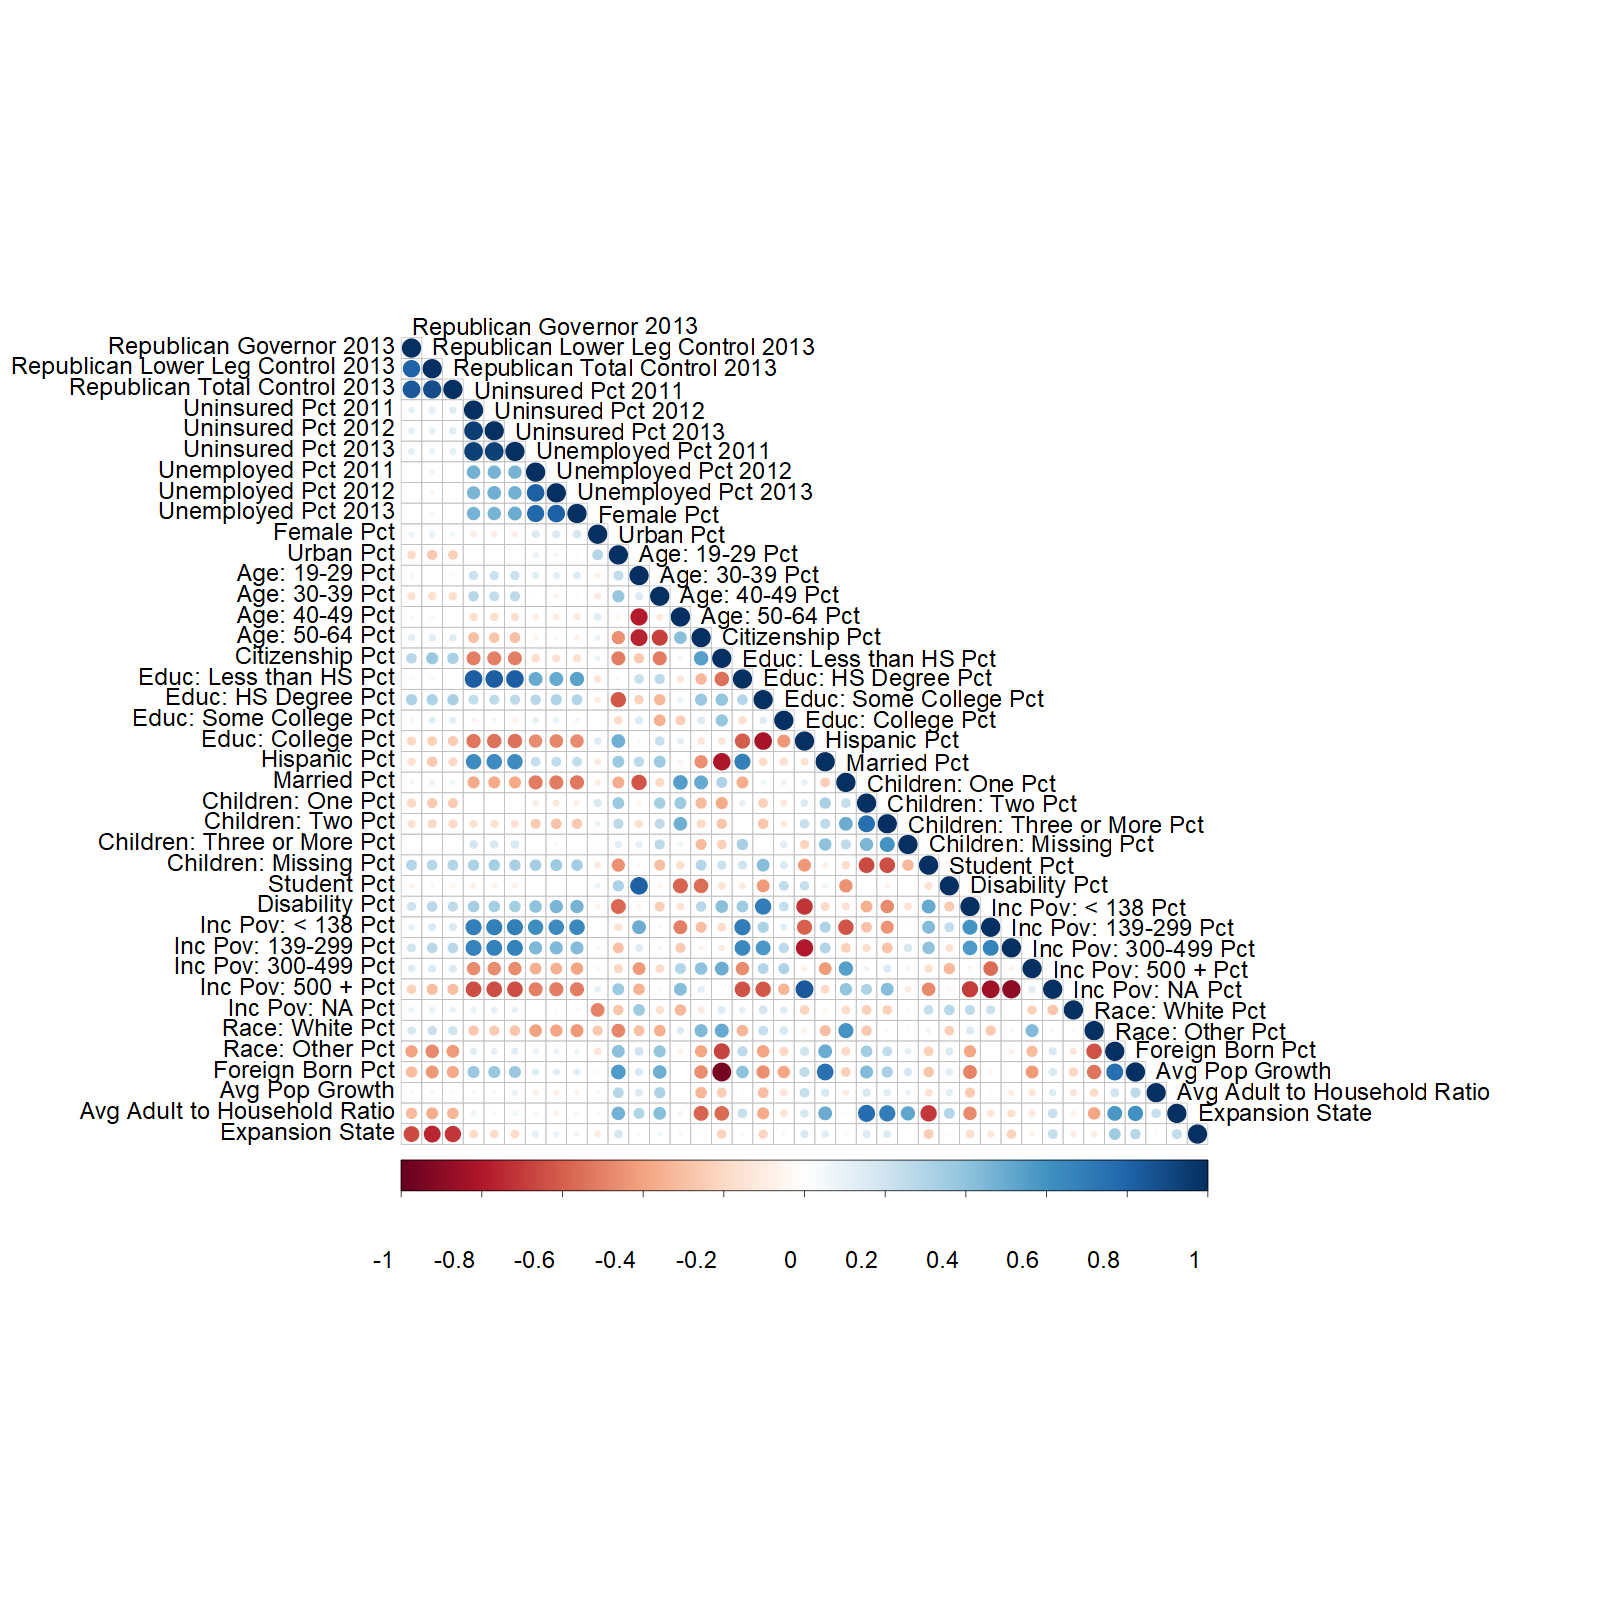
\includegraphics[scale=0.25]{01_Plots/correlation-plot-c1-sigma-zero.png}
\end{center}
\end{figure}

\clearpage

\begin{landscape}

\section{Weight Diagnostics}
\label{ssec:balancetables}

Table~\ref{tab:baltab1} displays the differences between the weighted mean covariate values of the expansion region and the mean of the non-expansion region for our primary dataset and with the early expansion states excluded (calculated using our the homogeneous covariate adjustments). The weights presented here are for the H-SBW estimator. The values under each column are in the following format: (unweighted difference, weighted difference). ``Primary'' and ``Early excluded'' refer to the primary dataset and those that exclude the early expansion states. ``Percent'' indicates that the differences displayed are in percentage points while ``Standardized'' indicates that the standardized mean differences are displayed. Additional results are available on request.

\begin{table}[h!]
\centering
    \caption{Balance table: percent and standardized mean differences, H-SBW weights}
    \label{tab:baltab1}
\begin{tabular}{lllll}
  \hline
Variables & Preferred (Percent) & Preferred (Standardized) & Early excluded (Percent) & Early excluded (Standardized) \\ 
  \hline
Age: 19-29 Pct & (-0.34, -0.34) & (-0.05, -0.05) & (-0.62, -0.21) & (-0.09, -0.03) \\ 
  Age: 30-39 Pct & (0.36, 0.17) & (0.1, 0.05) & (-0.04, 0.32) & (-0.01, 0.09) \\ 
  Age: 40-49 Pct & (0.19, -0.3) & (0.06, -0.1) & (-0.01, -0.44) & (0, -0.15) \\ 
  Avg Adult to Household Ratio & (11.29, -0.04) & (0.37, 0) & (3.37, 0.1) & (0.13, 0) \\ 
  Citizenship Pct & (-3.61, -1.59) & (-0.33, -0.15) & (-0.24, -1.45) & (-0.03, -0.16) \\ 
  Disability Pct & (-1.45, 0.52) & (-0.27, 0.1) & (-0.17, 0.63) & (-0.03, 0.11) \\ 
  Educ: HS Degree Pct & (-3.37, 0.54) & (-0.32, 0.05) & (-1.02, 0.64) & (-0.1, 0.06) \\ 
  Educ: Less than HS Pct & (-0.37, 0.83) & (-0.04, 0.1) & (-1.22, 0.76) & (-0.16, 0.1) \\ 
  Educ: Some College Pct & (-0.35, 0.4) & (-0.05, 0.06) & (0.36, 0.57) & (0.05, 0.08) \\ 
  Female Pct & (-0.34, -0.64) & (-0.16, -0.3) & (-0.25, -1) & (-0.12, -0.48) \\ 
  Foreign Born Pct & (7.6, 2) & (0.42, 0.11) & (1.02, 2) & (0.07, 0.13) \\ 
  Uninsured Pct 2011 & (-3.08, 0.05) & (-0.28, 0) & (-3.51, -0.05) & (-0.34, 0) \\ 
  Uninsured Pct 2012 & (-3, -0.05) & (-0.27, 0) & (-3.4, 0.05) & (-0.33, 0) \\ 
  Uninsured Pct 2013 & (-2.99, -0.05) & (-0.27, 0) & (-3.45, -0.05) & (-0.34, 0) \\ 
  Hispanic Pct & (4.46, 1) & (0.2, 0.04) & (-1.35, 1) & (-0.07, 0.05) \\ 
  Inc Pov: $<$ 138 Pct & (-2.05, 0.63) & (-0.19, 0.06) & (-1.33, 0.12) & (-0.12, 0.01) \\ 
  Inc Pov: 139-299 Pct & (-2.45, 0.65) & (-0.35, 0.09) & (-1.53, 0.5) & (-0.23, 0.08) \\ 
  Inc Pov: 300-499 Pct & (-0.59, -0.18) & (-0.12, -0.04) & (0.28, -0.18) & (0.06, -0.04) \\ 
  Inc Pov: 500 + Pct & (5.58, -1.3) & (0.35, -0.08) & (2.9, -1.23) & (0.2, -0.08) \\ 
  Married Pct & (-0.76, -0.43) & (-0.07, -0.04) & (-0.21, -0.53) & (-0.02, -0.05) \\ 
  Children: Missing Pct & (-3.25, -1) & (-0.36, -0.11) & (-1.99, -0.1) & (-0.21, -0.01) \\ 
  Children: One Pct & (0.7, -0.14) & (0.25, -0.05) & (0.11, -0.31) & (0.04, -0.12) \\ 
  Avg Pop Growth & (-0.09, -0.21) & (-0.07, -0.18) & (-0.26, -0.19) & (-0.22, -0.16) \\ 
  Race: White Pct & (-4.02, 1) & (-0.16, 0.04) & (0.09, 1) & (0, 0.04) \\ 
  Republican Governor 2013 & (-64.78, -25) & (-1.28, -0.5) & (-54.46, -24.87) & (-1.02, -0.47) \\ 
  Republican Lower Leg Control 2013 & (-74.72, -25) & (-1.69, -0.57) & (-56.67, -23.6) & (-1.12, -0.47) \\ 
  Republican Total Control 2013 & (-71.3, -25) & (-1.45, -0.51) & (-56.47, -25) & (-1.02, -0.45) \\ 
  Student Pct & (0.25, -0.5) & (0.04, -0.08) & (0.11, -0.25) & (0.02, -0.04) \\ 
  Children: Three or More Pct & (0, -0.21) & (0, -0.08) & (-0.17, -0.26) & (-0.07, -0.11) \\ 
  Children: Two Pct & (0.76, -0.31) & (0.23, -0.09) & (0.17, -0.37) & (0.05, -0.12) \\ 
  Unemployed Pct 2011 & (0.82, 0.15) & (0.18, 0.03) & (0.68, 0.15) & (0.15, 0.03) \\ 
  Unemployed Pct 2012 & (0.63, -0.03) & (0.14, -0.01) & (0.47, -0.03) & (0.11, -0.01) \\ 
  Unemployed Pct 2013 & (0.42, -0.15) & (0.11, -0.04) & (0.22, -0.15) & (0.06, -0.04) \\ 
  Urban Pct & (8.28, -2) & (0.26, -0.06) & (2.79, -2) & (0.08, -0.06) \\ 
   \hline
\end{tabular}
    \begin{tablenotes}
      \small
      \item The values displayed in each cell are the (weighted, unweighted) differences. The columns containing ``Standardized'' reflect the standardized mean differences while ``percent'' indicates the mean differences in percentage points. The columns containing ``Preferred'' indicate that this is for our primary analysis while ``Early excluded'' is for our analysis that excludes the early expansion states.
    \end{tablenotes}
\end{table}

Figure~\ref{fig:weightsbystatec2} display the weights summed by states when excluding the early expansion states for the H-SBW and BC-HSBW estimators.

\begin{figure}[H]
\begin{center}
    \caption{Total weights summed by state, early expansion removed}
    \label{fig:weightsbystatec2}
    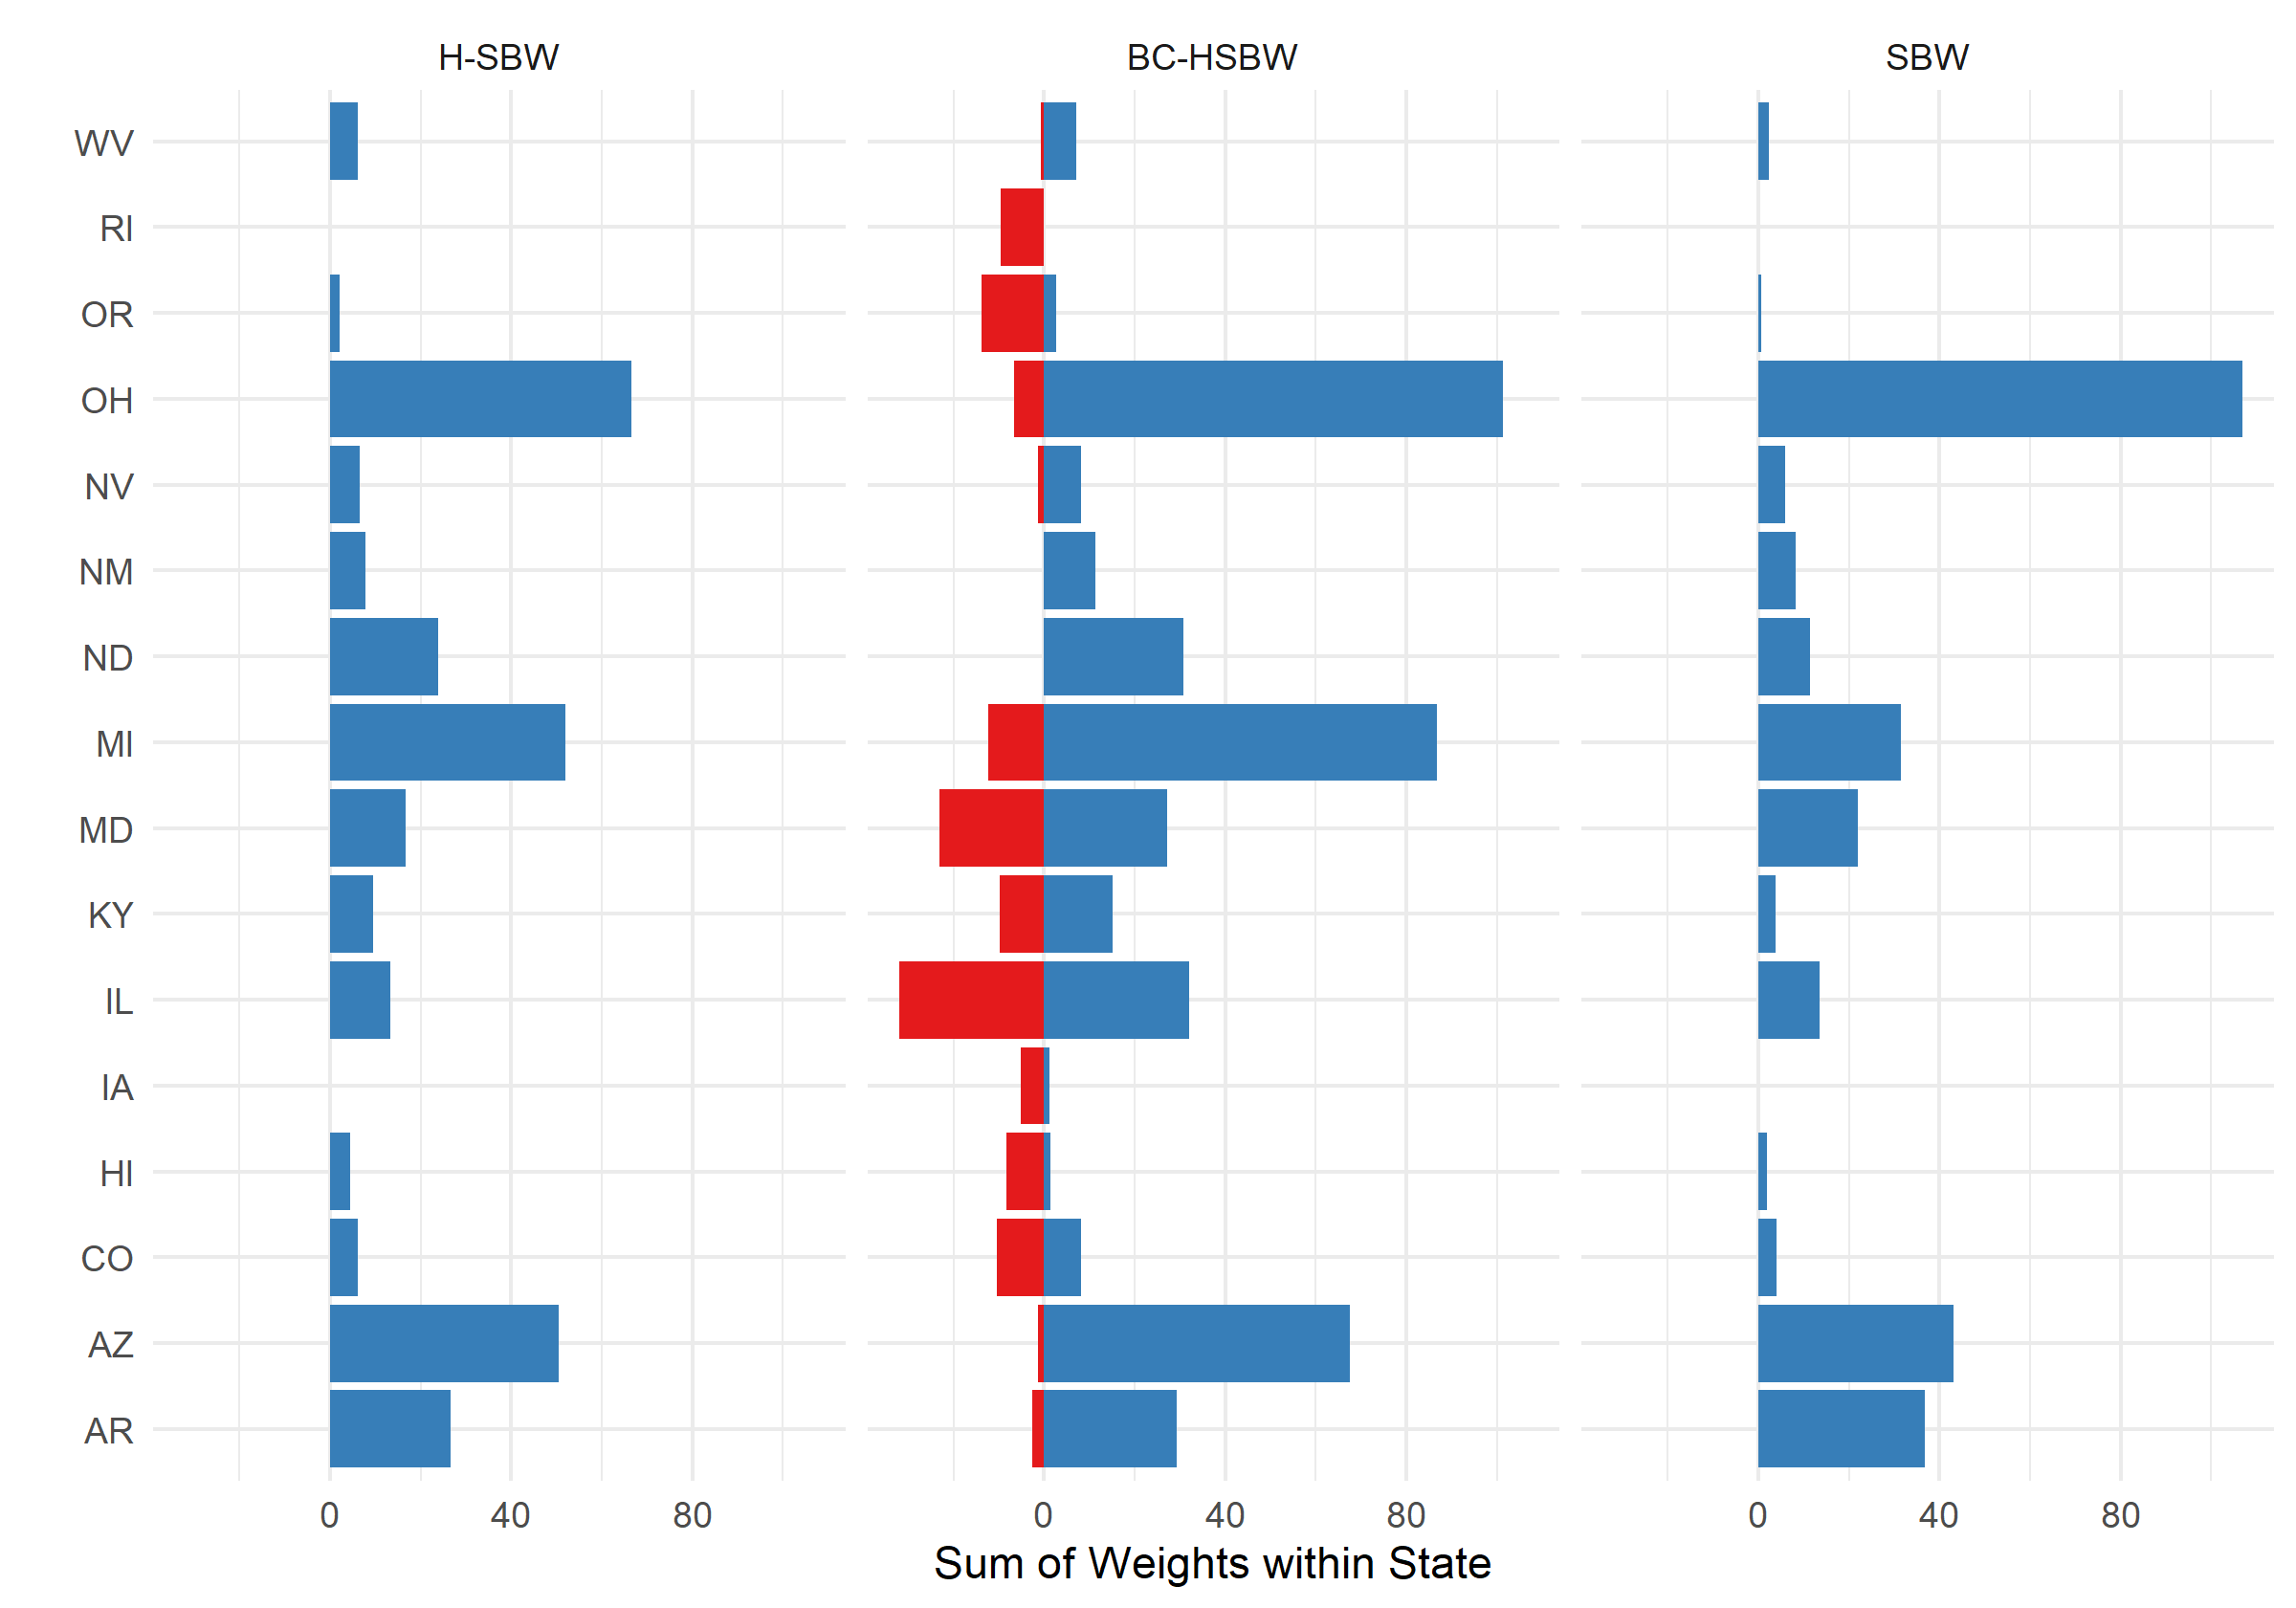
\includegraphics[scale=0.5]{01_Plots/weights-by-state-sbw-hsbw-c2-color.png}
\end{center}
\end{figure}
\end{landscape}
\clearpage

\section{Additional Results}
\label{ssec:allresults}

Table~\ref{tab:confintmain} displays the point estimates from all estimators as well as confidence intervals calculated either (a) leave-one-state-out jackknife on the adjusted dataset (CI (states)); (b) leave-one-state-out jackknife repeating the entire adjusted leaving each state out (CI (proc)). This table also includes all analyses calculated on a second version of the adjusted data where we use a common $\kappa$ for all values (sigma\_uu\_avg), which is the adjustment suggested by \cite{carroll2006measurement}. Notice that the confidence intervals are identical for ``sigma\_zero'' because this is the unadjusted dataset. ``sigma\_uu\_i'' is our preferred covariate adjustment.

\begin{table}[ht]
\centering
\caption{Point estimates and confidence intervals, primary dataset}
\label{tab:confintmain}
\begin{tabular}{llrll}
  \hline
Weight type & Sigma estimate & Psihat & CI (states) & CI (proc) \\ 
  \hline
H-SBW & sigma\_uu\_i & -2.17 & (-3.41, -0.94) & (-3.42, -0.92) \\ 
  H-SBW & sigma\_uu\_avg & -2.25 & (-3.51, -0.99) & (-3.35, -1.14) \\ 
  H-SBW & sigma\_zero & -2.35 & (-3.09, -1.61) & (-3.09, -1.61) \\ 
  BC-HSBW & sigma\_uu\_i & -2.13 & (-3.55, -0.71) & (-3.42, -0.84) \\ 
  BC-HSBW & sigma\_uu\_avg & -2.17 & (-3.57, -0.78) & (-3.39, -0.96) \\ 
  BC-HSBW & sigma\_zero & -2.40 & (-3.33, -1.46) & (-3.33, -1.46) \\ 
  SBW & sigma\_uu\_i & -2.24 & (-3.50, -0.99) & (-3.51, -0.97) \\ 
  SBW & sigma\_uu\_avg & -2.30 & (-3.67, -0.92) & (-3.45, -1.15) \\ 
  SBW & sigma\_zero & -2.40 & (-3.10, -1.69) & (-3.10, -1.69) \\ 
  BC-SBW & sigma\_uu\_i & -2.12 & (-3.15, -1.10) & (-3.11, -1.14) \\ 
  BC-SBW & sigma\_uu\_avg & -2.17 & (-3.25, -1.08) & (-3.22, -1.12) \\ 
  BC-SBW & sigma\_zero & -2.36 & (-2.93, -1.80) & (-2.93, -1.80) \\ 
   \hline
\end{tabular}
\end{table}

Table~\ref{tab:ptests} presents all point estimates from estimators that we calculated. The ``Var subset`` column indicates which variables were excluded from the estimation: 0 excludes no variables; 1 removes Republican governance indicators; 2 pre-treatment uninsurance and unemployment rates; 3 urban, age, education, citizenship, marital status, student, disability, or female; 4 race, ethnicity, income, foreign born; 5 children, population growth, and household to person ratio. We see that the largest changes generally occur when excluding the pre-treatment uninsurance and unemployment rates. This is not surprising: controlling for the other covariates, the pre-treatment uninsurance rate was substantially lower in the treated region compared to the control region. Given that pre-treatment uninsurance rates are highly correlated with post-treatment rates, we find that this comparison leads to a larger absolute magnitude point estimate, highlighting the need to control for these covariates.

%Wed Jan 13 15:24:43 2021
\begin{table}[ht]
\centering
\caption{Point estimates for all specifications}
\label{tab:ptests}
\begin{tabular}{rlrrrr}
  \hline
Variable subset & Sigma estimate & H-SBW & BC-HSBW & SBW & BC-SBW \\ 
  \hline
0 & sigma\_uu\_i & -2.17 & -2.13 & -2.24 & -2.12 \\ 
  0 & sigma\_uu\_avg & -2.25 & -2.17 & -2.30 & -2.17 \\ 
  0 & sigma\_zero & -2.35 & -2.40 & -2.40 & -2.36 \\ 
  1 & sigma\_uu\_i & -2.85 & -2.87 & -3.00 & -2.76 \\ 
  1 & sigma\_uu\_avg & -2.86 & -2.86 & -2.99 & -2.75 \\ 
  1 & sigma\_zero & -3.00 & -3.09 & -3.07 & -2.92 \\ 
  2 & sigma\_uu\_i & -5.73 & -5.05 & -5.24 & -4.70 \\ 
  2 & sigma\_uu\_avg & -5.73 & -5.05 & -5.24 & -4.70 \\ 
  2 & sigma\_zero & -5.73 & -5.13 & -5.24 & -4.77 \\ 
  3 & sigma\_uu\_i & -2.17 & -2.00 & -2.24 & -2.00 \\ 
  3 & sigma\_uu\_avg & -2.25 & -2.06 & -2.29 & -2.06 \\ 
  3 & sigma\_zero & -2.34 & -2.17 & -2.40 & -2.15 \\ 
  4 & sigma\_uu\_i & -2.35 & -2.39 & -2.29 & -2.30 \\ 
  4 & sigma\_uu\_avg & -2.39 & -2.39 & -2.32 & -2.32 \\ 
  4 & sigma\_zero & -2.45 & -2.59 & -2.43 & -2.49 \\ 
  5 & sigma\_uu\_i & -2.17 & -2.19 & -2.26 & -2.21 \\ 
  5 & sigma\_uu\_avg & -2.25 & -2.24 & -2.33 & -2.27 \\ 
  5 & sigma\_zero & -2.35 & -2.44 & -2.42 & -2.47 \\ 
   \hline
\end{tabular}
\end{table}

Table ~\ref{tab:confintmainc2} and Table~\ref{tab:secondaryptests} are identical to the structure of the previous two tables except we exclude the ``early expansion states'' from the pool of expansion state matches. 

\begin{table}[ht]
\centering
\caption{Point estimates and confidence intervals, early expansion excluded}
\label{tab:confintmainc2}
\begin{tabular}{llrll}
  \hline
Weight type & Sigma estimate & Psihat & CI (states) & CI (proc) \\ 
  \hline
H-SBW & sigma\_uu\_i & -2.05 & (-3.10, -1.00) & (-3.05, -1.05) \\ 
  H-SBW & sigma\_uu\_avg & -2.13 & (-3.20, -1.05) & (-3.17, -1.08) \\ 
  H-SBW & sigma\_zero & -2.29 & (-2.90, -1.69) & (-2.90, -1.69) \\ 
  BC-HSBW & sigma\_uu\_i & -2.14 & (-3.63, -0.64) & (-3.48, -0.80) \\ 
  BC-HSBW & sigma\_uu\_avg & -2.19 & (-3.65, -0.73) & (-3.57, -0.81) \\ 
  BC-HSBW & sigma\_zero & -2.50 & (-3.66, -1.33) & (-3.66, -1.33) \\ 
  SBW & sigma\_uu\_i & -1.91 & (-2.91, -0.91) & (-2.79, -1.03) \\ 
  SBW & sigma\_uu\_avg & -2.01 & (-3.02, -1.00) & (-2.83, -1.19) \\ 
  SBW & sigma\_zero & -2.20 & (-2.69, -1.71) & (-2.69, -1.71) \\ 
  BC-SBW & sigma\_uu\_i & -1.97 & (-3.49, -0.44) & (-3.27, -0.66) \\ 
  BC-SBW & sigma\_uu\_avg & -2.04 & (-3.59, -0.50) & (-3.39, -0.70) \\ 
  BC-SBW & sigma\_zero & -2.34 & (-3.44, -1.25) & (-3.44, -1.25) \\ 
   \hline
\end{tabular}
\end{table}

\begin{table}[ht]
\centering
   \caption{Point estimates for all specifications, early expansion excluded}
    \label{tab:secondaryptests}
\begin{tabular}{rlrrrr}
  \hline
Variable subset & Sigma estimate & H-SBW & BC-HSBW & SBW & BC-SBW \\ 
  \hline
0 & sigma\_uu\_i & -2.05 & -2.14 & -1.91 & -1.97 \\ 
  0 & sigma\_uu\_avg & -2.13 & -2.19 & -2.01 & -2.04 \\ 
  0 & sigma\_zero & -2.29 & -2.50 & -2.20 & -2.34 \\ 
  1 & sigma\_uu\_i & -2.85 & -2.99 & -2.85 & -2.86 \\ 
  1 & sigma\_uu\_avg & -2.86 & -2.98 & -2.86 & -2.86 \\ 
  1 & sigma\_zero & -3.05 & -3.18 & -2.96 & -2.99 \\ 
  2 & sigma\_uu\_i & -5.55 & -4.46 & -5.02 & -4.52 \\ 
  2 & sigma\_uu\_avg & -5.55 & -4.73 & -5.01 & -4.53 \\ 
  2 & sigma\_zero & -5.55 & -4.78 & -5.01 & -4.56 \\ 
  3 & sigma\_uu\_i & -2.05 & -2.03 & -1.91 & -1.89 \\ 
  3 & sigma\_uu\_avg & -2.13 & -2.10 & -2.00 & -1.97 \\ 
  3 & sigma\_zero & -2.27 & -2.22 & -2.20 & -2.13 \\ 
  4 & sigma\_uu\_i & -2.27 & -2.24 & -2.15 & -2.00 \\ 
  4 & sigma\_uu\_avg & -2.35 & -2.28 & -2.23 & -2.04 \\ 
  4 & sigma\_zero & -2.36 & -2.62 & -2.28 & -2.45 \\ 
  5 & sigma\_uu\_i & -2.05 & -2.20 & -1.91 & -2.03 \\ 
  5 & sigma\_uu\_avg & -2.13 & -2.26 & -1.99 & -2.11 \\ 
  5 & sigma\_zero & -2.29 & -2.45 & -2.19 & -2.36 \\ 
   \hline
\end{tabular}
\end{table}

Table~\ref{tab:loostatec1} and Table~\ref{tab:loostatec2} present point estimates for the leave-one-state out analysis for our preferred estimator, H-SBW calculated on our preferred covariate adjustment for the primary dataset and when excluding early expansion states.

\begin{table}[ht]
\centering
   \caption{Leave-one-state-out point estimates, primary dataset, preferred adjustment}
    \label{tab:loostatec1}
\begin{tabular}{lrlrl}
  \hline
State & Psihat (0) & None (states, proc) & Psihat (1) & Repub (states, proc) \\ 
  \hline
AR & -2.17 & (-2.34, -2.38) & -2.85 & (-2.81, -2.80) \\ 
  AZ & -2.17 & (-2.21, -2.24) & -2.85 & (-2.86, -2.86) \\ 
  CA & -2.17 & (-1.99, -2.02) & -2.85 & (-2.77, -2.76) \\ 
  CO & -2.17 & (-2.17, -2.23) & -2.85 & (-2.84, -2.84) \\ 
  CT & -2.17 & (-2.17, -2.15) & -2.85 & (-2.83, -2.82) \\ 
  HI & -2.17 & (-2.15, -2.14) & -2.85 & (-2.77, -2.78) \\ 
  IA & -2.17 & (-2.09, -2.07) & -2.85 & (-2.83, -2.84) \\ 
  IL & -2.17 & (-2.16, -2.24) & -2.85 & (-2.83, -2.84) \\ 
  KY & -2.17 & (-2.02, -1.95) & -2.85 & (-2.57, -2.52) \\ 
  MD & -2.17 & (-2.25, -2.27) & -2.85 & (-2.94, -2.94) \\ 
  MI & -2.17 & (-2.10, -2.18) & -2.85 & (-2.89, -2.92) \\ 
  MN & -2.17 & (-2.17, -2.19) & -2.85 & (-2.84, -2.86) \\ 
  ND & -2.17 & (-2.23, -2.26) & -2.85 & (-2.84, -2.84) \\ 
  NH & -2.17 & (-2.18, -2.21) & -2.85 & (-2.98, -2.99) \\ 
  NJ & -2.17 & (-2.26, -2.25) & -2.85 & (-2.99, -3.03) \\ 
  NM & -2.17 & (-2.16, -2.22) & -2.85 & (-2.76, -2.77) \\ 
  NV & -2.17 & (-2.21, -2.24) & -2.85 & (-2.89, -2.88) \\ 
  OH & -2.17 & (-2.70, -2.68) & -2.85 & (-3.00, -2.98) \\ 
  OR & -2.17 & (-2.17, -2.25) & -2.85 & (-2.80, -2.84) \\ 
  RI & -2.17 & (-2.17, -2.15) & -2.85 & (-2.81, -2.81) \\ 
  WA & -2.17 & (-2.10, -2.11) & -2.85 & (-2.78, -2.77) \\ 
  WV & -2.17 & (-2.16, -2.18) & -2.85 & (-2.8, -2.78) \\ 
   \hline
\end{tabular}
\end{table}

\begin{table}[ht]
\centering
   \caption{Leave-one-state-out point estimates, early expansion excluded, preferred adjustment}
    \label{tab:loostatec2}
\begin{tabular}{lrlrl}
  \hline
State & Psihat (0) & None (states, proc) & Psihat (1) & Repub (states, proc) \\ 
  \hline
AR & -2.05 & (-2.15, -2.16) & -2.85 & (-2.77, -2.76) \\ 
  AZ & -2.05 & (-1.82, -1.88) & -2.85 & (-2.87, -2.86) \\ 
  CO & -2.05 & (-2.07, -2.09) & -2.85 & (-2.84, -2.83) \\ 
  HI & -2.05 & (-2.01, -1.99) & -2.85 & (-2.71, -2.73) \\ 
  IA & -2.05 & (-1.98, -1.95) & -2.85 & (-2.85, -2.86) \\ 
  IL & -2.05 & (-2.03, -2.01) & -2.85 & (-2.8, -2.79) \\ 
  KY & -2.05 & (-1.87, -1.8) & -2.85 & (-2.59, -2.54) \\ 
  MD & -2.05 & (-2.18, -2.15) & -2.85 & (-2.97, -2.96) \\ 
  MI & -2.05 & (-1.96, -2) & -2.85 & (-2.92, -2.96) \\ 
  ND & -2.05 & (-2.02, -2.04) & -2.85 & (-2.84, -2.84) \\ 
  NH & -2.05 & (-2.05, -2.06) & -2.85 & (-3.02, -3.03) \\ 
  NM & -2.05 & (-1.99, -1.97) & -2.85 & (-2.72, -2.75) \\ 
  NV & -2.05 & (-2.15, -2.15) & -2.85 & (-2.93, -2.92) \\ 
  OH & -2.05 & (-2.43, -2.38) & -2.85 & (-3.03, -3.02) \\ 
  OR & -2.05 & (-2.05, -2.11) & -2.85 & (-2.81, -2.84) \\ 
  RI & -2.05 & (-2.05, -2.05) & -2.85 & (-2.80, -2.80) \\ 
  WV & -2.05 & (-2.06, -2.06) & -2.85 & (-2.83, -2.81) \\ 
   \hline
\end{tabular}
\end{table}

Table~\ref{tab:oateconfint} displays point estimates and confidence intervals for the primary point estimates for the OATE. We display the confidence intervals calculated using both the leave-one-out-states conditional on the covariate adjustment (CI (states)) and recalculating the covariate adjustment for the OATE (CI (proc)). 

\begin{table}[ht]
\centering
\caption{OATE primary results inference}
\label{tab:oateconfint}
\begin{tabular}{rllll}
  \hline
Psihat & Sigma estimate & Dataset & CI (states) & CI (proc) \\ 
  \hline
-1.74 & sigma\_uu\_i\_modeled & c1 & (-2.35, -1.14) & (-2.48, -1.00) \\ 
  -1.67 & sigma\_uu\_avg & c1 & (-2.34, -0.99) & (-2.52, -0.81) \\ 
  -1.80 & sigma\_zero & c1 & (-2.50, -1.10) & (-2.50, -1.10) \\ 
  -1.89 & sigma\_uu\_i\_modeled & c2 & (-2.47, -1.32) & (-2.54, -1.24) \\ 
  -1.80 & sigma\_uu\_avg & c2 & (-2.43, -1.17) & (-2.57, -1.03) \\ 
  -1.95 & sigma\_zero & c2 & (-2.65, -1.25) & (-2.65, -1.25) \\ 
   \hline
\end{tabular}
\end{table}

Table~\ref{tab:oatesensitive} presents all point estimates calculate using the overlap weights. Dataset ``c1'' refers to the primary dataset and dataset ``c2'' removes the early expansion states. The numeric column names refer to the covariate group excluded (covariate groups described above).

\begin{table}[ht]
\centering
\caption{OATE all point estimates}
\label{tab:oatesensitive}
\begin{tabular}{llrrrrrr}
  \hline
Sigma estimate & Dataset & 0 & 1 & 2 & 3 & 4 & 5 \\ 
  \hline
sigma\_uu\_i & c1 & -1.64 & -2.60 & -2.96 & -1.86 & -1.86 & -1.77 \\ 
  sigma\_uu\_i & c2 & -1.81 & -2.53 & -3.10 & -2.18 & -2.04 & -1.96 \\ 
  sigma\_avg & c1 & -1.58 & -2.62 & -2.85 & -1.76 & -1.76 & -1.78 \\ 
  sigma\_avg & c2 & -1.74 & -2.54 & -3.00 & -2.10 & -1.96 & -1.95 \\ 
  sigma\_zero & c1 & -1.80 & -2.55 & -3.11 & -1.98 & -1.94 & -1.83 \\ 
  sigma\_zero & c2 & -1.95 & -2.51 & -3.25 & -2.12 & -2.10 & -2.00 \\ 
   \hline
\end{tabular}
\end{table}

Table~\ref{tab:rdiffc1} and ~\ref{tab:rdiffc2} display the quantiles of the distribution $\hat{\Delta}_v^1$ estimates when leaving out each state for the primary dataset and removing the early expansion states. The ``resample'' column indicates whether the entire adjustment procedure was recalculated (``proc'') or whether we left out each state conditional on the adjustment (``states''). Table~\ref{tab:hte} displays the estimated linear combination of model coefficients on the Republican governance indicators with 95 percent confidence intervals (standard errors clustered at the state level). The ``Weights'' column represents whether the regressions were weighted; we ran two versions, an unweighted regression and one using the overlap weights.

\begin{table}[ht]
\centering
\label{tab:rdiffc1}
\caption{$\hat{\Delta}^1_v$ leave-one-state-out estimates, primary dataset}
\begin{tabular}{lllrrrrrr}
  \hline
Resample & Sigma estimate & Weight type & Original & 0\% & 25\% & 50\% & 75\% & 100\% \\ 
  \hline
states & sigma\_uu\_i\_modeled & H-SBW & -0.67 & -0.80 & -0.68 & -0.67 & -0.62 & -0.30 \\ 
  proc & sigma\_uu\_i\_modeled & H-SBW & -0.67 & -0.78 & -0.68 & -0.64 & -0.59 & -0.30 \\ 
  states & sigma\_uu\_i\_modeled & BC-HSBW & -0.74 & -0.87 & -0.77 & -0.71 & -0.69 & -0.26 \\ 
  proc & sigma\_uu\_i\_modeled & BC-HSBW & -0.74 & -0.85 & -0.76 & -0.70 & -0.67 & -0.34 \\ 
  states & sigma\_uu\_i\_modeled & SBW & -0.75 & -0.98 & -0.77 & -0.75 & -0.72 & -0.48 \\ 
  proc & sigma\_uu\_i\_modeled & SBW & -0.75 & -0.98 & -0.78 & -0.73 & -0.67 & -0.49 \\ 
  states & sigma\_uu\_i\_modeled & BC-SBW & -0.63 & -0.85 & -0.69 & -0.62 & -0.61 & -0.39 \\ 
  proc & sigma\_uu\_i\_modeled & BC-SBW & -0.63 & -0.82 & -0.68 & -0.64 & -0.59 & -0.35 \\ 
  states & sigma\_uu\_avg & H-SBW & -0.61 & -0.74 & -0.64 & -0.60 & -0.57 & -0.23 \\ 
  proc & sigma\_uu\_avg & H-SBW & -0.61 & -0.76 & -0.63 & -0.59 & -0.55 & -0.33 \\ 
  states & sigma\_uu\_avg & BC-HSBW & -0.69 & -0.83 & -0.73 & -0.68 & -0.64 & -0.24 \\ 
  proc & sigma\_uu\_avg & BC-HSBW & -0.69 & -0.83 & -0.73 & -0.66 & -0.63 & -0.39 \\ 
  states & sigma\_uu\_avg & SBW & -0.70 & -0.89 & -0.72 & -0.69 & -0.67 & -0.31 \\ 
  proc & sigma\_uu\_avg & SBW & -0.70 & -0.93 & -0.73 & -0.68 & -0.65 & -0.49 \\ 
  states & sigma\_uu\_avg & BC-SBW & -0.58 & -0.78 & -0.63 & -0.57 & -0.56 & -0.32 \\ 
  proc & sigma\_uu\_avg & BC-SBW & -0.58 & -0.81 & -0.63 & -0.58 & -0.55 & -0.28 \\ 
  states & sigma\_zero & H-SBW & -0.65 & -0.78 & -0.66 & -0.63 & -0.61 & -0.50 \\ 
  proc & sigma\_zero & H-SBW & -0.65 & -0.78 & -0.66 & -0.63 & -0.61 & -0.50 \\ 
  states & sigma\_zero & BC-HSBW & -0.70 & -0.88 & -0.74 & -0.68 & -0.64 & -0.50 \\ 
  proc & sigma\_zero & BC-HSBW & -0.70 & -0.88 & -0.74 & -0.68 & -0.64 & -0.50 \\ 
  states & sigma\_zero & SBW & -0.68 & -0.84 & -0.71 & -0.68 & -0.66 & -0.49 \\ 
  proc & sigma\_zero & SBW & -0.68 & -0.84 & -0.71 & -0.68 & -0.66 & -0.49 \\ 
  states & sigma\_zero & BC-SBW & -0.56 & -0.67 & -0.61 & -0.55 & -0.52 & -0.39 \\ 
  proc & sigma\_zero & BC-SBW & -0.56 & -0.67 & -0.61 & -0.55 & -0.52 & -0.39 \\ 
   \hline
\end{tabular}
\end{table}

\begin{table}[ht]
\label{tab:rdiffc2}
\caption{$\hat{\Delta}^1_v$ leave-one-state-out estimates, early expansion excluded}
\centering
\begin{tabular}{lllrrrrrr}
  \hline
Resample & Sigma estimate & Weight type & Original & 0\% & 25\% & 50\% & 75\% & 100\% \\ 
  \hline
states & sigma\_uu\_i\_modeled & H-SBW & -0.80 & -1.05 & -0.82 & -0.77 & -0.73 & -0.60 \\ 
  proc & sigma\_uu\_i\_modeled & H-SBW & -0.80 & -0.98 & -0.81 & -0.76 & -0.74 & -0.60 \\ 
  states & sigma\_uu\_i\_modeled & BC-HSBW & -0.85 & -1.13 & -0.96 & -0.83 & -0.76 & -0.45 \\ 
  proc & sigma\_uu\_i\_modeled & BC-HSBW & -0.85 & -1.05 & -0.94 & -0.83 & -0.77 & -0.53 \\ 
  states & sigma\_uu\_i\_modeled & SBW & -0.94 & -1.15 & -0.94 & -0.92 & -0.89 & -0.70 \\ 
  proc & sigma\_uu\_i\_modeled & SBW & -0.94 & -1.05 & -0.98 & -0.91 & -0.86 & -0.73 \\ 
  states & sigma\_uu\_i\_modeled & BC-SBW & -0.89 & -1.27 & -0.93 & -0.86 & -0.81 & -0.26 \\ 
  proc & sigma\_uu\_i\_modeled & BC-SBW & -0.89 & -1.19 & -0.96 & -0.86 & -0.81 & -0.37 \\ 
  states & sigma\_uu\_avg & H-SBW & -0.73 & -0.99 & -0.74 & -0.70 & -0.68 & -0.51 \\ 
  proc & sigma\_uu\_avg & H-SBW & -0.73 & -0.94 & -0.73 & -0.69 & -0.67 & -0.50 \\ 
  states & sigma\_uu\_avg & BC-HSBW & -0.79 & -1.10 & -0.87 & -0.78 & -0.69 & -0.42 \\ 
  proc & sigma\_uu\_avg & BC-HSBW & -0.79 & -1.01 & -0.89 & -0.73 & -0.69 & -0.46 \\ 
  states & sigma\_uu\_avg & SBW & -0.85 & -1.08 & -0.85 & -0.83 & -0.81 & -0.66 \\ 
  proc & sigma\_uu\_avg & SBW & -0.85 & -0.95 & -0.86 & -0.82 & -0.80 & -0.68 \\ 
  states & sigma\_uu\_avg & BC-SBW & -0.82 & -1.21 & -0.86 & -0.80 & -0.74 & -0.18 \\ 
  proc & sigma\_uu\_avg & BC-SBW & -0.82 & -1.09 & -0.86 & -0.76 & -0.74 & -0.26 \\ 
  states & sigma\_zero & H-SBW & -0.76 & -0.95 & -0.83 & -0.74 & -0.70 & -0.58 \\ 
  proc & sigma\_zero & H-SBW & -0.76 & -0.95 & -0.83 & -0.74 & -0.70 & -0.58 \\ 
  states & sigma\_zero & BC-HSBW & -0.69 & -1.00 & -0.83 & -0.70 & -0.60 & -0.39 \\ 
  proc & sigma\_zero & BC-HSBW & -0.69 & -1.00 & -0.83 & -0.70 & -0.60 & -0.39 \\ 
  states & sigma\_zero & SBW & -0.76 & -0.91 & -0.83 & -0.75 & -0.74 & -0.51 \\ 
  proc & sigma\_zero & SBW & -0.76 & -0.91 & -0.83 & -0.75 & -0.74 & -0.51 \\ 
  states & sigma\_zero & BC-SBW & -0.64 & -1.06 & -0.70 & -0.58 & -0.55 & -0.38 \\ 
  proc & sigma\_zero & BC-SBW & -0.64 & -1.06 & -0.70 & -0.58 & -0.55 & -0.38 \\ 
   \hline
\end{tabular}
\end{table}

\begin{table}[ht]
\caption{OLS HTE estimates}
\label{tab:hte}
\centering
\begin{tabular}{rllll}
  \hline
Estimate & Dataset & Sigma estimate & CI 95 & Weights \\ 
  \hline
  -1.76 & c1 & sigma\_uu\_i\_modeled & (-5.47, 1.94) & Overlap \\ 
  -1.67 & c1 & sigma\_uu\_avg & (-7.18, 3.84) & Overlap \\ 
  -1.97 & c1 & sigma\_zero & (-4.11, 0.17) & Overlap \\ 
  0.51 & c2 & sigma\_uu\_i\_modeled & (-6.00, 7.02) & Overlap \\ 
  -0.17 & c2 & sigma\_uu\_avg & (-8.17, 7.83) & Overlap \\ 
  -1.48 & c2 & sigma\_zero & (-3.51, 0.54) & Overlap \\ 
  0.10 & c1 & sigma\_uu\_i\_modeled & (-1.09, 1.30) & None \\ 
  0.61 & c1 & sigma\_uu\_avg & (-1.82, 3.04) & None \\ 
  -0.12 & c1 & sigma\_zero & (-0.90, 0.66) & None \\ 
  0.37 & c2 & sigma\_uu\_i\_modeled & (-0.9, 1.63) & None \\ 
  0.64 & c2 & sigma\_uu\_avg & (-1.77, 3.04) & None \\ 
  -0.11 & c2 & sigma\_zero & (-0.91, 0.68) & None \\ 
   \hline
\end{tabular}
\end{table}


\end{appendix}

%%%%%%%%%%%%%%%%%%%%%%%%%%%%%%%%%%%%%%%%%%%%%%
%% Support information (funding), if any,   %%
%% should be provided in the                %%
%% Acknowledgements section.                %%
%%%%%%%%%%%%%%%%%%%%%%%%%%%%%%%%%%%%%%%%%%%%%%
\section*{Acknowledgements}

The authors gratefully acknowledge invaluable advice and comments from Zachary Branson, Dave Choi, Edward Kennedy, Brian Kovak, Akshaya Jha, Lowell Taylor, and Jose Zubizaretta.

%%%%%%%%%%%%%%%%%%%%%%%%%%%%%%%%%%%%%%%%%%%%%%
%% Supplementary Material, if any, should   %%
%% be provided in {supplement} environment  %%
%% with title and short description.        %%
%%%%%%%%%%%%%%%%%%%%%%%%%%%%%%%%%%%%%%%%%%%%%%
\begin{supplement}
Analysis programs and supporting materials are available online at github.com/mrubinst757
\end{supplement}

%%%%%%%%%%%%%%%%%%%%%%%%%%%%%%%%%%%%%%%%%%%%%%%%%%%%%%%%%%%%%
%%                  The Bibliography                       %%
%%                                                         %%
%%  imsart-nameyear.bst  will be used to                   %%
%%  create a .BBL file for submission.                     %%
%%                                                         %%
%%  Note that the displayed Bibliography will not          %%
%%  necessarily be rendered by Latex exactly as specified  %%
%%  in the online Instructions for Authors.                %%
%%                                                         %%
%%  MR numbers will be added by VTeX.                      %%
%%                                                         %%
%%  Use \cite{...} to cite references in text.             %%
%%                                                         %%
%%%%%%%%%%%%%%%%%%%%%%%%%%%%%%%%%%%%%%%%%%%%%%%%%%%%%%%%%%%%%

%% if your bibliography is in bibtex format, uncomment commands:
\bibliographystyle{imsart-nameyear} % Style BST file
\bibliography{research.bib}       % Bibliography file (usually '*.bib')

%% or include bibliography directly:
% \begin{thebibliography}{}
% \bibitem[\protect\citeauthoryear{???}{???}]{b1}
% \end{thebibliography}

\end{document}
